\documentclass[12pt]{book}
\usepackage{amsmath}
\usepackage{amsthm}
\usepackage{amssymb}
\usepackage{fontspec}
\usepackage{ctex}
\usepackage{graphicx}
\usepackage{xcolor}
\usepackage{stmaryrd}%输入特定数学符号的宏包,如整数区间符号
\usepackage{wrapfig}%图文混排
\usepackage{caption}%浮动体的标题
\usepackage{subfig}%排列多张图片
\usepackage{float}%[H]参数防止图片浮动到下一页
\usepackage{listings}
\usepackage{framed}
\usepackage{hyperref}
\theoremstyle{definition}\newtheorem{dfn}{Définition}[chapter]
\theoremstyle{plain}\newtheorem{thm}{Théorème}[chapter]
\theoremstyle{plain}\newtheorem{prp}{Proposition}[chapter]
\theoremstyle{plain}\newtheorem{lem}{\bf Lemme}[chapter]
\theoremstyle{plain}\newtheorem{axm}{\bf Axiome}[chapter]
\theoremstyle{plain}\newtheorem{lmm}{\bf Lemme}[chapter]
\theoremstyle{plain}\newtheorem{cor}{\bf Corollaire}[chapter]
\theoremstyle{remark}\newtheorem{rem}{Remarque}[chapter]
\title{Notes of physiques}
\author{PhilippeMENG}
\date{\today}
\lstset{language=Matlab}
\lstset{breaklines}
\lstset{extendedchars=false}
\begin{document}
\maketitle
\tableofcontents
	\chapter{Electrocinétique: cadre et concepts de base}
	\section{Notions sur les phénomènes de conduction}
	\subsection{Sens conventionnel du courant électrique}
	Le courant électrique résulte du déplacement de particules chargées {\color{red} porteurs de charge}. 
	
	因为19世纪人们所知道的各种效应无法确定金属导体介质中的le type des porteurs,所以我们忽略了porteurs所带的电荷符号,并作出如下规定:
	
	
	Le sens conventionnel du courant est celui des porteurs de charges positives.

        
	\subsection{Courant électrique}
	\subsection{Courant dans un circuit}
	\paragraph{Ordre de grandeur de la vitesse des porteurs de charge}
	Pour un fil de cuivre de section $S=1mm^2$,traverse par un courant constant $I=1A$

\subsection{有源二端元件}
\paragraph{理想电源}理想:内阻为极限情况:$0$(理想电压源,内阻与其串联,等效为无分压内阻)或$\infty$(理想电流源,内阻与其并联,等效为无分流内阻).
\\外电路:元件二端(节点或线头)之外的电路\\
理想电压源:输出恒定电压,电流要根据外电路判断
\\理想电流源:输出恒定电流,两端电压要根据外电路判断
\paragraph{实际电源}实际的情况下电路电源由两种模型表述:(注意只是形式上代替了对理想电源的认识)

Thevenin等效模型
\begin{figure}[H]
	\centering
	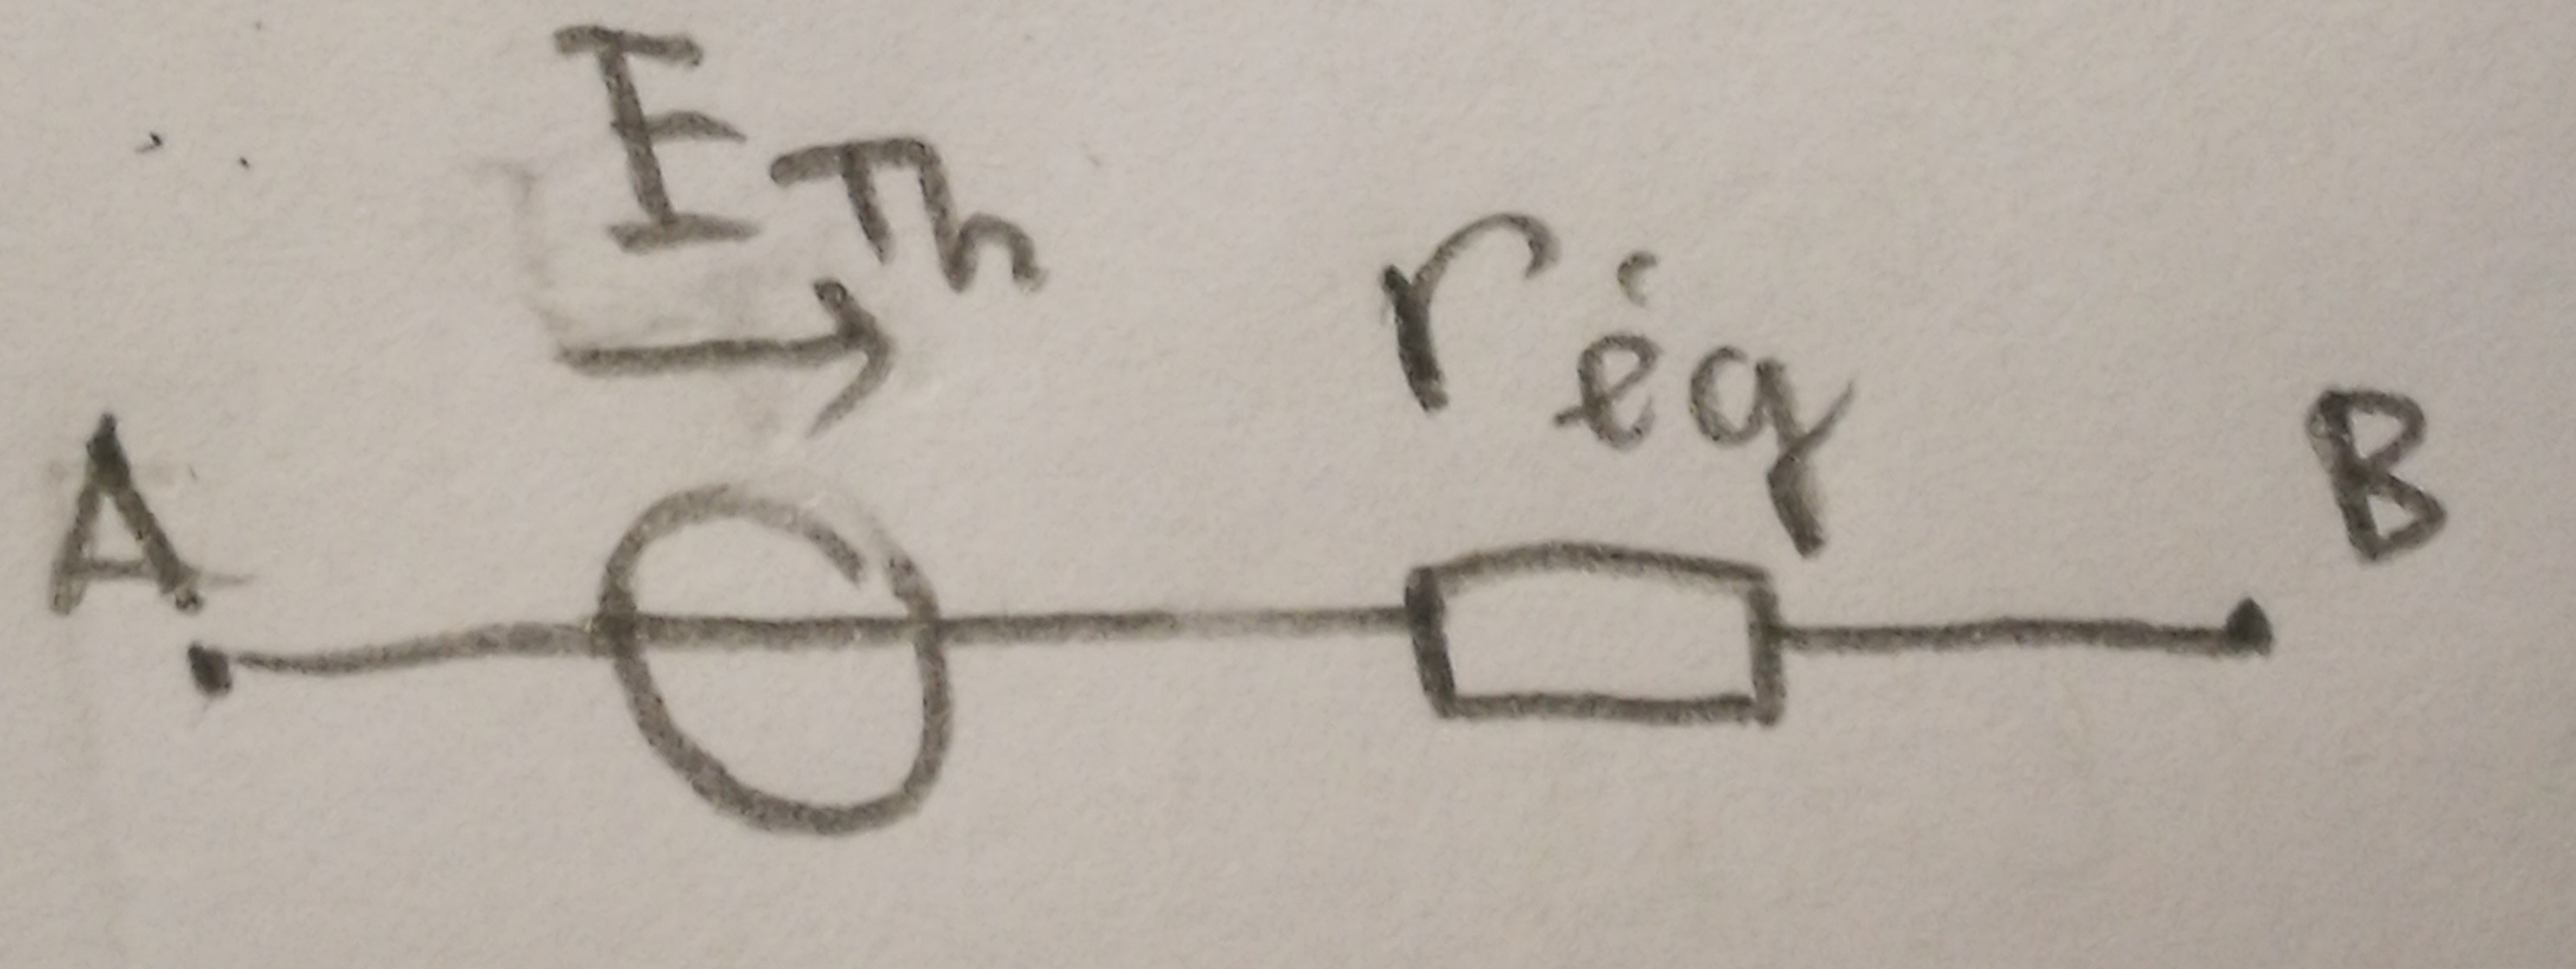
\includegraphics[scale=0.1]{Electrocinetique cadre et concepts de base//1}
\end{figure}
Norton等效模型
\begin{figure}[H]
	\centering
	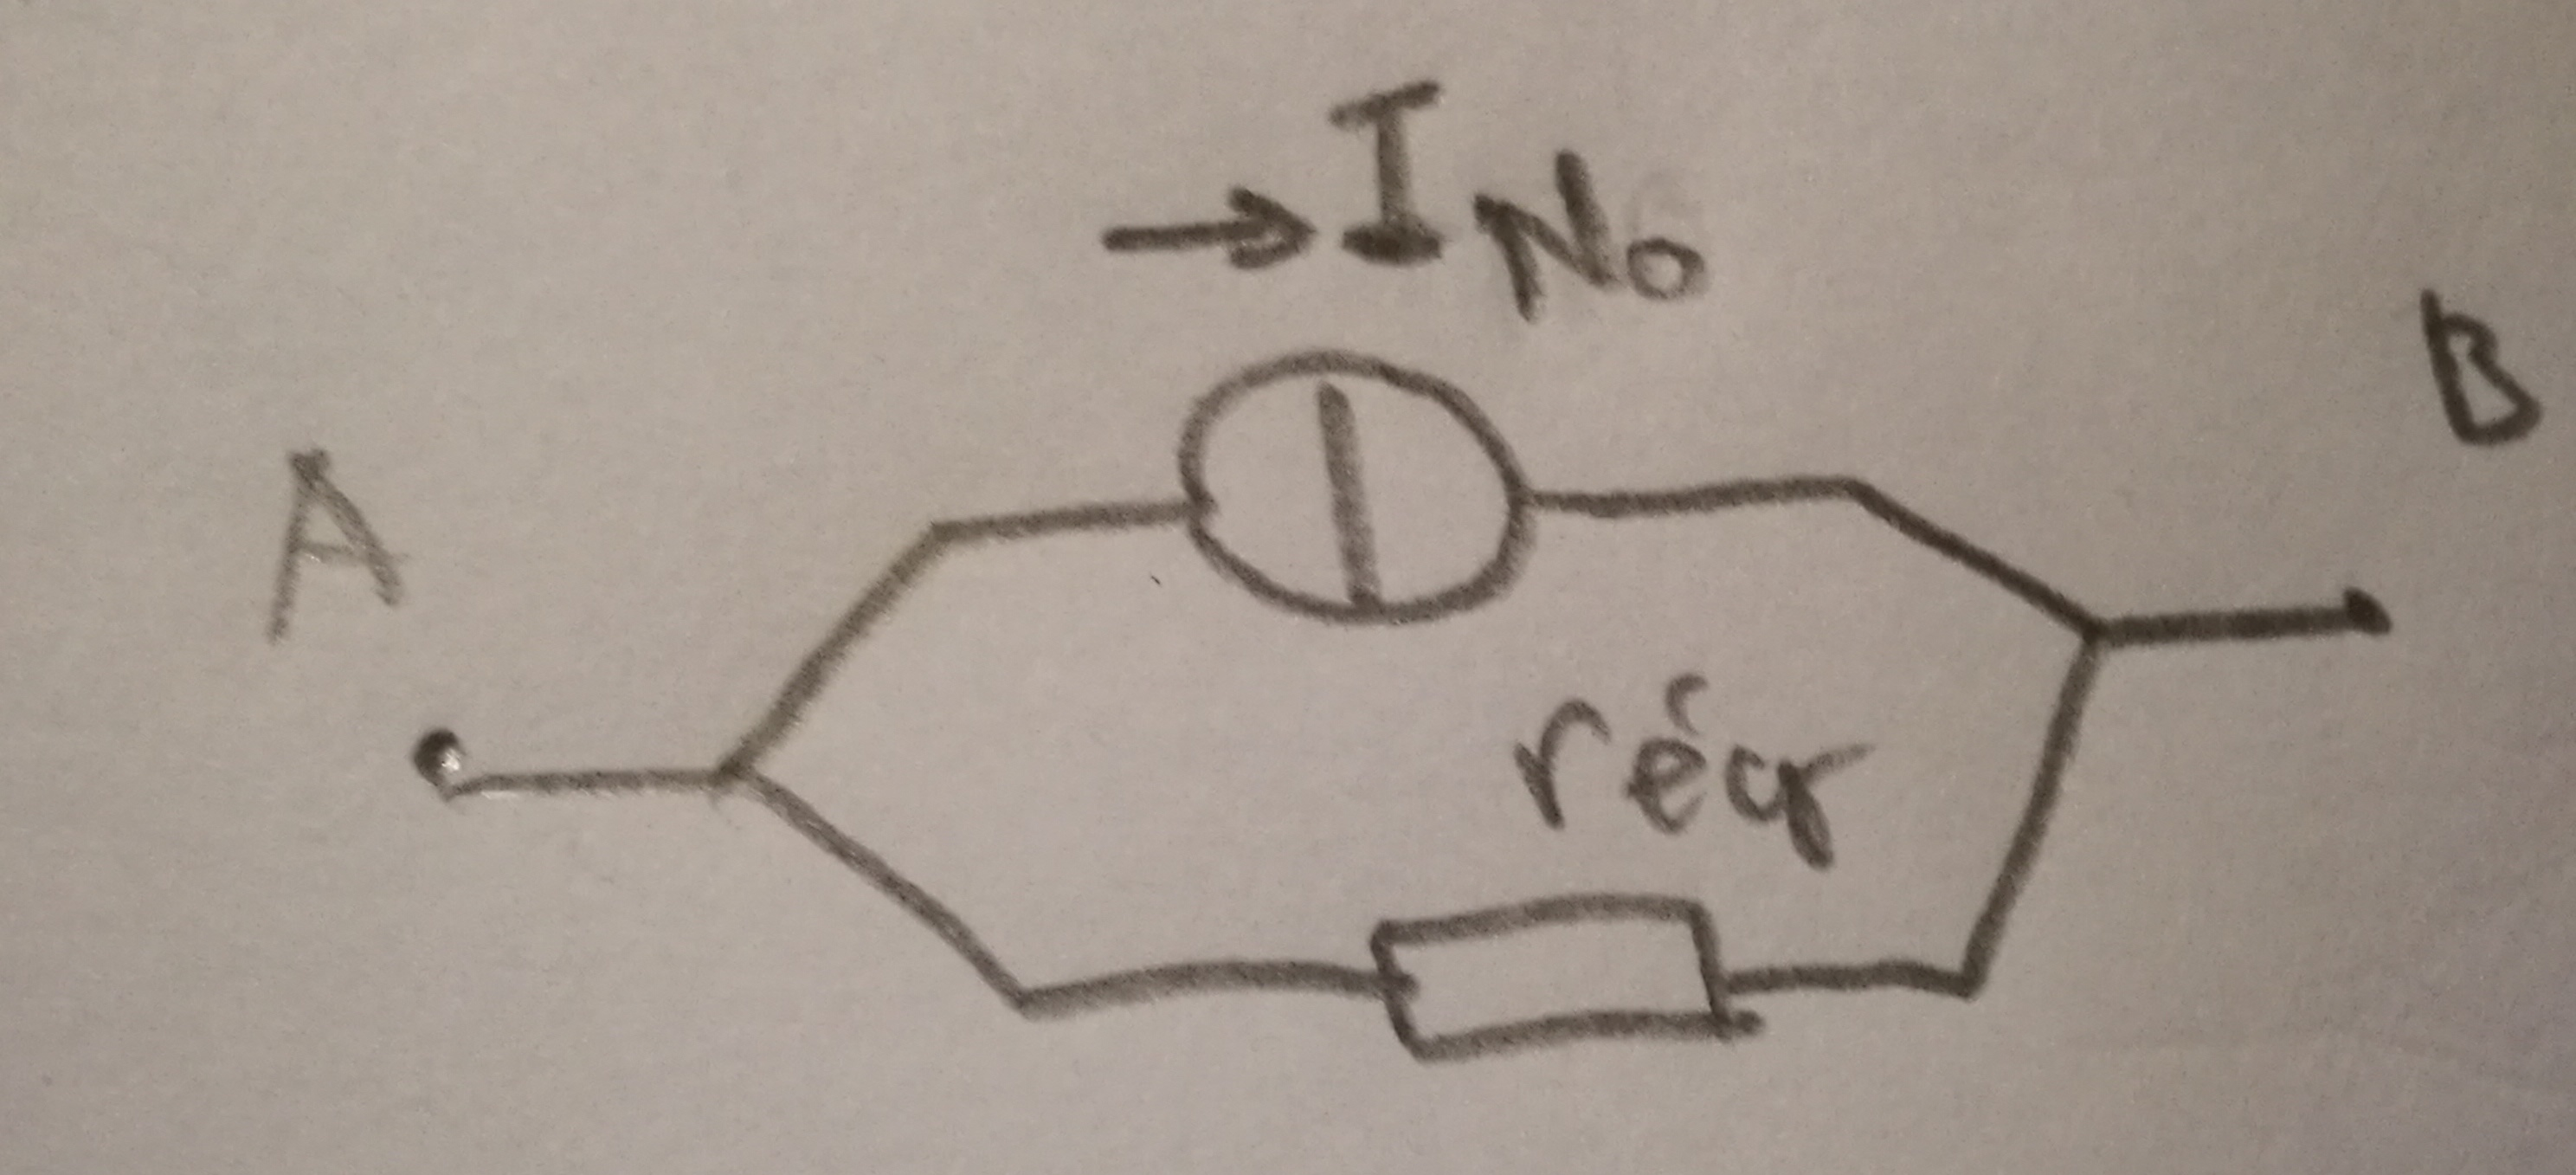
\includegraphics[scale=0.1]{Electrocinetique cadre et concepts de base//2}
\end{figure}


{\color{red} 二端有源原件可以等效为戴维南电源或诺顿电源} 

我们要做到等价一部分实际上是通过电学实验来从效果上确定的。比如我们如果要将原二端元件等价为戴维南电源,那么我们就可以从等价后的戴维南电源出发去寻找实验操作思路:

我要得到戴维南电源中的等效理想电压源的电压(即戴维南电压),就要断开A和B与外电路的联系(防止等效电阻分压),并连接电压表。这些操作要被移植到原二端元件上,并得到数据赋给戴维南电源元件

而对诺顿电源我们采取的操作是短路二端元件电路,此时理想电流源的电流不受影响,而等效电阻上没有了电流,这个操作同样要移植到原来的二端元件上.

而另一部分则是通过一系列对电路图的操作规则来确定的.%原理没想明白
在两个电路中我们确定等效电阻的方法都是通过把原电路中的理想电压源看成导线,理想电流源看成断开来得到一个“电阻图”,即为等效电阻的构成图。

{\color{red} 同一个二端元件等效出的戴维南电源和诺顿电源满足以下关系(用于两种电源的转换,经常会有这种需求):
$$r_{eq,Th}=r_{eq,No};\quad E_{Th}=I_{No}\cdot r_{eq}$$ } 

注意在等价时不要出现以下两种情况:

{\color{red}电压源不能并联},电压总会从高电压流低向电压,会造成低压源损坏,如果直接并联,电压高的会给电压低的充电,造成损坏。带上负载也只有电压高的在工作,但是电压源能串联,总电压等于2个电压相加 。

{\color{red}电流源不能串联},否则电流小的那个将被电流大的那个充电,造成损坏。但是电流源能并联,总电流等于2个电流相加。

\begin{figure}[H]
	\centering
	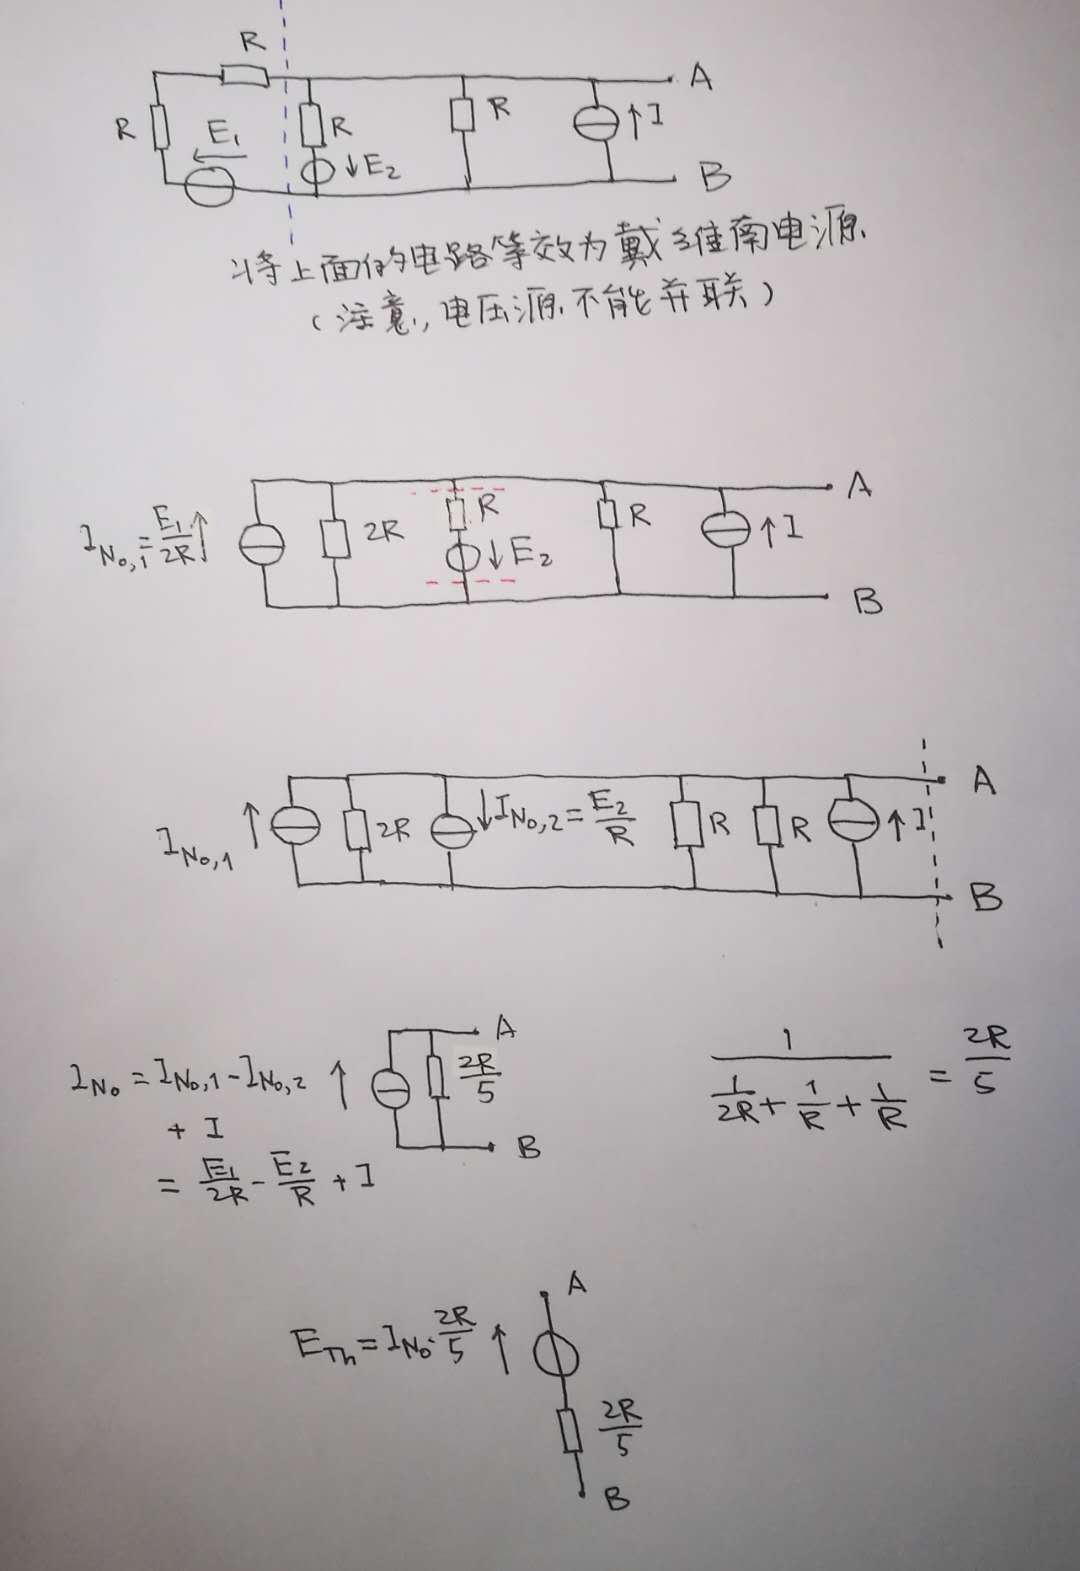
\includegraphics[scale=0.4]{Electrocinetique cadre et concepts de base//3}
\end{figure}
\textbf{注意初始的A,B两点可以看作一个完整回路的引出点.}



\section{求解电路的基本定律}
\paragraph{基尔霍夫定律}
\subparagraph{节点定律(Loi des nœud )}对一个节点处,流入的电流等于流出的电流(电荷守恒),或者所有流经该点的电流相加等于0,流入取正,流出取负。
\subparagraph{回路电压定律(Loi des mailles)}设定一个回路正方向,这一回路的电压根据正方向取正负号后,相加为零.

\chapter{Circuit linéaire du premier ordre}
\section{Exemple expérimental}
\subsection{Montage}
On cherche a observer, puis prévoir par le  calcul, le comportement du montage ci-dessous
lorsqu'il est alimenté par une tension constante délivrée par un générateur basss fréquence, nommé dans la suite par son acronyme GBF. On observe simultanément(同时) les tensions délivrées par le GBF et aux bornes du condensateur(电容器) sur les deux voies d'un oscilloscope(示波器).
\begin{figure}[H]
	\centering
	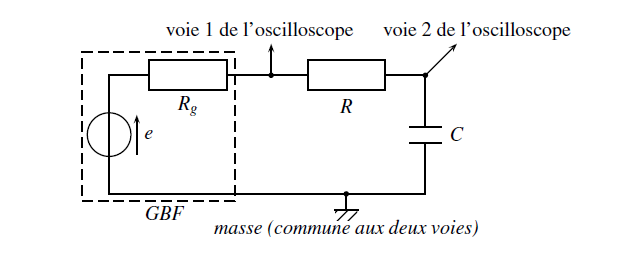
\includegraphics[scale=0.7]{Circuit lineaire du premier ordre//1}
\end{figure}

\section{暂态}
\textbf{分析流程:由元件特性做出初末态的等效电路图得到初末值;根据元件对应的欧姆定律得出微分方程;求解出对应的u,i和元件的值.}

\textbf{对于非电阻的元件,断路依旧可以有电压,短路依旧可以有电流}
\subsection{RC电路}
\paragraph{电容的欧姆定律}
$$
i_c=C\frac{du_c}{dt}
$$



\subsubsection{RC串联充电}
设置条件:初始电容器不带电,从而:

t=$0^-$时,开关未闭合 i($0^-$)=0 A,$u(0^-)$:=0 V

t=$0^+$时,\textbf{由于电荷是连续的,所以能量是连续的,对于电容器,$\mathit{E}$=$\frac{1}{2}Cu^2$,所以u连续是必要条件},
$u(0^+)=0$ V.\textbf{而此时根据电容"通交流阻直流"的特性,突然闭合开关使电路出现不稳定的交流状态,所以电路导通,又由于电容上此时电压为零,所以等效为导线(若初始电容带电则等效为这一时刻的恒定电压源)}

等效电路图为:
\begin{figure}[H]
	\centering
	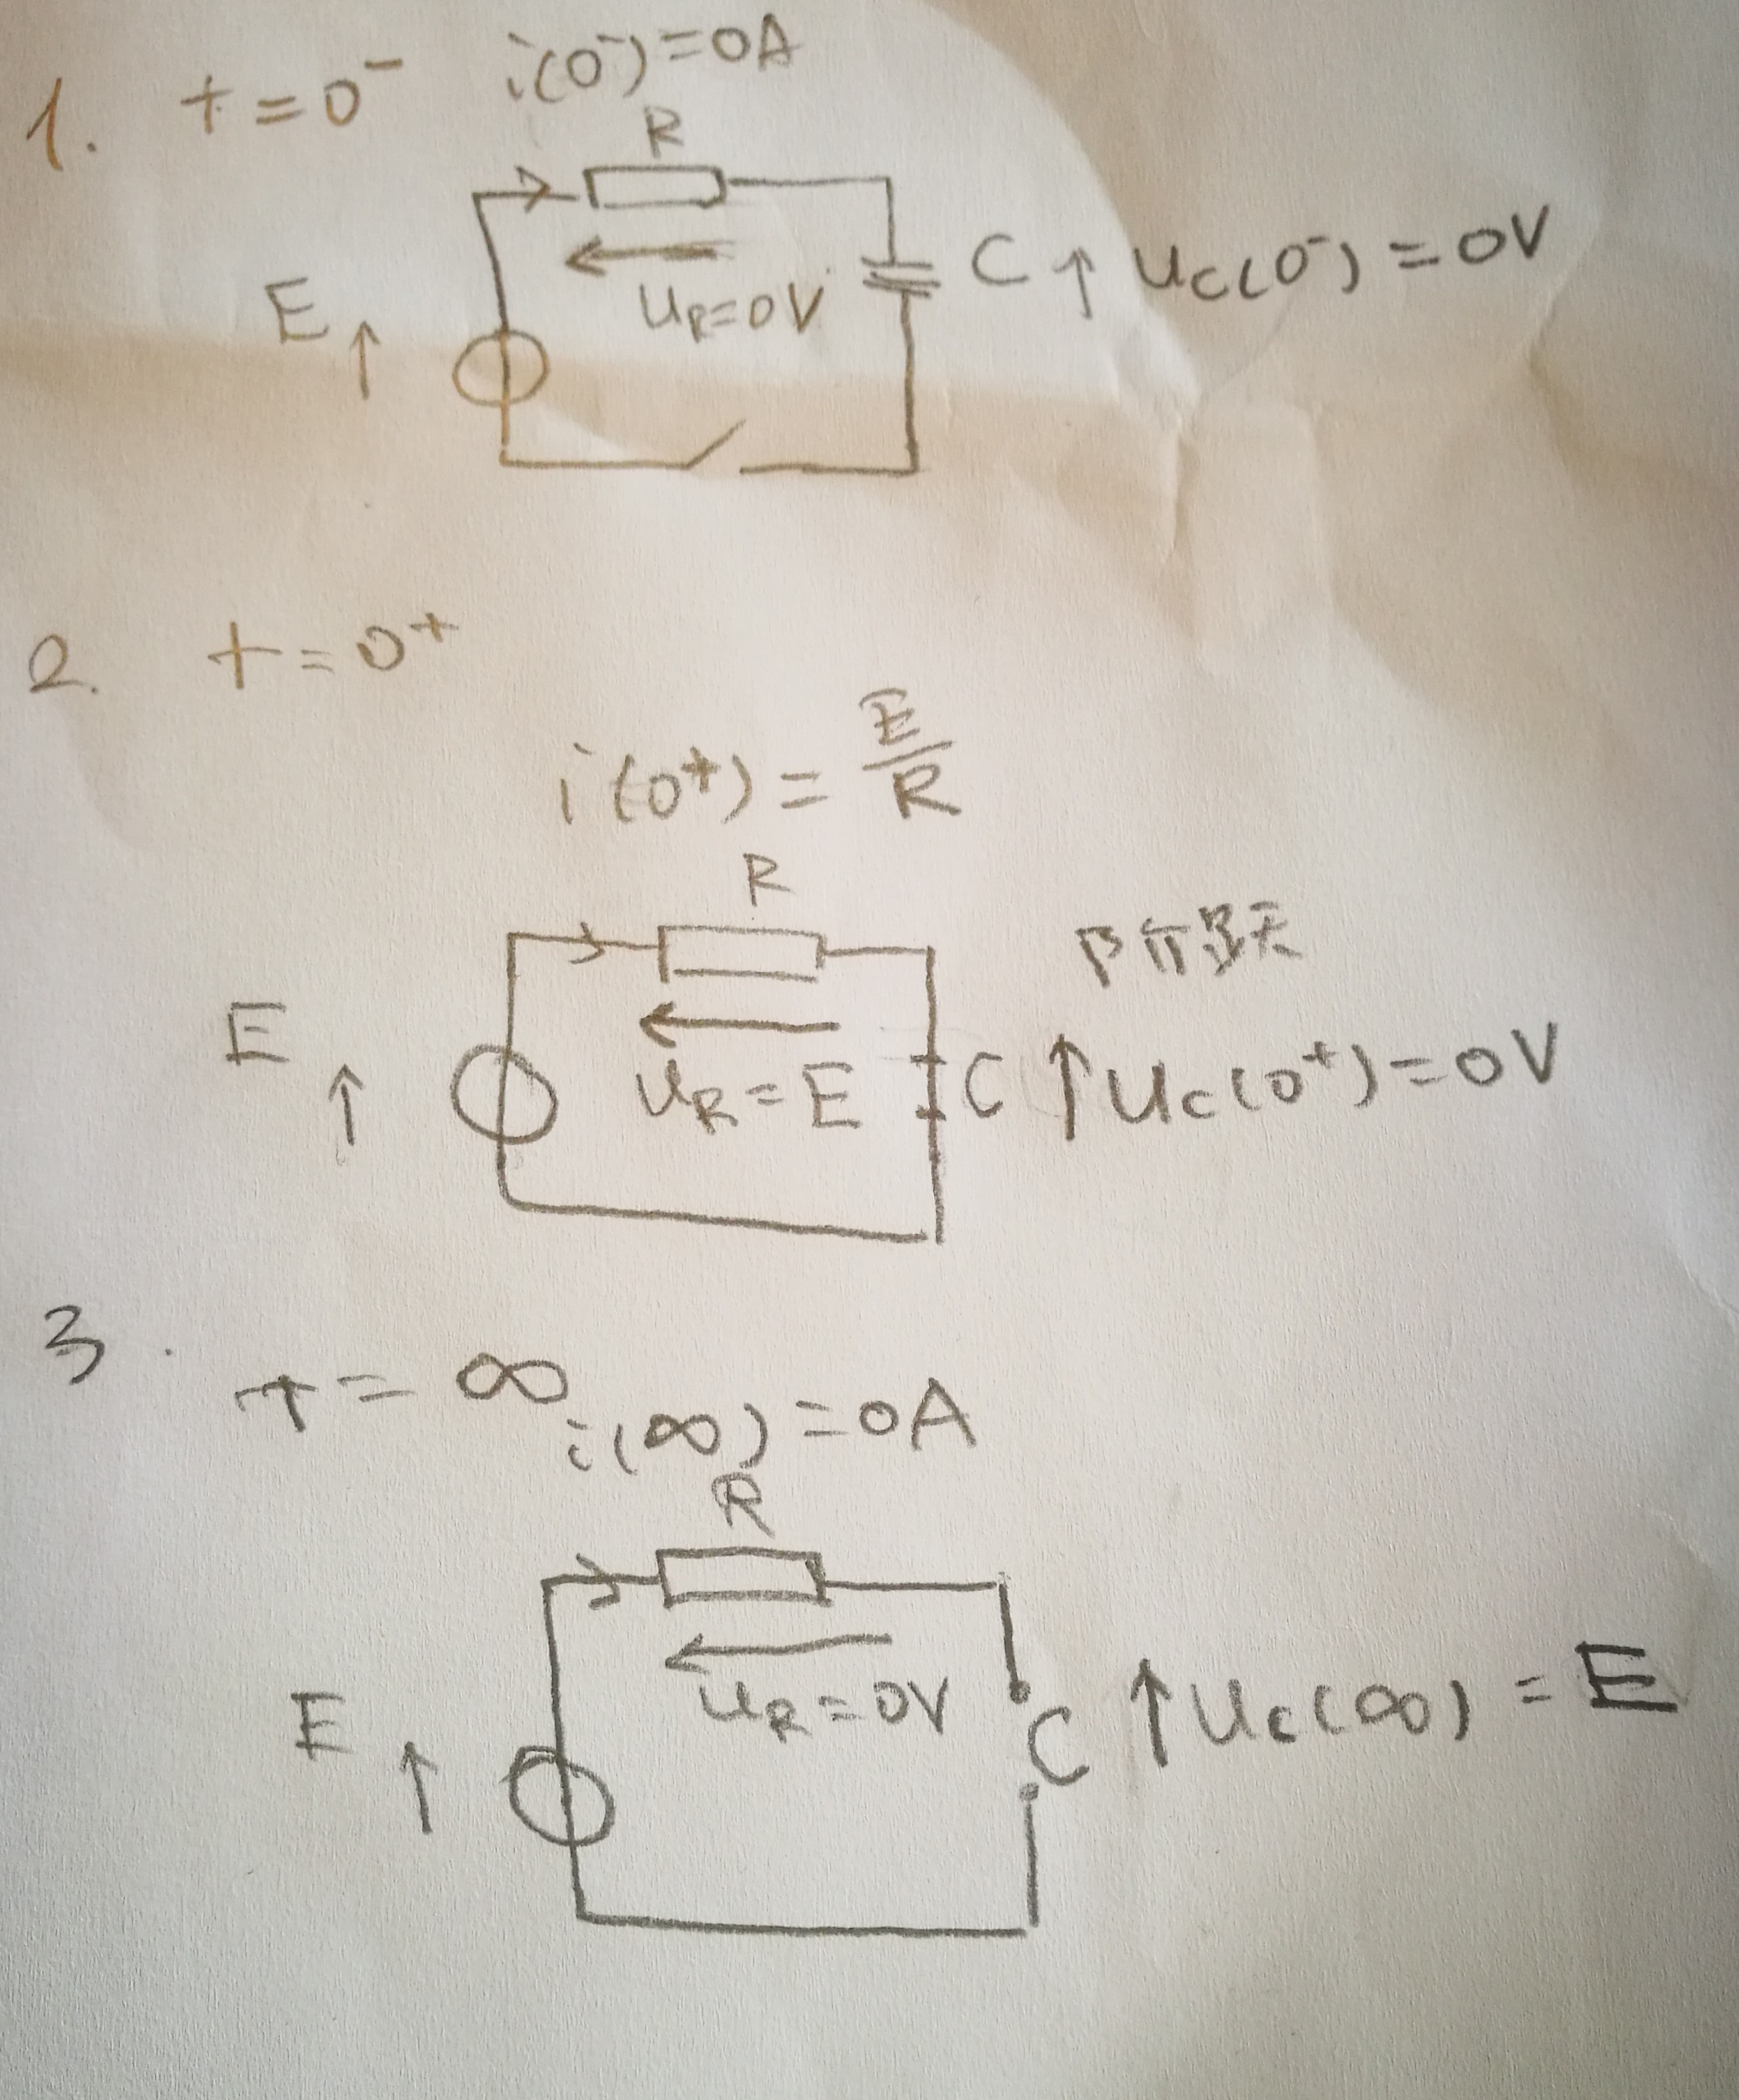
\includegraphics[scale=0.2]{Circuit lineaire du premier ordre//2}
\end{figure}

接下来取$t=0^+$到$\infty$中的任意一个时刻的电路图作为代表分析电路得到微分方程:
\begin{figure}[H]
	\centering
		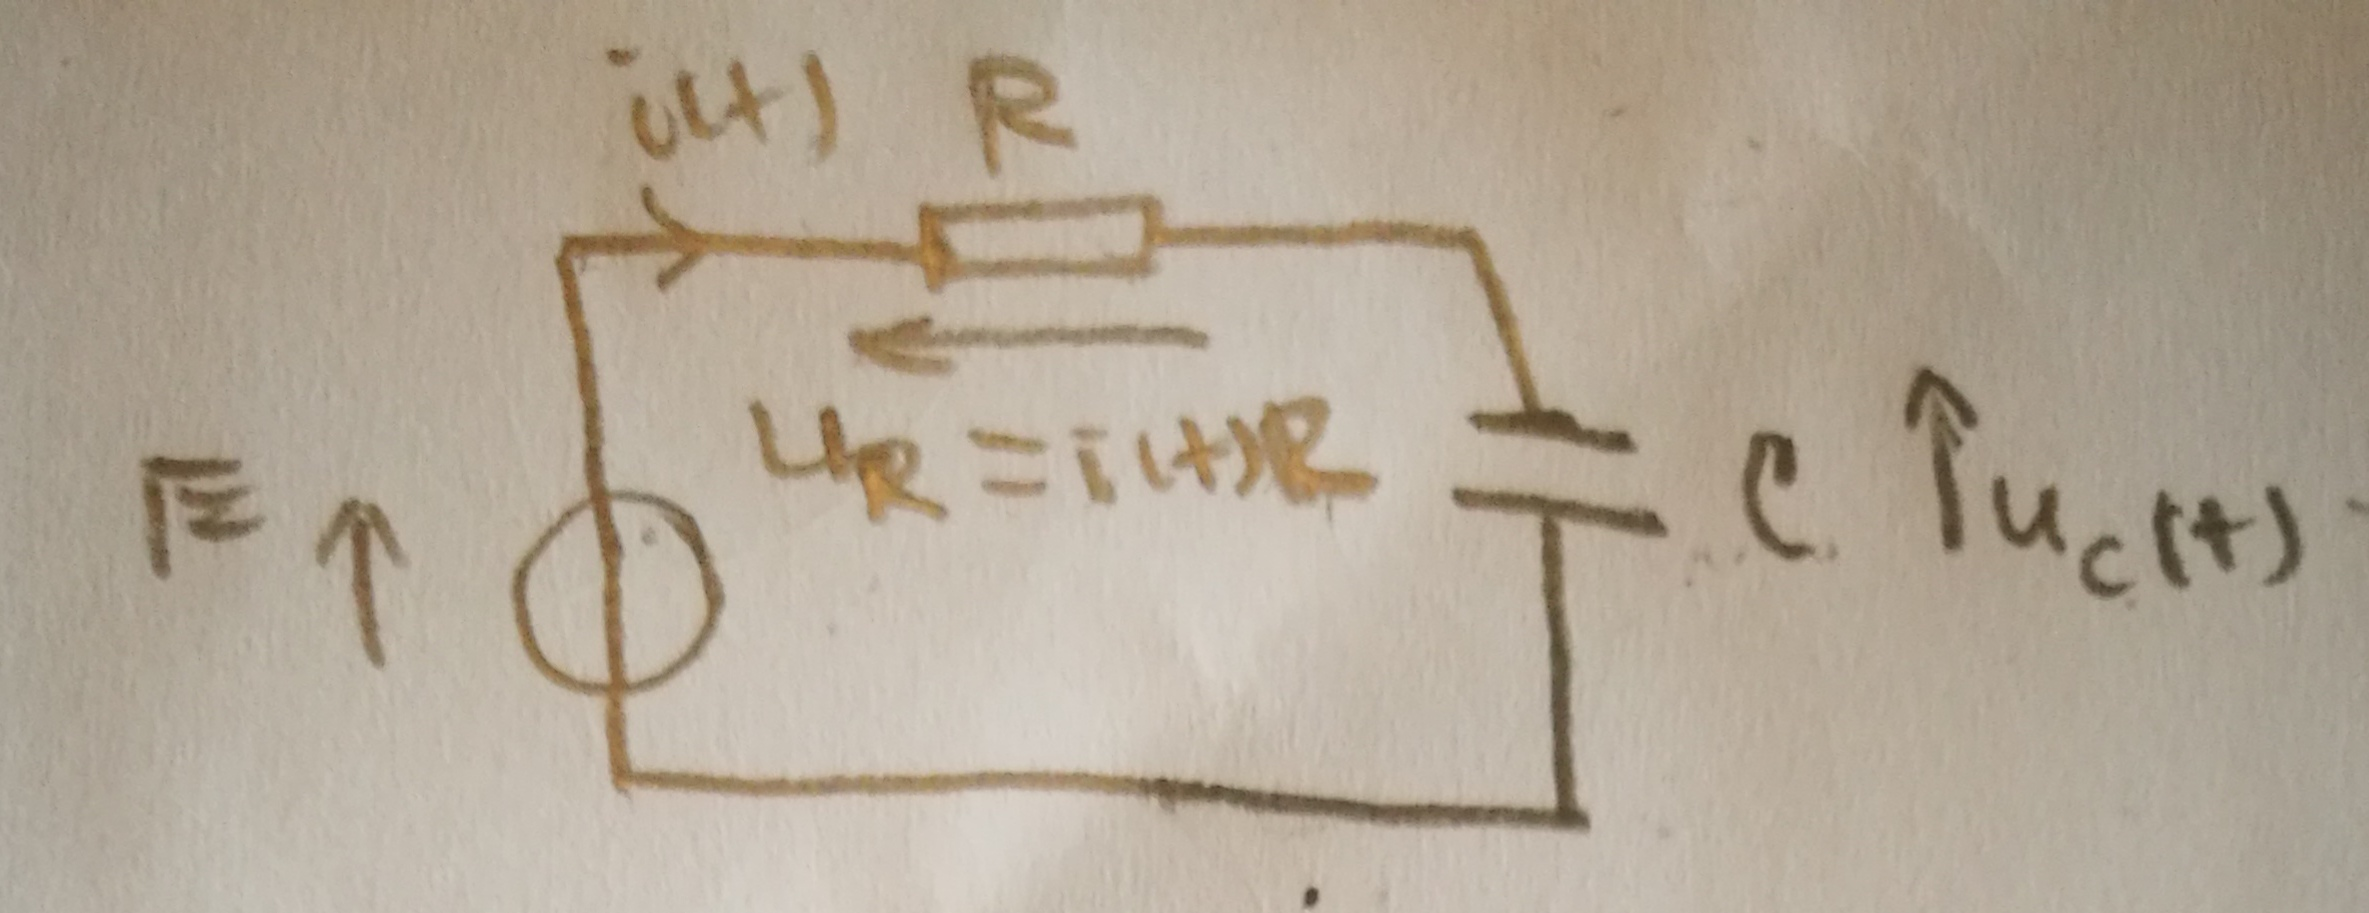
\includegraphics[scale=0.1]{Circuit lineaire du premier ordre//3}
\end{figure}


	$$E = i_cR+u_c$$
	$$E = RC\frac{du_c}{dt}+u_c$$
	$$
	\frac{E}{RC}= \frac{du_c}{dt}+\frac{u_c}{RC}
	$$

\chapter{Régime
	sinusoïdal forcé}

\textbf{Signal sinusoïdal}:

Considérons un signal $s(t)$ effectuant des oscillations sinusoïdales, noté: $s(t)=s_m\cos(\omega t+\phi)$
, avec $s_m>0$


\section{Représentation complexe du signal sinusoïdale}
Notons que l'amplitude de complexe $\underline{s_m}$ contient simultanément les informations
d'amplitude
$s_m$ et de phase $\phi$
de signal physique réel.

la representation de Fresnel de:$$
s(t)=s_m\cos(\omega t+\phi)
$$
est la représentation géométrique de son {\color{red}amplitude complexe} dans
le plan complexe.

我们来研究一下三角信号函数与其复数表示函数之间的运算关系。先来说一个概念:“线性运算”。线性运算包括:线性组合,微分运算和积分运算。复数表示可以作为déterminer线性运算的一个工具,但La représentation complexe ne
permet pas de déterminer le produit
de deux fonctions sinusoïdales.下面我们就来看看验证关于三件事的说法:1.求导;2.积分;3.函数积。

\paragraph{Dérivation}

对三角信号$s(t)=s_m\cos(\omega t + \phi)$求导,我们得到:
$$
\frac{\mathrm{d} s(t)}{\mathrm{d}t}=-\omega s_m\sin (\omega t + \phi)=\omega s_m\cos (\omega t + \phi+\frac{\pi}{2})
$$

Dériver sa représentation complexe $\underline{s}(t)$ est simple
$$
\frac{\mathrm{d} \underline{s}(t)}{\mathrm{d}t}=j\omega\underline{s}_me^{j\omega t}=j\omega\underline{s}(t)
$$
注意到:
$$
\mathcal{R}e(\frac{\mathrm{d} \underline{s}(t)}{\mathrm{d}t})=\mathcal{R}e(j\omega\underline{s}(t))=\mathcal{R}e(s_me^{\omega t +\phi+\frac{\pi}{2}})=\frac{\mathrm{d} s(t)}{\mathrm{d}t}
$$

\paragraph{Intégration: primitive sinusoïdale}Intégrons le signal sinusoïdal en restant dans le domaine des signaux oscillants, \textbf{de
valeur moyenne nulle}.Ainsi, nous associons au signal $s(t)=s_m\cos(\omega t + \phi)$
sa primitive sinusoïdale (constante d'intégration nulle)
$$
S(t)=\frac{s_m}{\omega}\sin(\omega t+\phi)=\frac{s_m}{\omega}\cos(\omega t +\phi-\frac{\pi}{2})
$$
Intégrer de la même façon sa représentation complexe $\underline{s}(t)$ revient simplement
à poser:
$$
\underline{S}(t)=\frac{\underline{s}_m}{j\omega}e^{j\omega t}=\frac{\underline{s}}{j\omega}
$$

et nous vérifions que :
$$
\mathcal{R}e(\underline{S}(t))=\mathcal{R}e(\frac{\underline{s}}{j\omega})=\mathcal{R}e(\frac{\underline{s}_m}{\omega}e^{j\omega t-\frac{\pi}{2}})=\mathcal{R}e(S(t))
$$

Les opérations de dérivation et intégration de la représentation complexe
d'un signal sont très simples puisqu'il suffit de multiplier ou diviser,
respectivement, le signal complexe par le facteur $j\omega$.

\paragraph{三角信号函数乘法}Considérons en effet deux signaux
sinusoïdaux :
$$
s_1(t)=s_{1m}\cos(\omega t +\phi_{1})
$$
$$
s_2(t)=s_{2m}\cos(\omega t +\phi_{2})
$$
我们有根据三角函数积化和差:
$$
s_1(t)s_2(t)=\frac{1}{2}s_{1m}s_{2m}(\cos(2\omega t +\phi_{1}+\phi_{2})+\cos(\phi_{1}-\phi_{2}))
$$

Le produit des représentations
complexes est :
$$
\underline{s}_1(t)\underline{s}_2(t)=s_{1m}s_{2m}e^{2\omega t +\phi_{1}+\phi_{2}}
$$
它的实部为:
$$
\mathcal{R}e(\underline{s}_1(t)\underline{s}_2(t))=
s_{1m}s_{2m}\cos(2\omega t +\phi_{1}+\phi_{2}) 
$$
Il est clair que :
$$
\mathcal{R}e(\underline{s}_1(t)\underline{s}_2(t))\not =
s_1(t)s_2(t)
$$
\section{Utilisation du plan complexe}

Déterminer pour le nombre complexe $\underline{z}=1-x^2+j\frac{x}{Q}$
, le module $z$ , l'argument $\phi$ et la courbe
$(C)$ décrite quand la variable réelle $x$ varie de zéro
à l'infini ($Q$ est une constante réelle positive)

En élimant $x$ entre $X=1-x^2$ et Y=$\frac{x}{Q}$ nous
obtenons l’équation de la demi-parabole $(C)$ décrite
par l'image $M$ de $\underline{z}$ :
$$
X=1-Q^2Y^2
$$ , avec $Y\ge 0$
.Le module de $\underline{z}$ est :
$$
z=\sqrt{(1-x^2)^2+(\frac{x}{Q})^2}
$$
et son argument :
$$
\phi=\left\{
\begin{aligned}
\arctan{[\frac{x}{Q(1-x^2)}]}&\quad \text{si} \quad(1-x^2)\ge 0;\\
\pi+\arctan{[\frac{x}{Q(1-x^2)}]}&\quad \text{si} \quad (1-x^2) < 0.\\
\end{aligned}
\right.
$$

\begin{figure}[H]
	\centering
	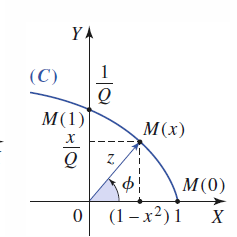
\includegraphics[scale=1]{Regime sinusoidal force//1}
\end{figure}
注意$\arctan$对应角在]-$\frac{\pi}{2}$,$\frac{\pi}{2}$[之间。
\section{Puissance moyenne–Facteur de puissance}
Notons par $i(t)=i_m\cos(\omega t+\phi_{i})$ le courant traversant le dipôle, et la tension
à ses bornes par $u(t)=u_m\cos(\omega t+\phi_{u})$
L'expression de la puissance instantanée s'écrit :
$$
p(t)==u_m\cos(\omega t+\phi_{u})i_m\cos(\omega t+\phi_{i})=\frac{u_mi_m}{2}[\cos(\phi_{u}-\phi_{i})+\cos(2\omega t+\phi_{u}+\phi_{i})]
$$
Elle comporte deux termes:
\begin{itemize}
\item $\mathfrak{P}=\frac{u_mi_m}{2}\cos(\varphi)$,avec
$\varphi=\phi_{u}-\phi_{i}$ déphasage de la tension par rapport au courant. C'est un terme constant ;
\item $\frac{u_mi_m}{2}\cos(2\omega t+\phi_{u}+\phi_{i})$, terme sinusoïdal de fréquence double de celle des signaux $u(t)$ et $i(t)$. Sa valeur moyenne est nulle.
\end{itemize}
En conséquence, la puissance moyenne a pour expression :
$$
\mathfrak{P}=\frac{u_mi_m}{2}\cos(\varphi)
$$
En régime harmonique, la puissance moyenne est appelée puissance active. Elle s'exprime en watt (symbole : W).
\begin{figure}[H]
	\centering
	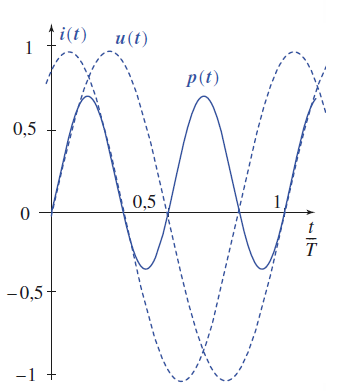
\includegraphics[scale=1]{Regime sinusoidal force//2}
\end{figure}
平均功率其实是一个包含了电流和电压的振幅信息和相位差信息的“宝藏”。


















\chapter{Étude du circuit RLC série-Résonances}
Nous nous intéresserons désormais à la seule réponse sinusoïdale, le régime
transitoire ayant disparu plus ou moins rapidement.

词义解释:\\
\textbf{Résonance: augmentation de l'amplitude d'oscillation d'un système,sous l'influence d'impulsations régulières de fréquence voisine de la fréquence propre du système}

谐振其实是概括了一种现象:即在{\color{red}频率接近系统本征频率}的规则脉冲(在这里可以理解为输入的电源信号)的影响下,系统的振荡信号的振幅增加。不过这是对整个系统而言的信号(如整个电路的i)的谐振的定义,对于单个元件,我们有另外一种我认为是对名词的一种abuse("滥用")的“谐振的定义”:当输入信号的频率接近一个频率(可能不是系统本征频率,而是一个固定的,由系统特征量($\omega_0$,Q)组合而成的频率)时,该元件两端的电压(如我们将看到的电容两端的电压)达到极大值。

我们研究的对象是一个RLC电路
\begin{figure}[H]
	\centering
	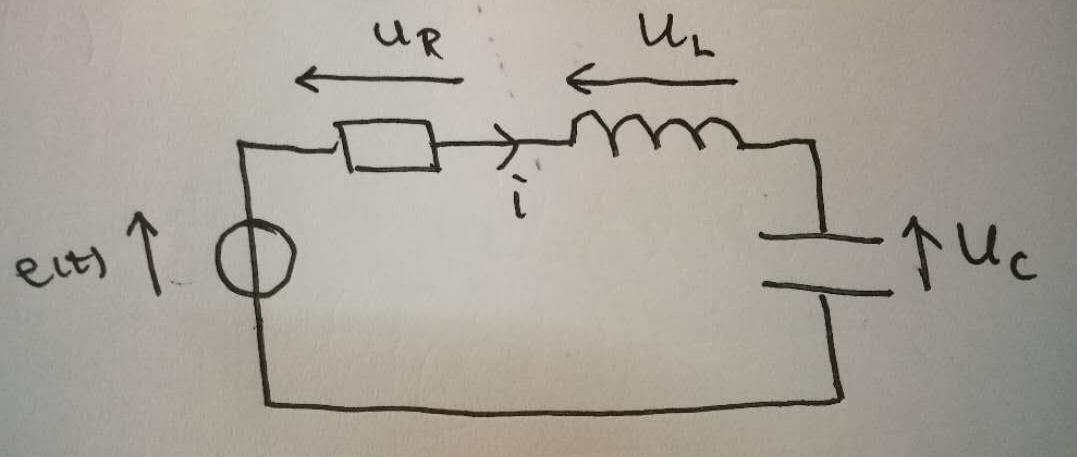
\includegraphics[scale=0.2]{Etude du circuit RLC serie-Resonances//1}
\end{figure}
我们想要通过从低到高调整电源电压函数频率的方式(即“扫频”)来观察并研究对应的电路中的一些元件两端的电压函数的振幅和这些电压函数与电源输入的电压函数之间相位差的变化情况。(动机是验证谐振现象的两个关键描述:振幅最大和输入频率接近本征频率)

\section{电流的谐振}
我们先来看看扫频的实验现象(这里我们看$u_R$两端的电压(看电压是因为示波器测的是电压信号)就可以反映电流的幅值变化和与电源电压的相位差变化)
\begin{figure}[H]
	\centering
	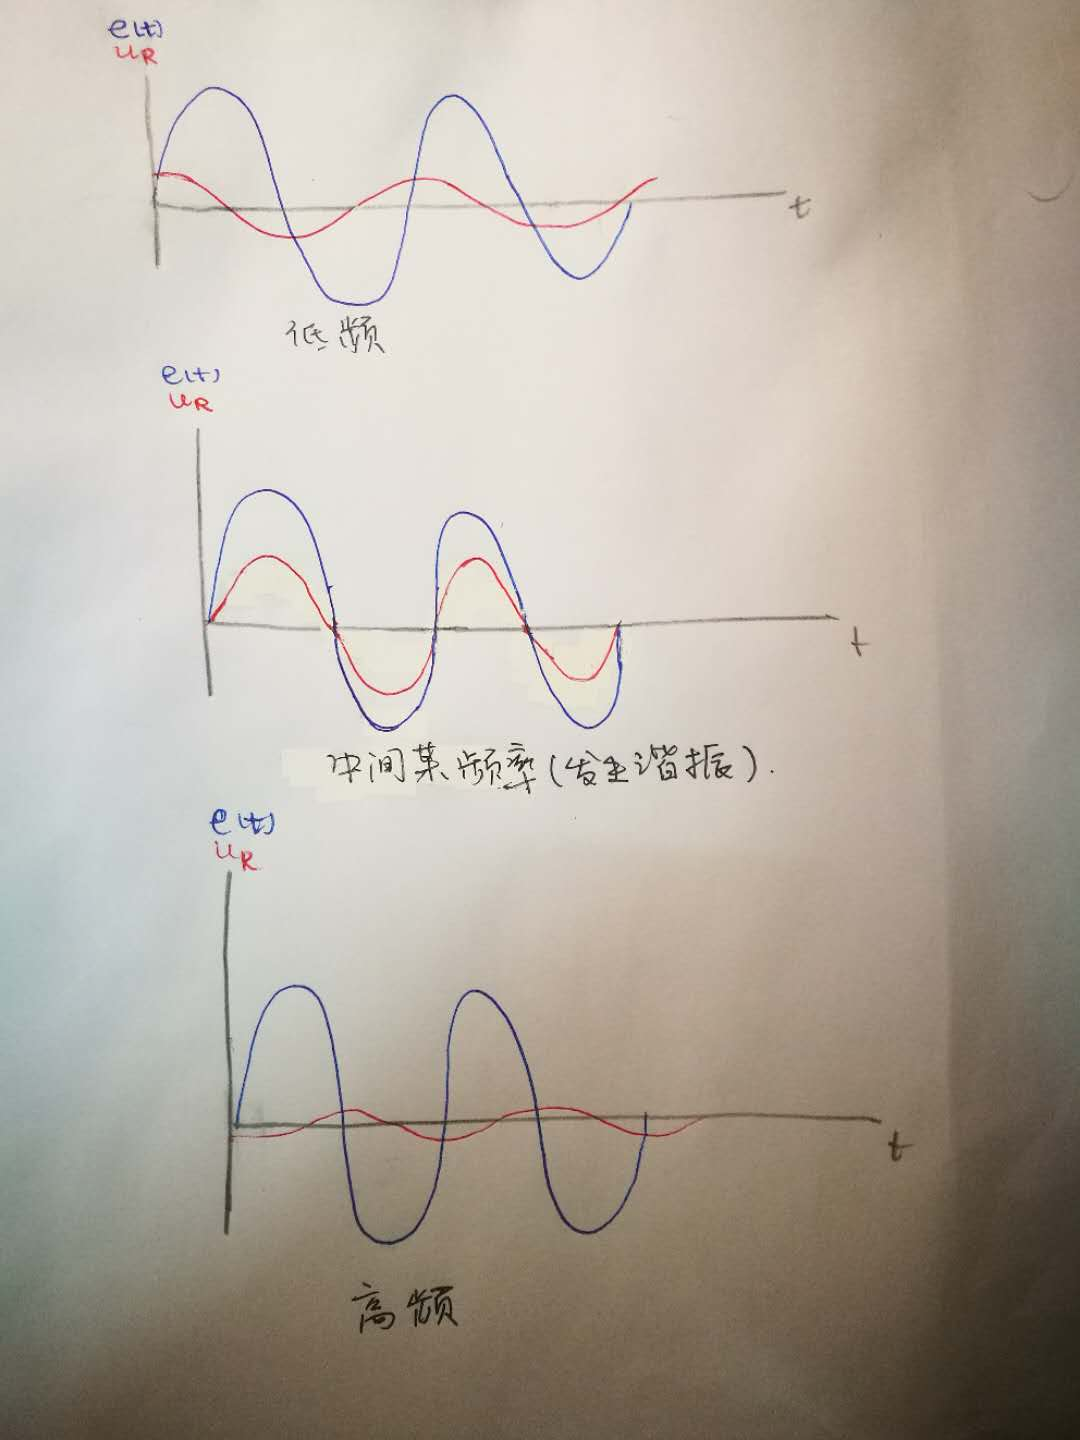
\includegraphics[scale=0.2]{Etude du circuit RLC serie-Resonances//2}
\end{figure}
\subsection{得到电流的复振幅关于约化角频率的函数}
在具体的研究振幅和相位差的问题之前,我们需要在此处认清几个概念.
\begin{itemize}

\item 首先,相位差的究竟是指谁相对于谁的相位差,是否有convention可以指导我们从语境中确定这一点?这其实又是一个语言abuse:当我们说到A与B的相位差时我们指的是A的相位减去B的相位(也就是A{\color{red}提前}于B多少相位),一般记为$\phi_{A/B}$,若$\phi _{B}=0$,我们也可以就把$\phi_{A/B}$记为$\phi_{A}$(这里$\phi_{A}$与$\phi_{B}$分别指A,B相对于零相位的相位差)另外,当我们提到相位差时,往往又会有另一个东西来混淆我们的认知,那就是迟滞时间,(讨厌的是这个概念是我们计算$\phi_{A/B}=\phi_{A}-\phi_{B}$时不能回避的点),当我们说A相对于B{\color{red}落后}多少时间时,我们说的是A对B的迟滞时间:$\Delta t=t_B-t_A$(这里$t_A$与$t_B$的定义分别是A,B相对于时间原点的迟滞的时间)两个量的关系是:
$$
\phi_{A/B}=-\omega \Delta t
$$

为简化研究,我们下面把电源电压的相位设为零相位
\item 然后我们需要复振幅的概念(这意味着我们需要用到复数表示):复振幅虽然像是振幅但实际上包含了我们需要研究的两个要素:振幅和相位

\item 为了得出RLC电路的特征量和电流的复振幅,我们得先建立关于电路关于电流的微分方程:

由回路定理,$u_R+u_L+u_C=e(t)$
,即$L\frac{\mathrm{d} i}{\mathrm{d} t} + Ri + u_C = e(t)$,利用电容特性,将电压$u_C$转化为电流,需要对方程整体关于时间再求一次导:
L$\frac{\mathrm{d^2} i}{\mathrm{d} t^2} + R\frac{\mathrm{d} i}{\mathrm{d} t}+\frac{i}{C}=\frac{\mathrm{d} e}{\mathrm{d} t}$
转化为标准形式:
$$
\frac{\mathrm{d^2} i}{\mathrm{d} t^2} + \frac{R}{L}\frac{\mathrm{d} i}{\mathrm{d} t}+\frac{i}{LC}=\frac{1}{L}\frac{\mathrm{d} e}{\mathrm{d} t}
$$
\begin{itemize}
	
\item 电路特征量的定义式:
$$
\frac{\mathrm{d^2} i}{\mathrm{d} t^2} + \frac{\omega_0}{Q}\frac{\mathrm{d} i}{\mathrm{d} t}+{\omega_0}^2 i=0
$$
从而对应出:
$$
{\omega_0}^2=\frac{1}{LC}
$$
$$
\frac{\omega_0}{Q}=\frac{R}{L}
$$

\item 复数表示下的求导:
把上面的微分方程中的$i$和$e$两个函数换成复数表示,
$\underline{i}=\underline{I}e^{j\omega t}$,
$\underline{e}=\underline{E}e^{j\omega t}$其中$\underline{I}$
和$\underline{E}$都是常复数,求导过程中保留不变,而对于$e^{j\omega t}$这一项,则每求一次导多出一个$j\omega$的系数
所以方程
$$
\frac{\mathrm{d^2} \underline{i}}{\mathrm{d} t^2} + \frac{\omega_0}{Q}\frac{\mathrm{d} \underline{i}}{\mathrm{d} t}+{\omega_0}^2 i=\frac{1}{L}\frac{\mathrm{d} \underline{e}}{\mathrm{d} t}
$$
变成
$$
(j\omega)^2\underline{i}+j\omega\frac{\omega_0}{Q}\underline{i}+
{\omega_0}^2 \underline{i}=j\omega\frac{1}{L}
\underline{e}$$
这时候就没有必要保留函数部分了,直接两边约掉$\underline{i}$和$\underline{e}$中的$e^{j\omega t}$部分,只留下复振幅,我们再化简一下得到$i$的复振幅的表达式:
$$
\underline{I}=\frac{j\omega\underline{E}/L}{-\omega^2+j\omega\frac{\omega_0}{Q}+{\omega_0}^2}
$$
\item 我们引入约化角频率(la pulsation réduite)$x=\frac{\omega}{\omega_0}$来改写上面的表达式
上下同时约去${\omega_0}^2$我们得到
$$
\underline{I}=\frac{jEx/(\omega_0{\color{red}L})}{-x^2+j\frac{x}{Q}+1}
$$
然后上下同时乘上$-jQ/x$,并根据
$$Q/(\omega_0L)=1/R$$
得到:
$$
\underline{I}=\frac{E/R}{jQx+1-jQ/x}=\frac{E/R}{1+jQ(x-1/x)}
$$
\end{itemize}
\end{itemize}

现在,我们已经通过前期准备,得到了
包含我们想要研究的谐振现象两大要素的复振幅$\underline{I}$。

\subsection{振幅与相位差关于约化角频率的函数图像}
振幅的信息包含在复振幅中,它是复振幅函数的模,
$$
I=\frac{E/R}{\sqrt{1+(Q(x-1/x))^2}}
$$
同样相位差的信息也包含在复振幅中,
(注,严格地说应该是相位的信息包含在复振幅中,但这里因为取$e$的相位为零相位,所以$i$的相位就是$i$与$e$的相位差)
$$
\phi_{i}=k\pi-\arctan{Q(x-1/x)}
,\quad k\in \llbracket -1, 1 \rrbracket$$
注意$\phi_{i}$实际上是由下式推出的:
$$
\phi_{i}=\text{分子的幅角$-$分母的幅角}=0-\text{分母的幅角}
$$
这里分母的幅角实际上是下面的一个方程的解
$$
\tan(\text{分母的幅角})=Q(x-1/x)
$$
这个方程的解本应是:
$$
\text{分母的幅角}=k'\pi+\arctan{Q(x-1/x)},\quad k'\in \mathbb{Z}
$$
但是由于相位差只能被限制在$[-\pi,\pi]$的区间内(超过这个区间就会出现两种比较方式,两个图像之间的提前落后关系就会出现两种结果,造成含混),所以k只能取$ \llbracket -1, 1 \rrbracket$之间的值。

$\arctan$这个函数,它定义域为$\mathbb{R}$,周期为$\pi$,然而值域为$]\frac{-\pi}{2},\frac{\pi}{2}[ $
,所以要先确定相位差的范围,才能确定$\phi_{i}$的表达式中的k的取值。这就需要下面的对渐进行为的研究。


在低频时,由于此时电容的复阻抗趋于无穷,电感的复阻抗趋于0,故我们将电容视为断开的开关,电感视为导线;在高频时则相反,电容视为导线,电感视为断开的开关。等效电路图如下所示
\begin{figure}[H]
	\centering
	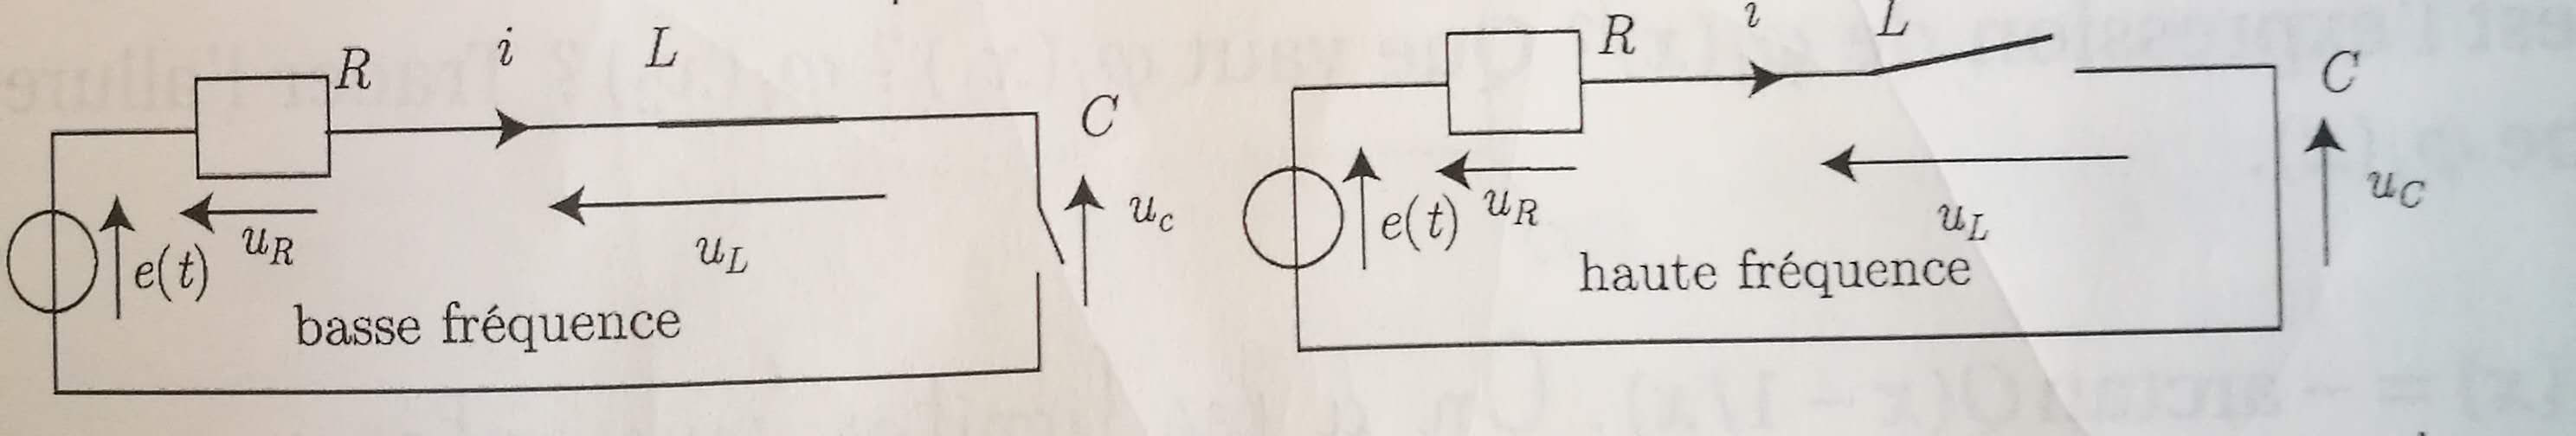
\includegraphics[scale=0.15]{Etude du circuit RLC serie-Resonances//3}
\end{figure}
我们有$i_0\approx 0$ 及$i_{\infty}\approx0$,对于相位差,我们需要根据等效电路图做出Fresnel表示:

我们先交代如何在Fresnel图中表示出相位差:首先我们要确定一个参考方向轴(如下图中的$\underline{i}$),这个可以只起方向参考的作用而不用管模长是否符合实际,然后我们要通过已知的相对参考方向相位差和相对模长作出已知向量($\underline{u_R}$,$\underline{u_L}$.$\underline{u_C}$),最后由矢量合成得到我们需要的向量($\underline{e}$),然后相位差就是二者对应向量的夹角,方向从减数对应的向量指向被减数对应的向量,符号取逆时针为正。
\begin{figure}[H]
	\centering
	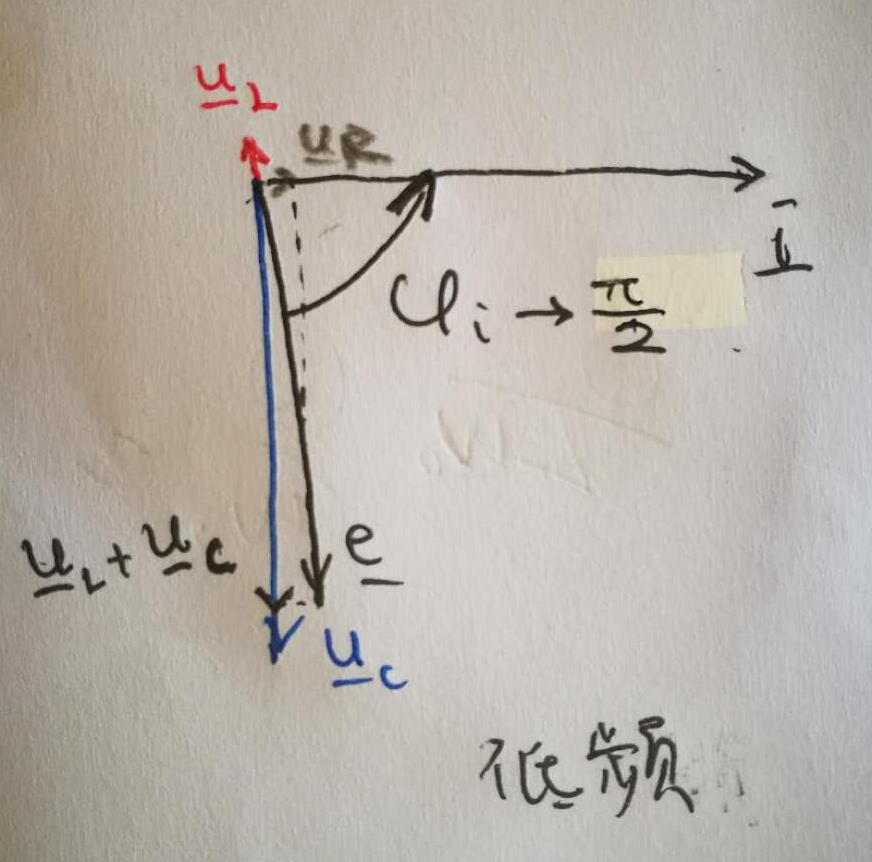
\includegraphics[scale=0.2]{Etude du circuit RLC serie-Resonances//4}
\end{figure}

\begin{figure}[H]
	\centering
	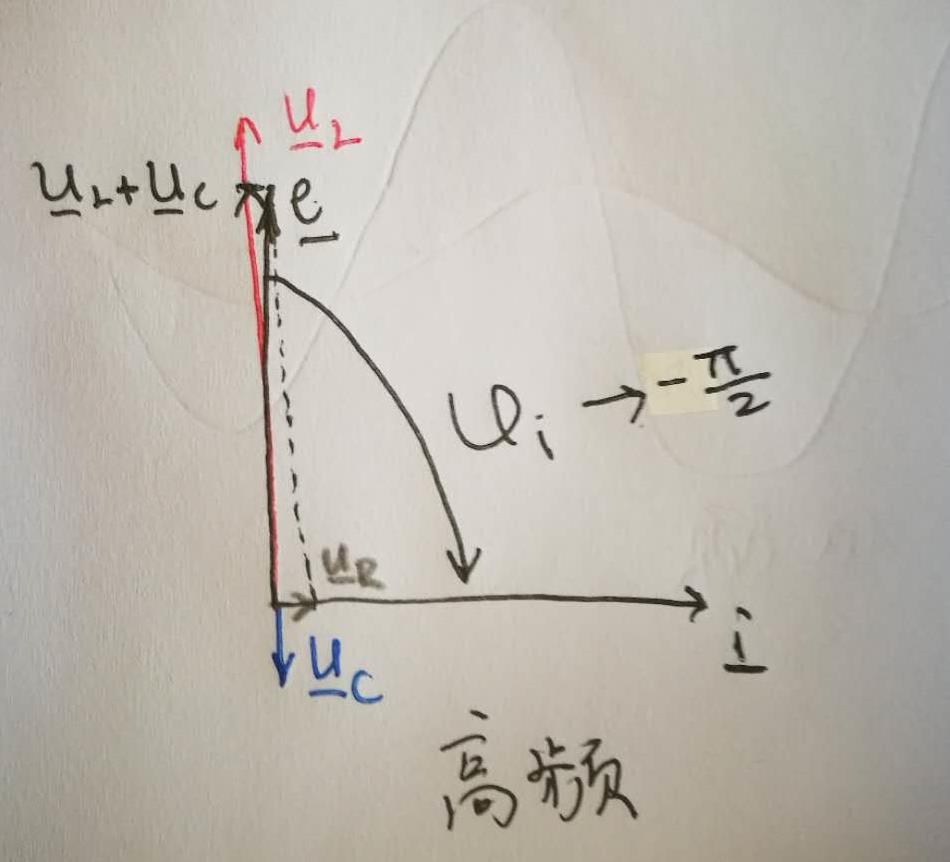
\includegraphics[scale=0.2]{Etude du circuit RLC serie-Resonances//5}
\end{figure}
由上图可知$\phi_{i}\in ]\frac{-\pi}{2},\frac{\pi}{2}[$,所以$\phi_{i}$的表达式中$k=0$。

下面我们来验证一下谐振现象,看看数学上给出的解释是否符合现象,为此我们先来看一下振幅在什么条件取极大值。$I$在$x-1/x=0$的时候取到最大值,此时$x=1$(注意,根据$x$的物理意义,$x>0$),我们有:
$$
x_r=1
$$
$$
w_r=w_0
$$
$$
I_{max}=E/R
$$
$$
\phi_{i,r}=0
$$
\quad \quad \quad \quad \quad \quad \quad \quad \quad \quad \quad \quad (角标r代表résonance)

注意上面的$\phi_{i,r}=0$是可以通过Fresnel图来得到的,不过思路跟用Fresnel图得出相位差时有些不一样:

这回$\underline{u_R}$,$\underline{u_L}$,$\underline{u_C}$之间的模长的相对大小无法确定,只有相对位置是确定的,这时,$\underline{e}$的模长我们可以确定下来,但是与$\underline{i}$之间的夹角不确定。

由于($\underline{u_R}$,$\underline{u_L}$.$\underline{u_C}$)的矢量合为$\underline{e}$,且$\underline{u_R}$的方向在一条确定的射线上,$\underline{u_R}$与$\underline{u_L}$的矢量合在另一条确定的直线上,这样我们只需要观察$\underline{e}$在变动与$\underline{i}$之间夹角的过程中,在$\underline{u_R}$的方向上投影的最大值即可(此时$\underline{u_R}$最大意味者$\underline{i}$最大)。我们很容易得出结论:当$\underline{e}$全部投影在
$\underline{u_R}$方向上时显然投影最大,此时,$\phi_{i}=0$.

下面我们会具体地画出$I(x)$和$\phi_{i}(x)$的图像。在画$I$我们先引入一个叫做{\color{red}带宽}的概念,这个概念帮我们确定画图的区间(可以舍弃部分振幅太小,无法观察的信号)
。带宽是一个$\omega$的区间$\Delta\omega$,其中的$\omega$满足
$$
I(\omega)\ge\frac{I_{max}}{\sqrt{2}} 
$$
我们定义截断角频率为带宽区间的两个端点记为$\omega_1$,$\omega_2$(取$\omega_1\le\omega_2$)则:
$$
I(w_{1,2})=\frac{I_{max}}{\sqrt{2}} 
$$
$$
\Delta\omega=\omega_2-\omega_1=\omega_0(x_2-x_1)
$$

另外我们还定义了一个{\color{red}谐振锐度(l'auité de la résonance)}的概念,它的定义式如下:
$$
\frac{\omega_0}{\Delta\omega}=\frac{1}{\Delta x}
$$

我们下面求出$x_1$和$x_2$,然后做出$I$的图像
$$
I(x_{1,2})=\frac{I_{max}}{\sqrt{2}} =\frac{E/R}{\sqrt{1+(Q(x-1/x))^2}}
=\frac{I_{max}}{\sqrt{1+(Q(x-1/x))^2}}
$$
我们得到:
$$
Q^2(x-1/x)^2=1
$$
即
$$
x^2\pm\frac{x}{Q}-1=0
$$
我们得到两个二次方程,故有四个根如下:
$$
x_i=\pm\frac{1}{2Q}\pm\sqrt{1+\frac{1}{4Q^2}}
$$

舍去负根,我们得到:
$$
x_1=-\frac{1}{2Q}+\sqrt{1+\frac{1}{4Q^2}}
$$

$$
x_2=\frac{1}{2Q}+\sqrt{1+\frac{1}{4Q^2}}
$$

$$
\frac{1}{\Delta x}=Q=\frac{\omega_0}{\Delta\omega}
$$

所以,品质因数$Q$越大,谐振越尖锐。

对应于$x_1$的$\phi_{i,x_1}=\frac{\pi}{4}$,对应于$x_2$的$\phi_{i,x_2}=-\frac{\pi}{4}$.

计算细节如下:

$x_1$和$x_2$满足:$Q^2(x-1/x)^2=1$,从而
$$
Q(x-1/x)={\color{red}\pm}1
$$
$$
x^2{\color{red}\mp}\frac{x}{Q}-1=0
$$
对应到根的第一项为:
$$
{\color{red}\pm}\frac{1}{2Q}
$$
由于$x_1$第一项对应符号为${\color{red}-}$,所以
$Q(x_1-1/x_1)={\color{red}-}1$
$$
\phi_{i,x_1}=-\arctan(Q(x_1-1/x_1))=-\arctan(-1)=\frac{\pi}{4}
$$
由于$x_2$第一项对应符号为${\color{red}+}$,所以
$Q(x_2-1/x_2)=1$
$$
\phi_{i,x_2}=-\arctan(Q(x_2-1/x_2))=-\arctan(1)=-\frac{\pi}{4}
$$

下面是matlab作图及代码:
\begin{figure}[H]
	\centering
	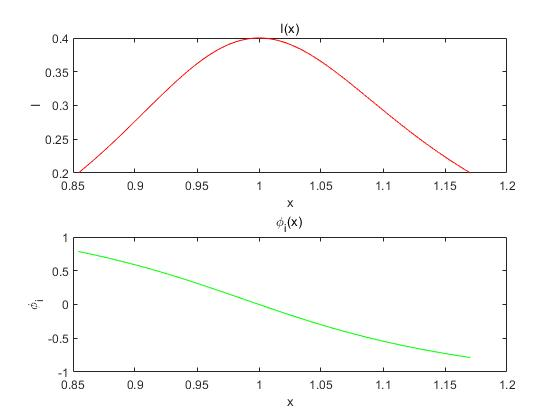
\includegraphics[scale=0.7]{Etude du circuit RLC serie-Resonances//6}
\end{figure}





\begin{lstlisting}[language=matlab]
clc,clear;
E=2;
R=10;
L=100;
C=10;
omega_0=(1/L*C)^(1/2);
Q=omega_0/(R/L);
x_1=-1/(2*Q)+(1+1/(4*Q^2))^(1/2);
x_2=1/(2*Q)+(1+1/(4*Q^2))^(1/2);
x=x_1:0.000001:x_2;
I=E./(R*(1+(Q.*(x-1./x)).^2)*(1/2));
phi_i=-atan(Q.*(x-1./x));
subplot(2,1,1),plot(x,I,'r'),title('I(x)'),xlabel('x'),ylabel('I')
subplot(2,1,2),plot(x,phi_i,'g'),title('{\phi_i}(x)'),xlabel('x'),ylabel('{\phi_i}')
\end{lstlisting}


\section{电荷的谐振}

La réponse en charge, indiquée par la tension  $u_C(t)=\frac{q(t)}{C}$ aux bornes du condensateur
\begin{figure}[H]
	\centering
	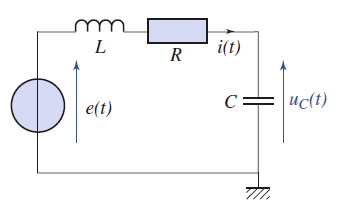
\includegraphics[scale=0.7]{Etude du circuit RLC serie-Resonances//7}
\end{figure}
由于$\underline{q}(t)=\int \underline{i}(t)=\frac{1}{j\omega}\underline{i}(t)$
我们有:$\underline{q}=\frac{1}{j\omega}\underline{I}$

又由于:
$$
\underline{I}=\frac{E/R}{1+jQ(x-1/x)}
$$
我们得到:
$$
\underline{q}=\frac{E/R}{j\omega-\omega Q(x-1/x)}=\frac{E/(R\omega_0)}{jx-xQ(x-1/x)}=\frac{E/(R\omega_0)}{jx-Qx^2+Q}=\frac{E/(R\omega_0Q)}{j\frac{x}{Q}-x^2+1}=\frac{E/(R\omega_0Q)}{1-x^2+j\frac{x}{Q}}
$$

又因为
$$
{\omega_0}^2=\frac{1}{LC}
$$
$$
\frac{\omega_0}{Q}=\frac{R}{L}
$$
所以:
$$
R\omega_0Q=\omega_0^2L=(1/LC)L=1/C
$$
我们得到:
$$
\underline{q}=\frac{CE}{1-x^2+j\frac{x}{Q}}
$$
注意分母这个复数我们在复数章节研究过。
我们直接取振幅:
$$
q=\frac{CE}{\sqrt{(1-x^2)^2+(\frac{x}{Q}})^2}
$$

我们来看看L'amplitude de la charge的一些特殊行为:

Elle est non nulle en $x = 0$ : le condensateur est chargé en régime continu(即之前的暂态) avec
$q_m(0)=CE$. Elle est nulle pour  $x \rightarrow \infty$.

Pour x = 1, nous obtenons $u_C = QE$ : si $Q$ est supérieur à l'unité il y a une {\color{red}surtension}
aux bornes de la capacité.

\begin{figure}[H]
	\centering
	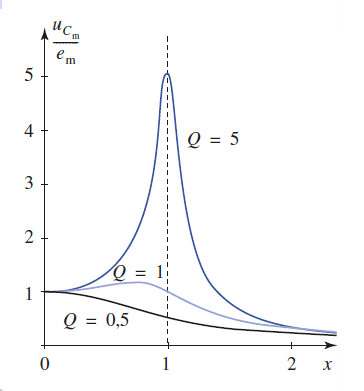
\includegraphics[scale=1]{Etude du circuit RLC serie-Resonances//8}
\end{figure}

下面我们研究谐振的发生条件及情况:

Un éventuel maximum de $q$ correspond au minimum de :
$$
D(x)=(1-x^2)^2+(\frac{x}{Q})^2
$$
La dérivée
 $$D'(x)=2(1-x^2)(-2x)+2x/Q^2=4x(x^2-1+1/2Q^2)=4x(x^2-(1-1/2Q^2))$$
  s'annule en $x = 0$, et en $x=\sqrt{1-1/2Q^2}$,cette racine n'existe que si $Q>1/\sqrt{2}$.Une résonance en tension est donc observable si cette condition est vérifiée.

La pulsation de résonance, lorsqu‘elle existe correspond à :
$$
\omega_r=\omega_0\sqrt{1-1/2Q^2}
$$
Dans ce cas, la résonance est obtenue pour une pulsation $\omega_r$ inférieure
à $\omega_0$ . Si $Q\gg1$, $\omega_r$ est voisin de $\omega_0$ .

下面来看一下bande passante.首先我们要看一下振幅$q$的最大值:
$$
\begin{aligned}
q(\sqrt{1-1/2Q^2})&=\frac{CE}{\sqrt{(1-(\sqrt{1-1/2Q^2})^2)+(\sqrt{1-1/2Q^2})^2/Q^2}}\\
&=\frac{CE}{\sqrt{(1-(1-1/2Q^2))^2+(1-1/2Q^2)/Q^2}}\\
&=\frac{CE}{\sqrt{1/4Q^4+1/Q^2-1/2Q^4}}\\
&=\frac{CE}{\sqrt{1/Q^2-1/4Q^4}}\\
&=\frac{CEQ}{\sqrt{1-1/4Q^2}}
\end{aligned}
$$
我们要解出方程:
$$
\frac{CEQ}{\sqrt{2-2/4Q^2}}=\frac{CE}{\sqrt{(1-x^2)^2+(\frac{x}{Q}})^2}
$$
$$
(1-x^2)^2+(\frac{x}{Q})^2=2/Q^2-1/2Q^4
$$
这个方程非常复杂,所以我们需要求特殊情况下的近似解。

我们有现象:在非常欠阻尼($Q\gg 1$)振子的情况下,电荷谐振非常明显以至于我们可以认为$x_r,1/2\approx 1$,这时我们有:
$$-1/2Q^4\approx0$$
$$x^2\approx1$$
$$
(1-x^2)^2=(1-x)^2(1+x)^2\approx(1-x)^2(1+1)^2=4(1-x)^2
.$$

所以
$$
\begin{aligned}
4(1-x)^2=2/Q^2-1/Q^2=1/Q^2\\
1-x=\pm1/2Q\\
x=1\mp1/2Q\\
\Delta x=1/Q
\end{aligned}
$$
所以谐振锐度为$1/\Delta x=Q$.\textbf{在非常欠阻尼的情况下,我们有: $Q$越大,谐振锐度越大}。

最后我们看看Déphasage:

Sachant que $\underline{q}=qe^{j\varphi}=\underline{I}/j\omega=\frac{Ie^{j(\phi-\frac{\pi}{2})}}{\omega}$
nous en déduisons que la
phase de la charge du condensateur vaut :
$$
\varphi=\phi-\frac{\pi}{2}=-\arctan{Q(x-1/x)}-\frac{\pi}{2}
$$
注意$\underline{q}$的dephasage是间接求得的,不是它原本的相角表达式,原本是一个分段函数且$\arctan$中的量也与间接求出的不同。

Cette phase est nulle à basse fréquence ($x\ll1$), et décroît jusqu’à $–\pi$ à haute
fréquence ($x\gg1$). Lorsque le circuit est excité à sa pulsation propre, la charge du condensateur est en phase avec la tension excitatrice.La rotation de phase au voisinage de $x=1$ est d’autant plus rapide que le facteur de qualité Q est élevé.
de $Q$

\begin{figure}[H]
	\centering
	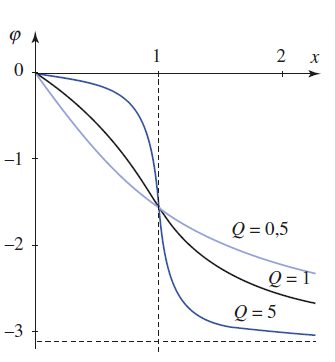
\includegraphics[scale=0.8]{Etude du circuit RLC serie-Resonances//9}
\end{figure}
\section{Circuits linéaires en régime sinusoïdal}
\subsection{Régime forcé d’un circuit linéaire}
\textbf{L'étude effectuée pour le circuit (R,L,C) série peut être généralisée aux
	réseaux linéaires}, lorsqu'ils sont soumis à une excitation sinusoïdale : la
réponse du circuit à une excitation sinusoïdale est la superposition de la
réponse permanente sinusoïdale (qui ne dépend pas des conditions initiales) et
d'un régime transitoire (déterminé par les conditions initiales).
Nous supposerons que le régime libre du circuit est caractérisé par un régime
transitoire qui tend vers zéro au cours du temps : le circuit est supposé stable,
suffisamment amorti.
\subsection{Étude du régime sinusoïdal forcé}
Chaque branche du circuit est régie par une équation d'évolution qui est une
équation différentielle linéaire à coefficients constants. Pour étudier le régime
sinusoïdal permanent établi, nous savons qu'il est très commode d'utiliser la
notation complexe. L'équation différentielle se ramène alors à une relation
entre amplitudes complexes où interviennent des polynômes de la variable ($j\omega$).
Par exemple, pour un circuit dont l'évolution est régie par l'équation:
$$
D_2\frac{\mathrm{d^2}s(t)}{\mathrm{d}t^2}+D_1\frac{\mathrm{d}s(t)}{\mathrm{d}t}+D_0s(t)=N_2\frac{\mathrm{d^2}e(t)}{\mathrm{d}t^2}+N_1\frac{\mathrm{d}e(t)}{\mathrm{d}t}+N_0e(t)
$$
liant sa réponse $s(t)$ à l'excitation $e(t)$, nous obtenons immédiatement le rapport
des amplitudes complexes de l'excitation et de la réponse sous la forme
d'un rapport de deux polynômes de la variable ($j\omega$).
$$
\frac{\underline{s}}{\underline{e}}=\frac{-\omega^2N_2+j\omega N_1+N_0}{-\omega^2D_2+j\omega D_1+D_0}=\frac{N(j\omega)}{D(j\omega)}
$$

\begin{figure}[H]
	\centering
	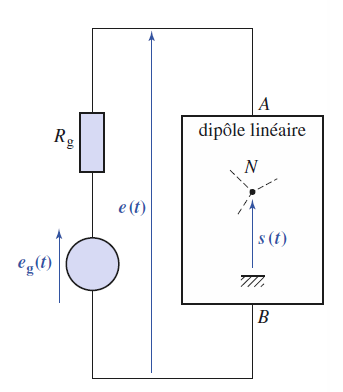
\includegraphics[scale=1]{Etude du circuit RLC serie-Resonances//10}
\end{figure}
\chapter{Analyse de Fourier d'un signal périodique}
\begin{framed}{\textbf{定理}}
Tout signal physique périodique est décomposable en une somme de signaux sinusoïdaux.
D'un point de vue physique, cela veut dire que, connaissant {\color{red}la décomposition du signal d'entrée} pour un système linéaire dont {\color{red}la fonction de transfert} est aussi connue, alors on peut donner {\color{red}le signal de sortie} en faisant les calculs composante par composante(c'est-à-dire un principe de superposition "harmonique",fréquence par fréquence)
\end{framed}
\textbf{Coefficients de Fourier}

Les coefficients de Fourier interviennent dans l'expression de la décomposition en série de Fourier d'un signal en pondérant l'amplitude de chaque composante;ces coefficients \textbf{dépendent de la fonction définissant le signal}.

Soit $f(t)$ le signal entrée, de période $T$, on a alors, en notant $\omega=\frac{2\pi}{T}$,la décomposition en série de Fourier de $f(t)$ qui est unique ,est donné par 
$$
\boxed{f(t)=a_0+\sum_{n=1}^{\infty}a_n\cos(n\omega t)+b_n\sin(n\omega t)}
$$
avec la définition suivante pour les coefficients de Fourier $a_n$ et $b_n$,on note $t_0$ un instant quelconque pris comme origine
$$
\boxed{a_0=\frac{1}{T}\int_{t_0}^{t_0+T}f(t)dt}
$$  
$$
\boxed{a_n=\frac{2}{T}\int_{t_0}^{t_0+T}f(t)cos(n\omega t)dt}
$$
$$
\boxed{b_n=\frac{2}{T}\int_{t_0}^{t_0+T}f(t)sin(n\omega t)dt}
$$
On peut aussi écrire $f(t)$ sous la forme suivante:
$$
\boxed{f(t)=c_0+\sum_{n=1}^{\infty}c_n\cos(n\omega t+\phi_{n}}
$$
avec $c_0=a_0$,$c_n=\sqrt{a_n^2+b_n^2}$ et $\tan(\phi_{n})=-\frac{b_n}{a_n}$.

$c_0$ est la composante continue ou la valeur moyenne de $f$,$c_n$ est l'amplitude de l'harmonique de rang $n$ et $\phi_{n}$ le déphasage(ou phase à l'origine) de l'harmonique de rang $n$.

\textbf{Égalité de Parseval}

$$
\boxed{\left \langle f^2(t) \right \rangle _{T}=\frac{1}{T}\int_{0}^{T}f^2(t)dt=c_0^2+\sum_{n=1}^{\infty}\frac{c_n^2}{2}}
$$



\textbf{Spectre de fréquences}

Le spectre de la fonction $f$ est obtenu en portant en ordonnée l'amplitude des harmoniques $(c_n)$ et abscisse les pulsations(ou fréquences) correspondantes.On a alors \textbf{le diagramme en bâtons} suivant:
\begin{figure}[H]
	\centering
	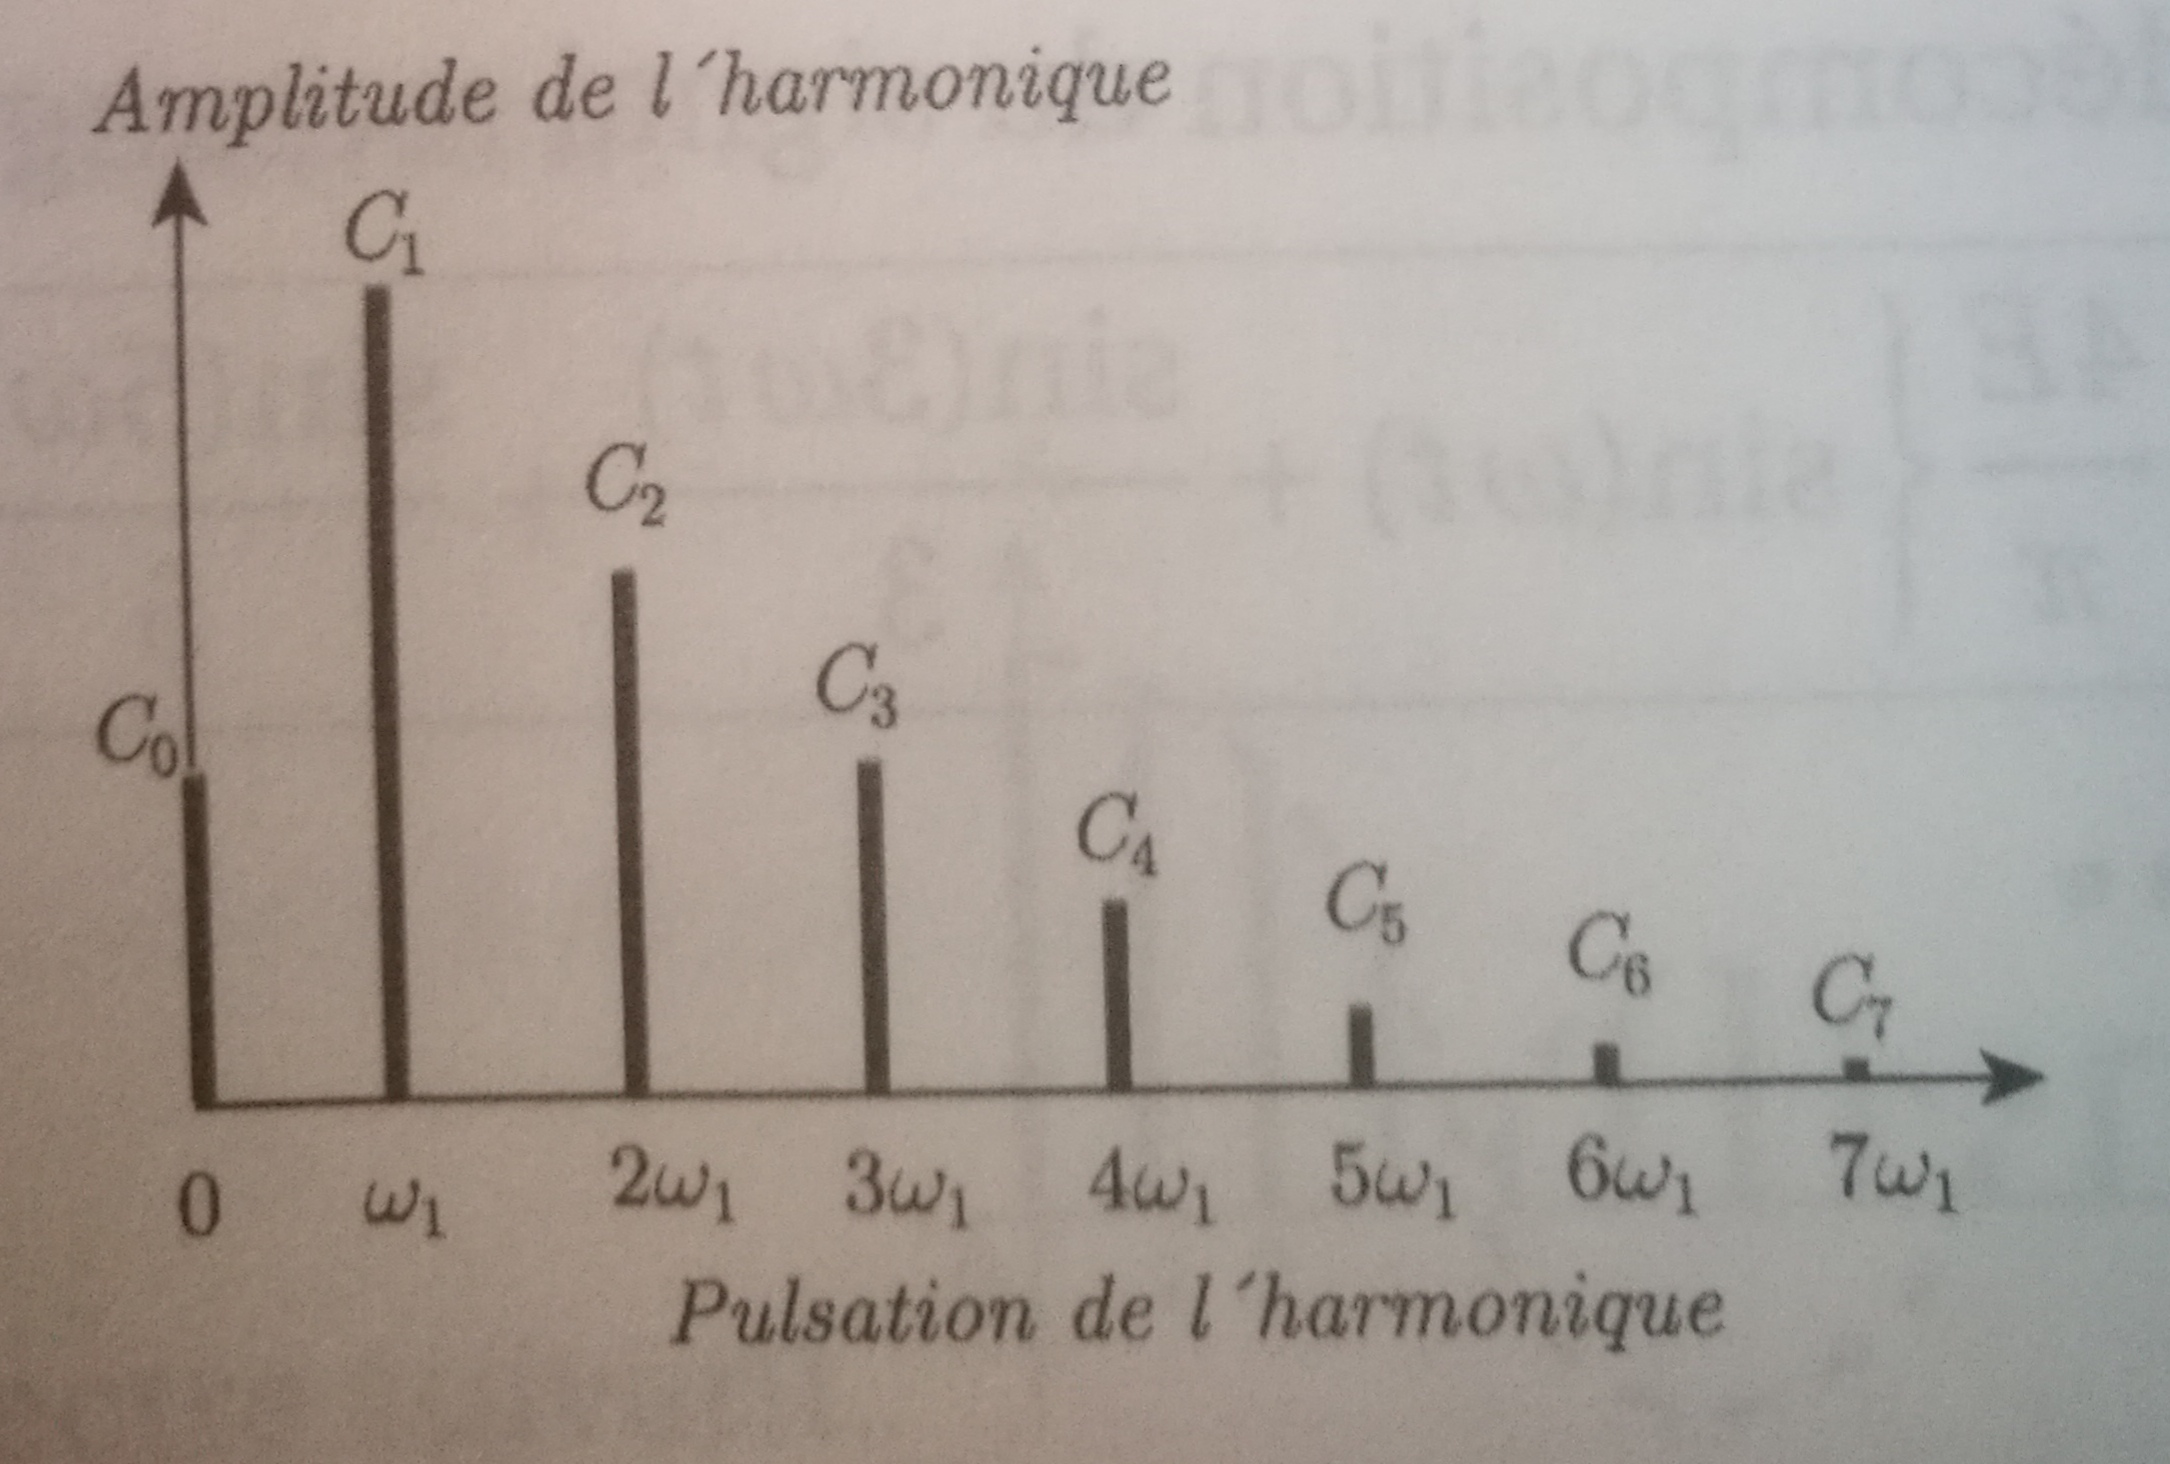
\includegraphics[scale=0.1]{Analyse de Fourier d'un signal periodique//1}
\end{figure}

\textbf{Signal carré}

On considère un signal créneau impaire de période $T$ variant entre $-E$ et $E$.On a alors:
$$
a_0=a_n=0
$$
$$
\begin{aligned}
b_n&=\frac{2}{T}\int_{-T/2}^{T/2}f(t)sin(n\omega t)dt\\
&=\frac{2}{T}\int_{-T/2}^{0}(-E)sin(n\omega t)dt+\frac{2}{T}\int_{0}^{T/2}Esin(n\omega t)dt\\
&=\frac{2E}{T}\left \{ \left(\frac{cos(n\omega t)}{n\omega}\right)_{-T/2}^0+\left(-\frac{cos(n\omega t)}{n\omega}\right)_0^{T/2} \right \} \\
&=\frac{2E}{n\pi}(1-cos(n\pi))
\end{aligned}
$$
On a donc obtenu la décomposition du signal rectangulaire qui est 
$$
\boxed{f(t)=\frac{4E}{\pi}\left \{ sin(\omega t) +\frac{sin(3\omega t)}{3}+\frac{sin(5\omega t)}{5}+...\right \} }
$$
\begin{figure}[H]
	\centering
	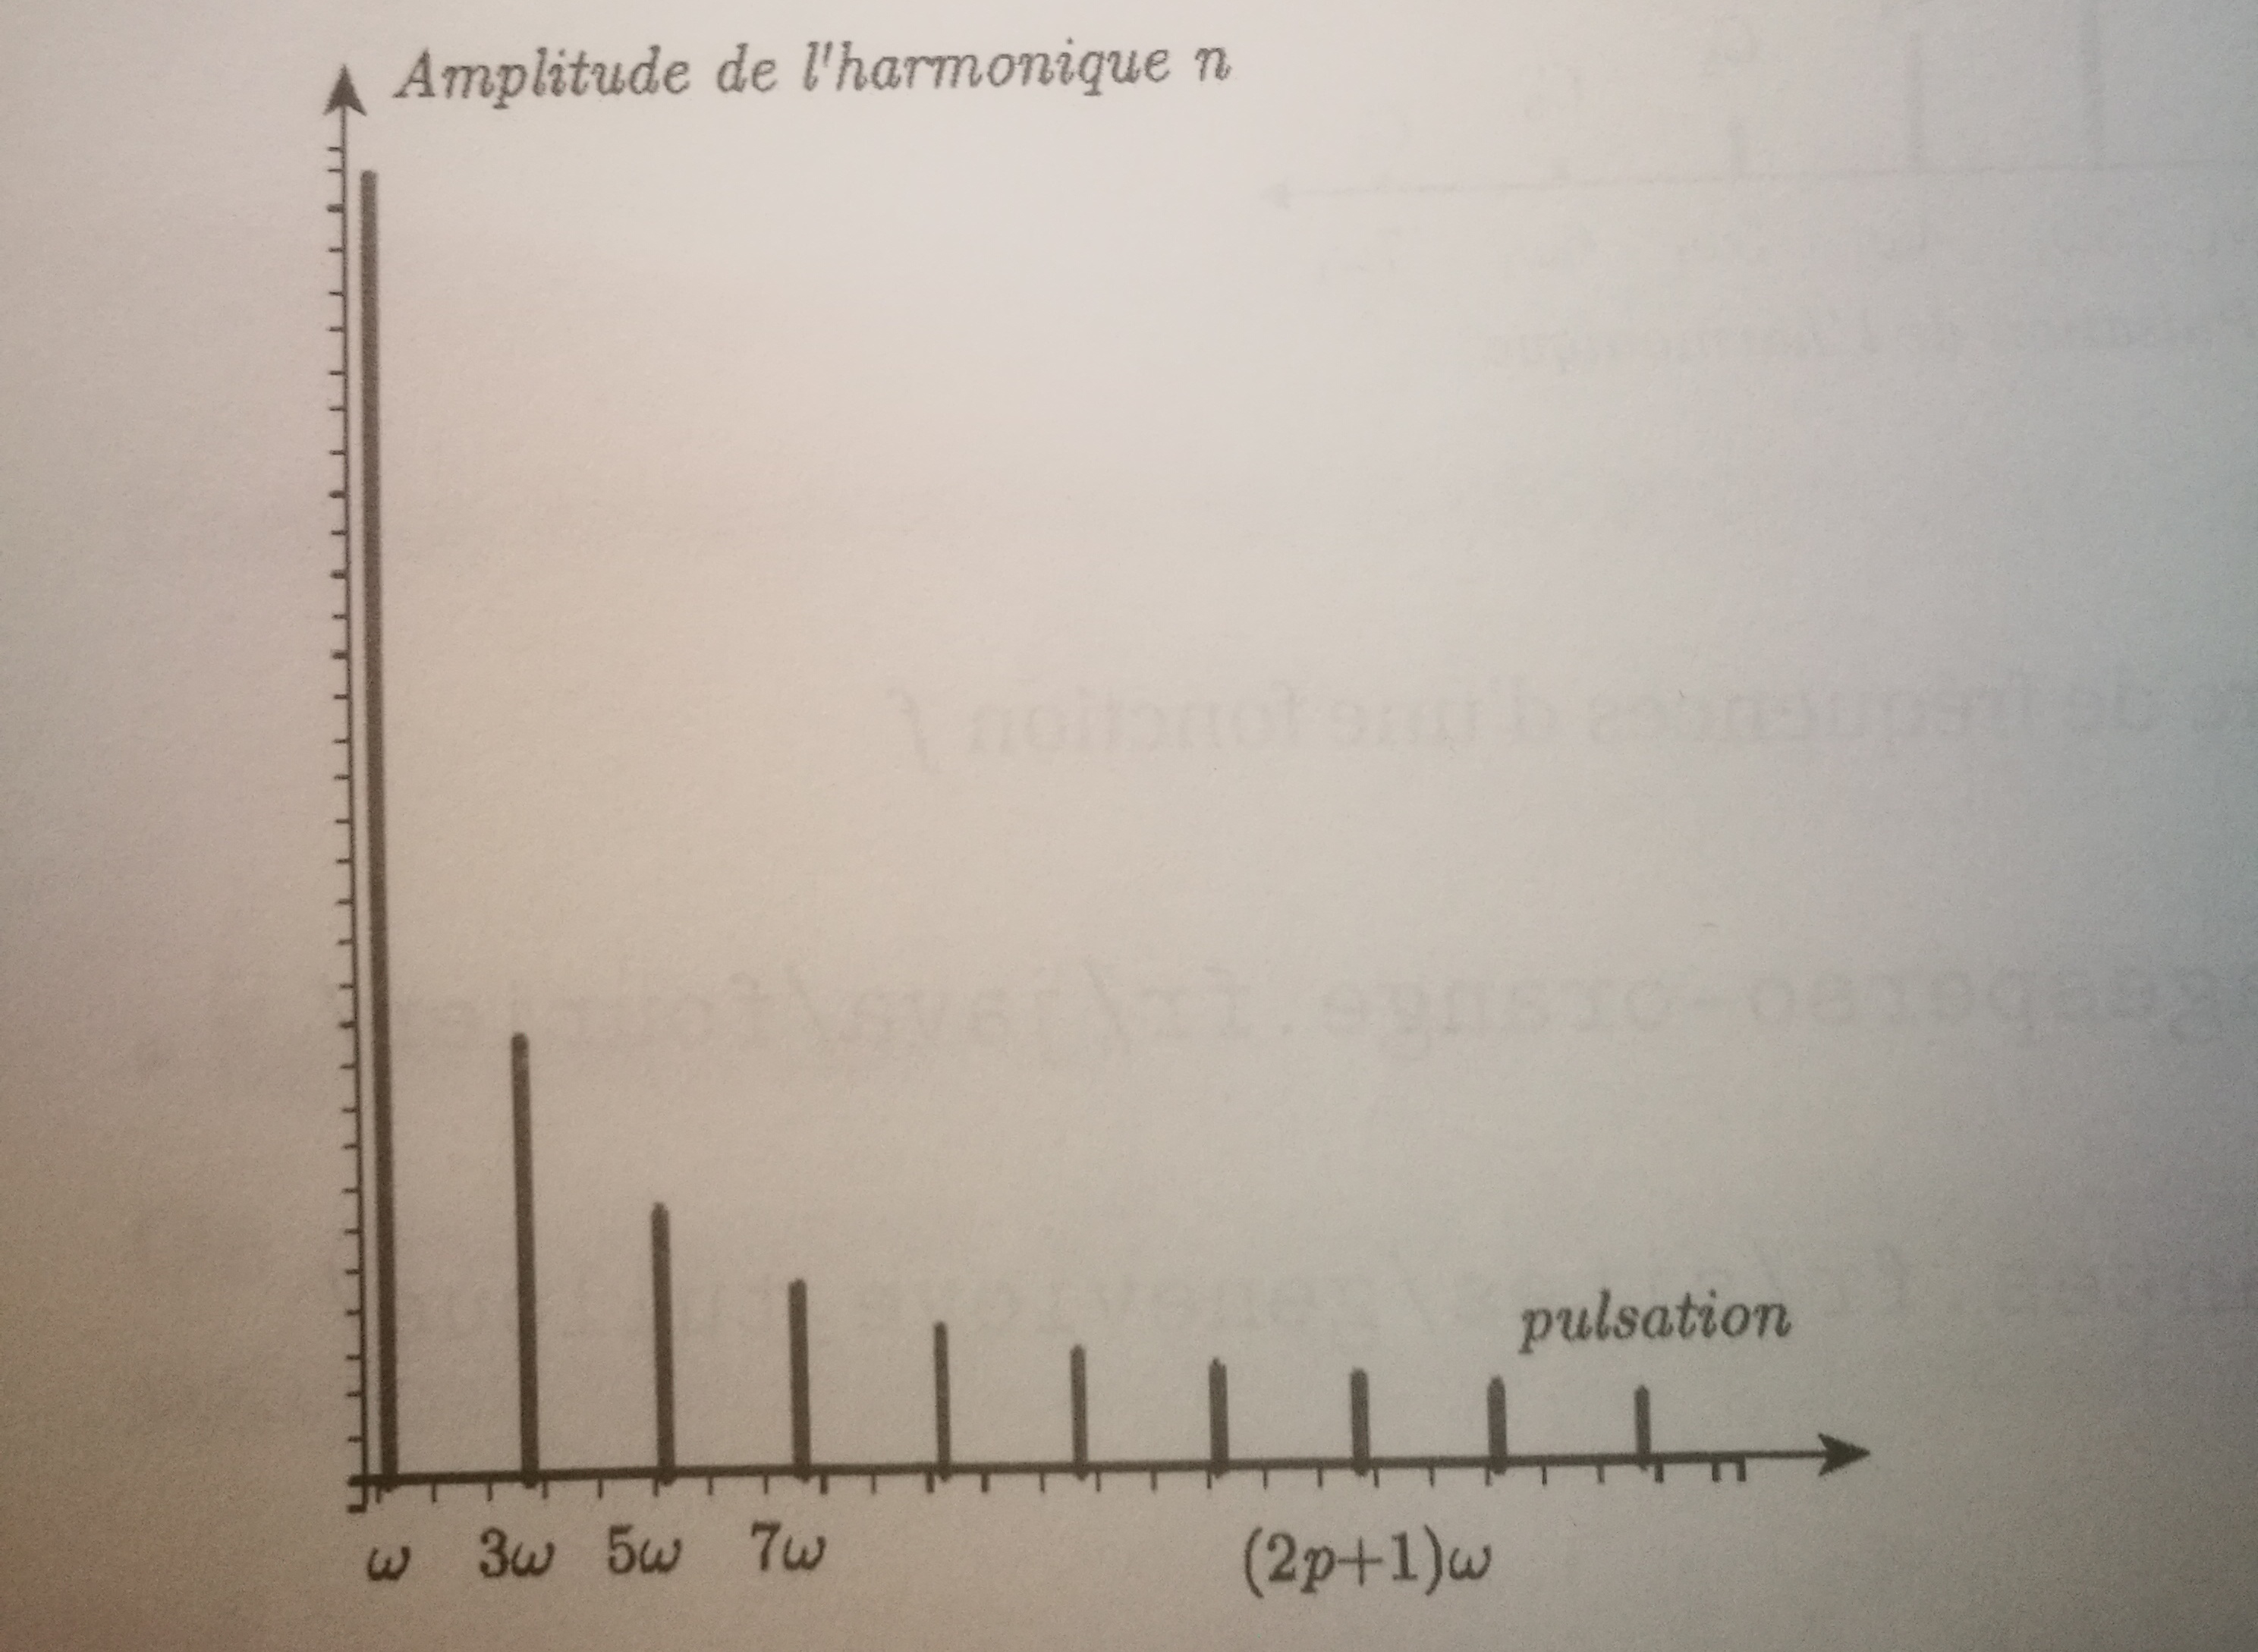
\includegraphics[scale=0.1]{Analyse de Fourier d'un signal periodique//2}
\end{figure}


\chapter{Filtrage}
\section{Fonction de transfert}
\begin{framed}{\textbf{研究对象}}
On considère un quadripôle(c'est-à-dire un dipôle avec 2 bornes d'entrée et 2 bornes de sortie) soumis à une tension sinusoïdal $v_e(t)=v_e cos(\omega t)$ de pulsation $\omega$ variable.On cherche donc à connaître $v_s(t)$.
\end{framed}

\begin{framed}{\textbf{框架}}
	On ne considère que des quadripôles en sortie ouverte soit $i_s=0$, ce qui est réalisé si on ne branche rien en sortie ou si on met un dipôle de charge d'impédance d'entrée infinie.
	
	On étudie la réponse du système en régime permanent.Pour un circuit linéaire, on s'intéresse donc à la réponse du système à la même fréquence que celle imposée par le générateur.
\end{framed}

\begin{figure}[H]
	\centering
	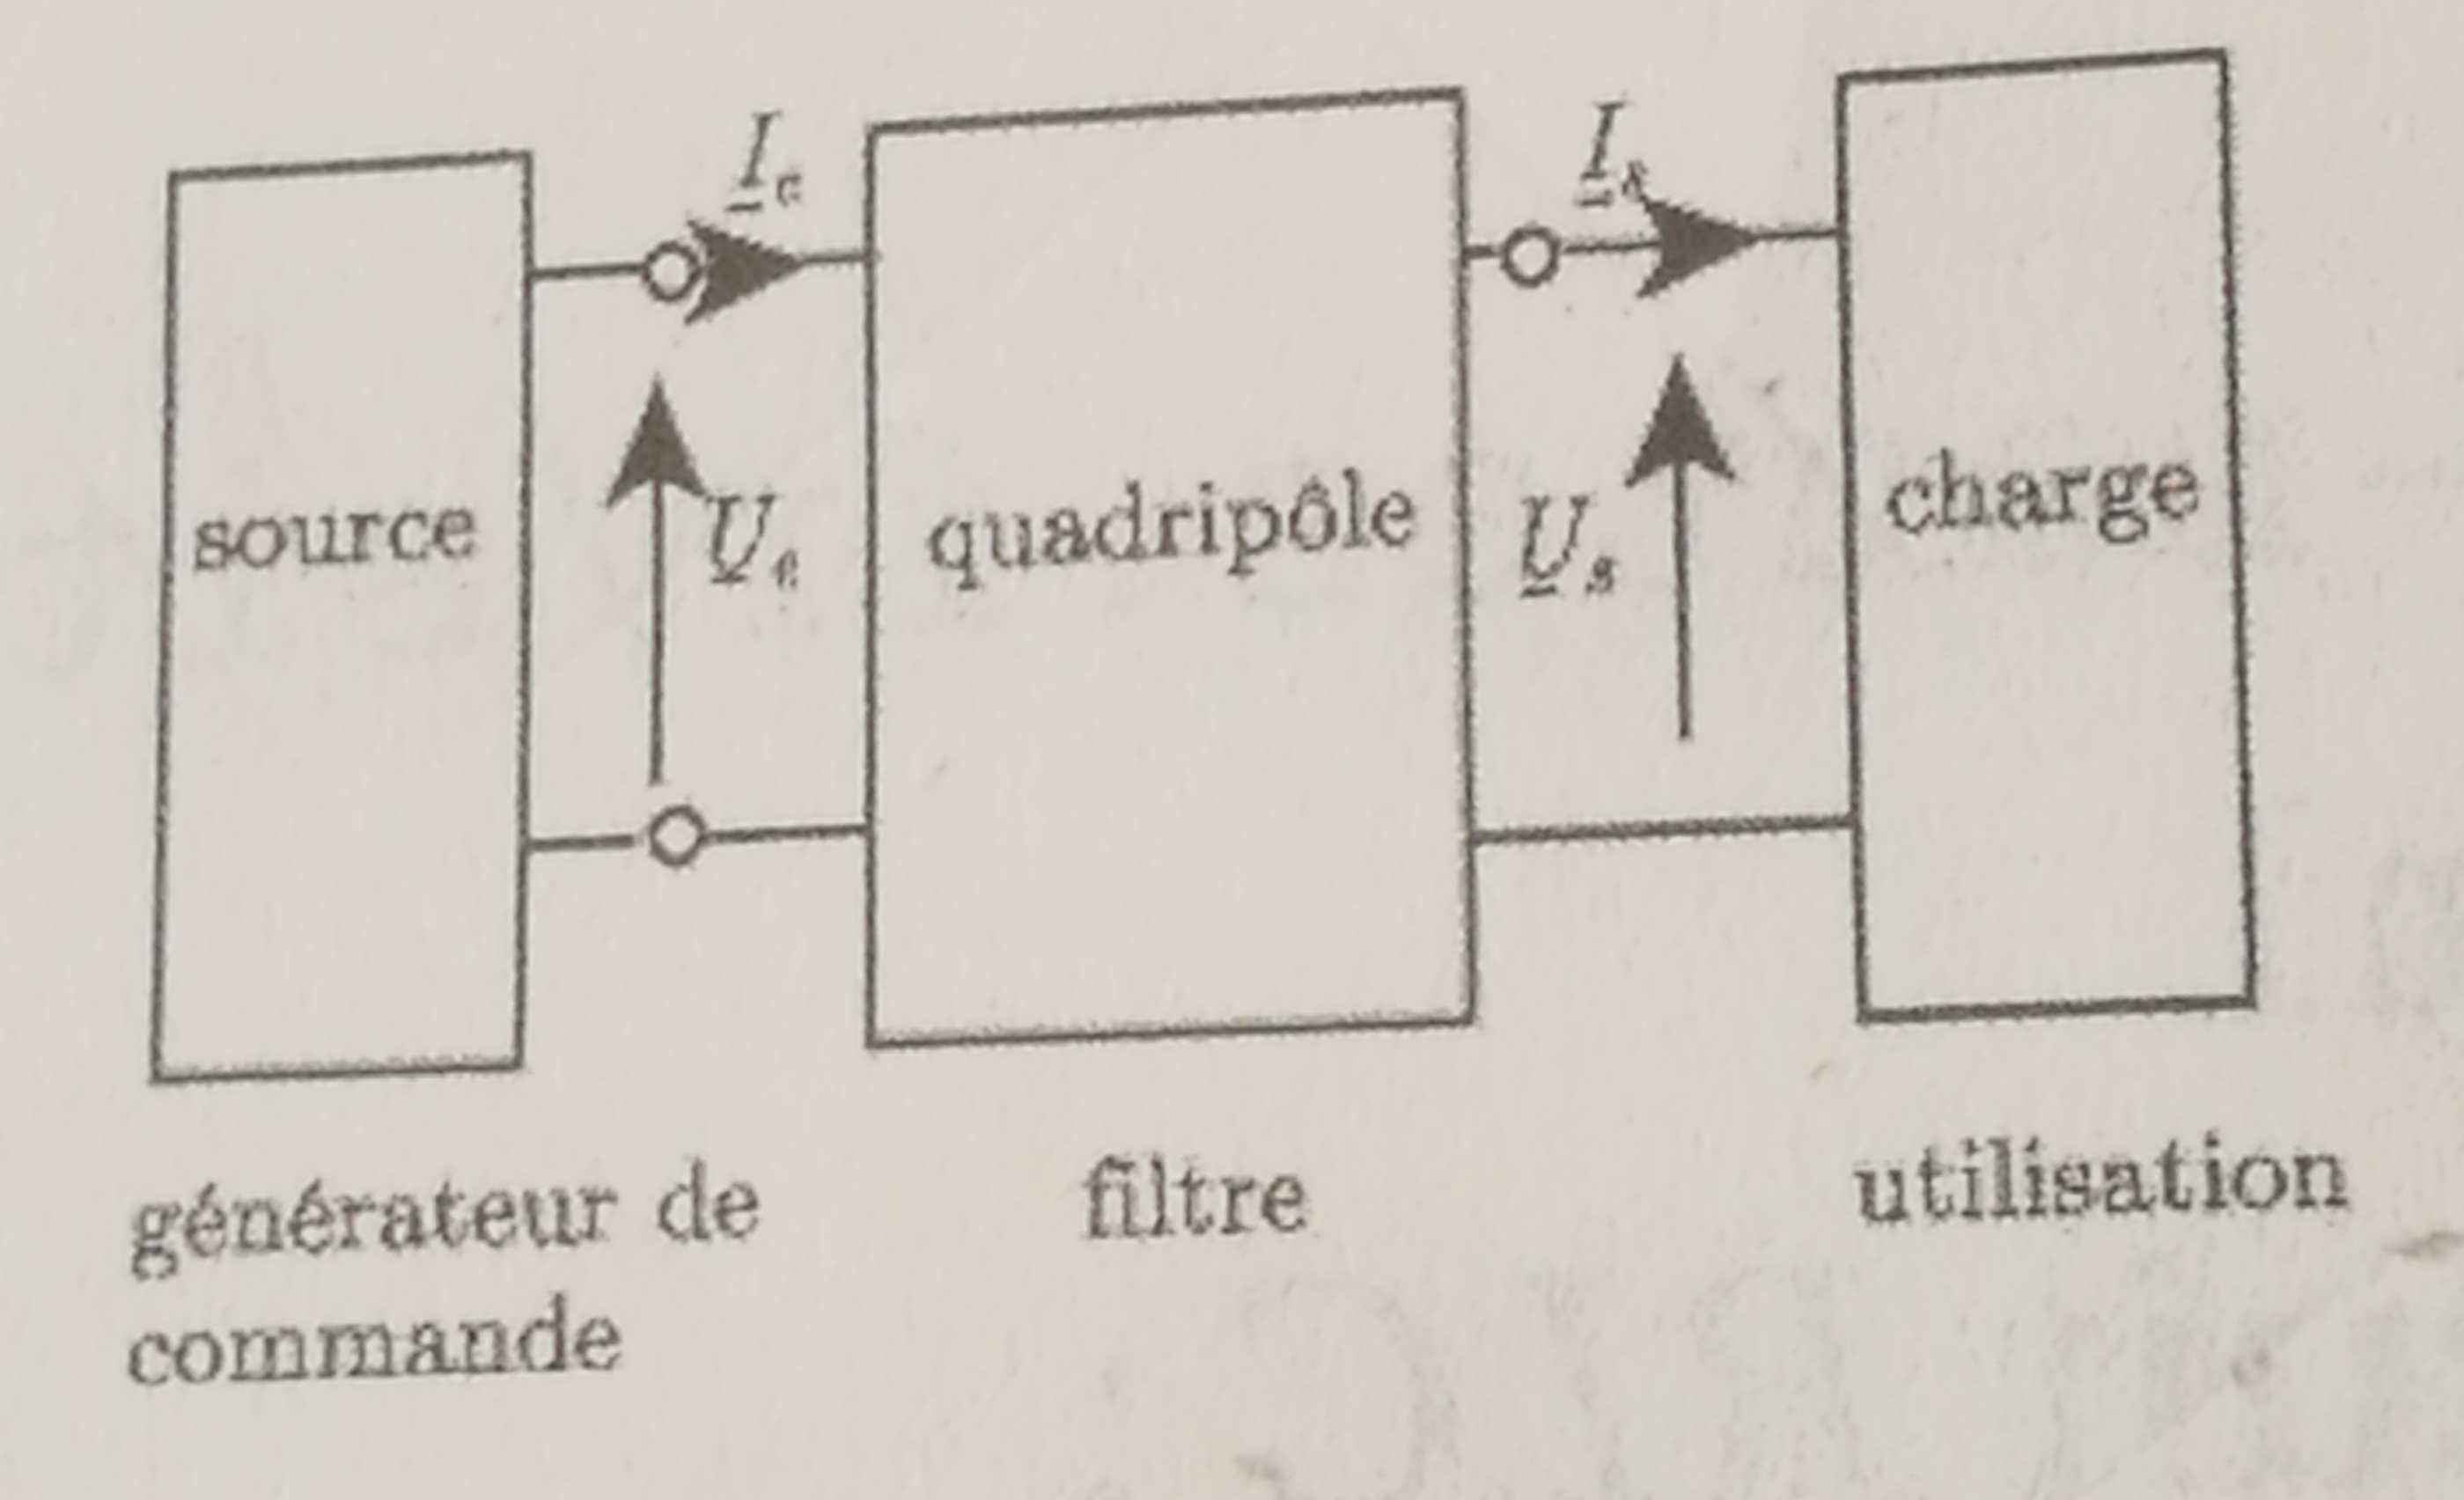
\includegraphics[scale=0.08]{Filtrage//1}
\end{figure}


\begin{framed}{\textbf{定义}}
On définit la fonction de transfert $H$ par 
$$
\underline{H}(j\omega)=\frac{\underline{v_s}}{\underline{v_e}}=G(\omega)e^{j\phi(\omega)}
$$ 	
avec $G(\omega)$ le gain en tension et $\phi(\omega)$ l'avance de phase de $v_s$ par rapport à $v_e$

On définie aussi {\color{red}le gain en décibels}
$$
G_{dB}=20\log G
$$	
\end{framed}

\begin{framed}
	\begin{prp}
	$v_s(t)=\left| \underline{H}\right|\times v_e \times \cos (\omega t + \phi(\underline{H}))$
	\end{prp}
\end{framed}


\section{Diagramme de Bode}
\begin{framed}{\textbf{框架}}
Un quadripôle ou un filtre a une réponse en amplitude et en phase qui dépend de la fréquence!
\end{framed}
\begin{framed}{\textbf{定义}}
On définit le diagramme de Bode d'un filtre comme la donné de 
$$
G_{dB}=f(\log\omega)\quad \text{et} \quad\phi=g(\log\omega)
$$

On appelle {\color{red}décade} un intervalle de fréquence qui correspond à un rapport 10 entre les fréquence extrêmes.(区间端点频率之比为10)
\end{framed}
\begin{framed}
\begin{prp}{\textbf{Bande passante à -3 dB}}
C'est l'intervalle des fréquences(ou de pulsations) tel que: 	
	$$G_{dB}\ge G_{dB,max}-3dB$$
	
$\log2=0.3$
\end{prp}
\end{framed}
\begin{framed}{\textbf{定理}}
	Un filtre linéaire est un quadripôle linéaire qui atténue (gain de la fonction de transfert $G<1$) certaines fréquences et en laisse passer d'autres, parfois en les amplifiant.   
\end{framed}
\begin{framed}{\textbf{定义}}
	Un filtre est dit passif quand il ne contient que des dipôles passifs(résistance, bobine ,condensateur...) soit aucune source d'énergie extérieur.Ces filtres sont caractérisés par un gain faible.
\end{framed}
\section{Filtres du premier ordre}
\begin{framed}{\textbf{定义}}
Filtres du premier ordre est un système dont la fonction de transfert présente {\color{red}un dénominateur du premier ordre en $j\omega$} ou $jx$ avec la pulsation réduite.
\end{framed}

\subsection{Filtre passe-bas}
\begin{framed}{\textbf{框架}}
On s'intéresse au circuit $LR$ suivant.La tension de sortie est la tension $u_r$ aux bornes de la résistance $R$.
\end{framed}
\begin{figure}[H]
	\centering
	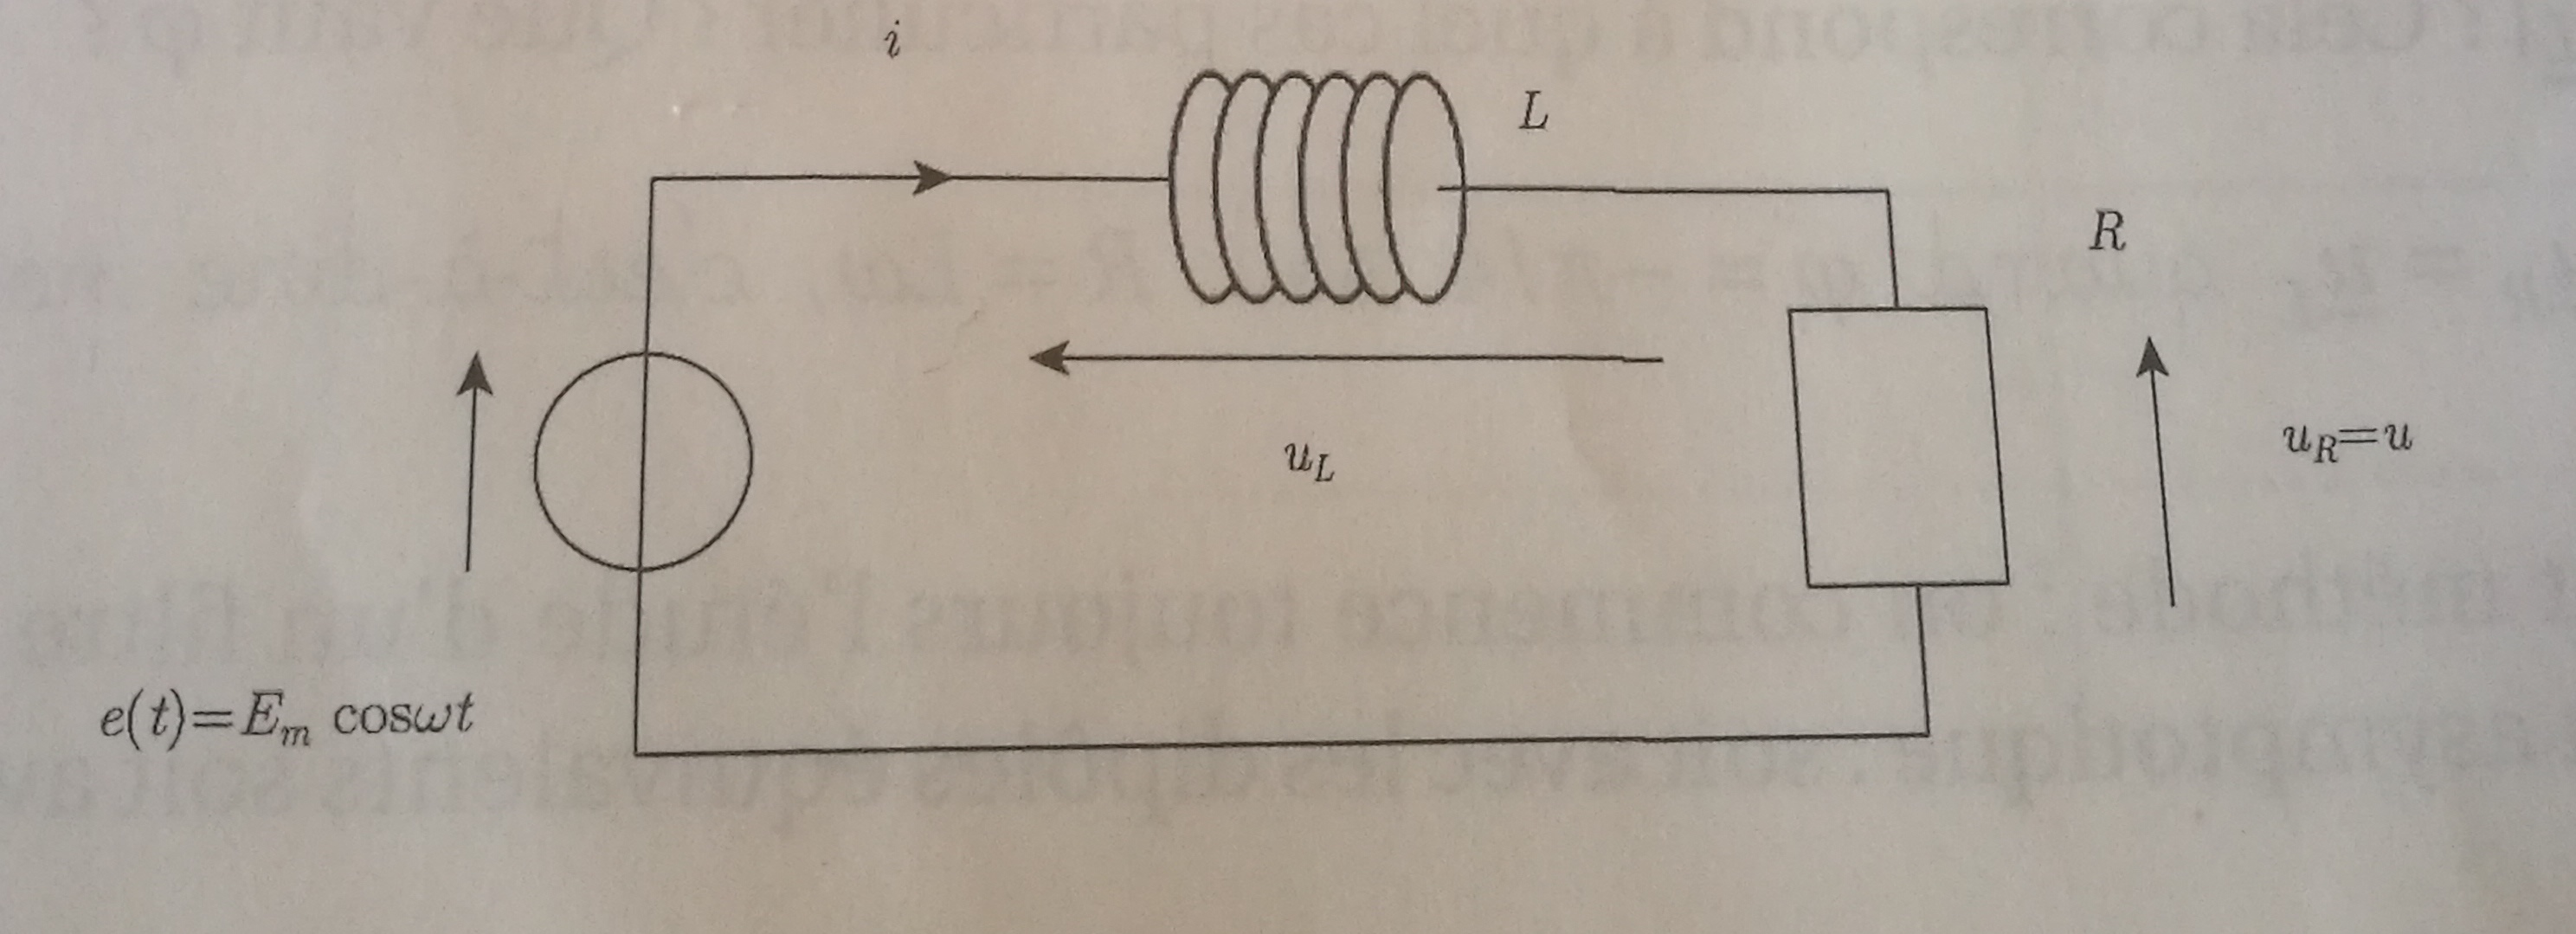
\includegraphics[scale=0.13]{Filtrage//2}
\end{figure}
我们从\textbf{comportement asymptomatique}开始研究,这是为了首先确定la nature du filtre.我们画出在低频和高频时的等效电路图:
\begin{figure}[H]
	\centering
	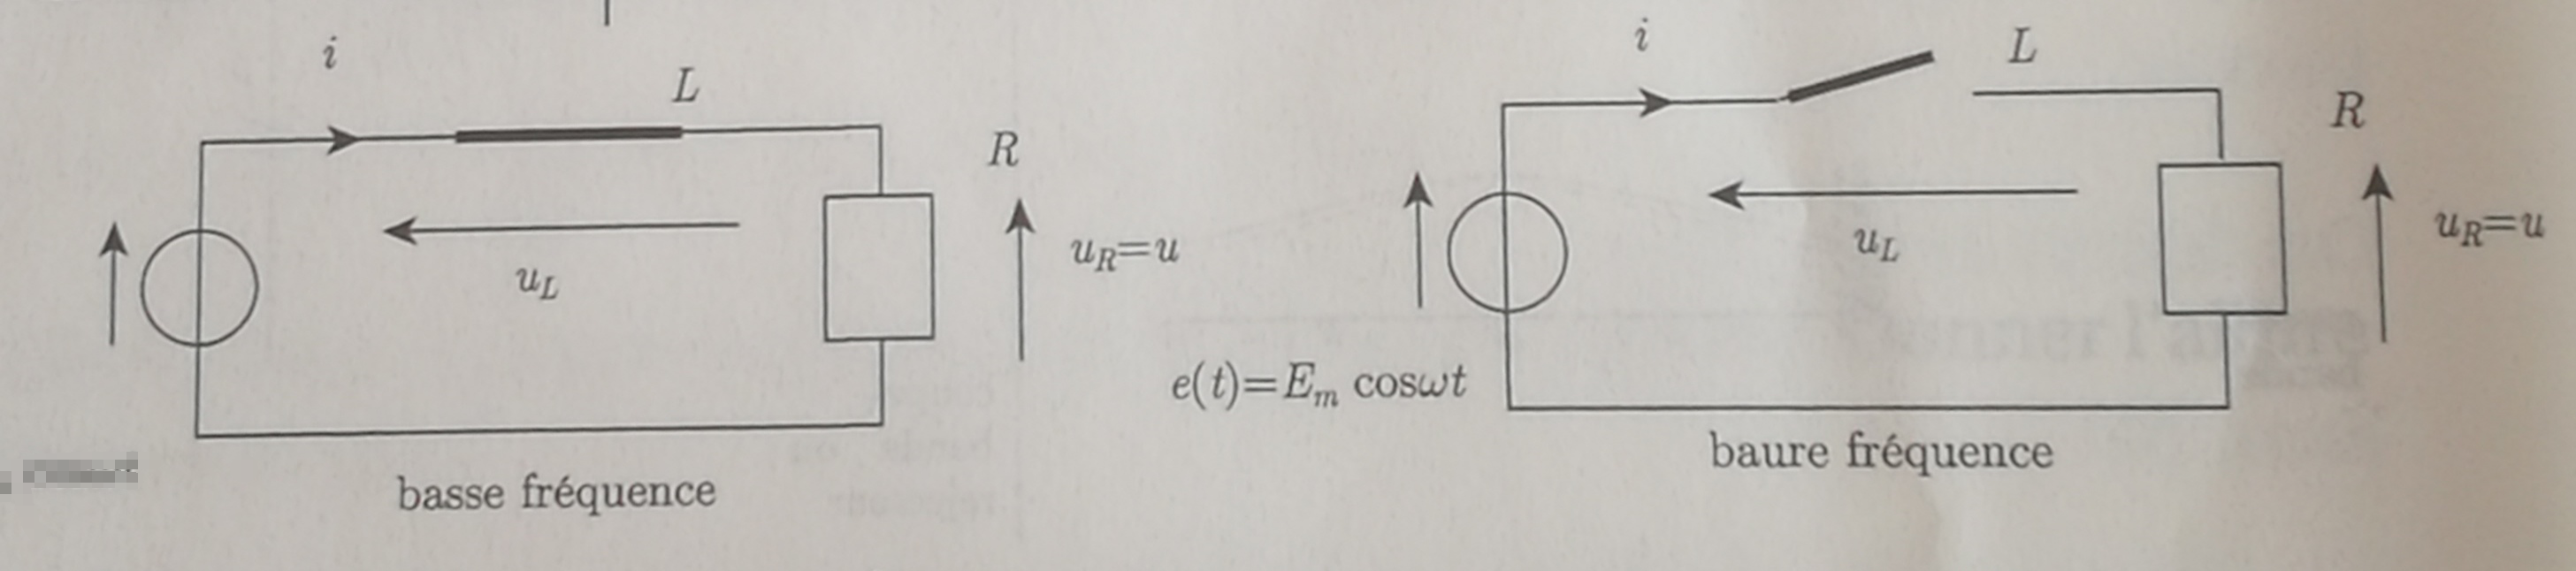
\includegraphics[scale=0.15]{Filtrage//3}
\end{figure}
可以看到低频的信号可以输出,而高频的信号输出为0从而失去影响,从而该电路的确是一个“低通”滤波器。

然后我们开始传递函数的研究.

首先我们确定特征角频率:
$$
Ri(t)+L\frac{\mathrm{d}i(t)}{\mathrm{d}t}=e(t)
$$
$$
\frac{\mathrm{d}i(t)}{\mathrm{d}t}+\frac{R}{L}i(t)=e(t)/L
$$
又
$$
\frac{\mathrm{d}i(t)}{\mathrm{d}t}+\omega_0i(t)=e(t)/L
$$
对应的$\omega_0=\frac{R}{L}$
\begin{framed}
	$$
	\underline{H}=\frac{\underline{Z}_R}{\underline{Z}_R+\underline{Z}_L}=\frac{R}{R+jL\omega}=\frac{1}{1+j\omega/\omega_0}=\frac{1}{1+jx}
	$$
\end{framed}

接着我们试作出le diagramme de Bode.

首先写出增益和相位差的函数:
$$
G(x)=\frac{1}{\sqrt{1+x^2}}
$$
$$
\phi(x)=-\arctan(x)
$$
然后我们要做三件工作:
\begin{itemize}
	\item 找出截断角频率对应的$x_c$:由定义,我们有$G(x_c)=1/\sqrt{2}$ ,soit$x_c=1$
	\item 
	由于$\log$的单调递增性,由复合单调性的符号规则,我们可以直接从$G(x)$的趋势得出$G_{dB}(\log x)$的趋势,从$\phi(x)$的趋势得出$\phi(\log x)$的趋势。这里两个的趋势都是单调递减的。
	\item 然后我们研究极限渐进情况下的$G_{dB}(\log(x))$和$\phi(\log x)$,由于换了变量并不改变实质的内容我们研究的时候可以从原来的函数$G_{dB}(x)=-10\log(1+x^2)$和$\phi(x)$出发,最后若得到一个等价的函数(若函数趋于无穷则有这个需要)再换回$\log x$作为变量.这里我们有:
	$$
	\lim\limits_{x\to 0}G_{dB}(x)=0
	$$
	$$
	G_{dB}\underset{x\to\infty}{\sim}-20\log(x)
	$$
	$$
	\lim\limits_{x\to0}\phi(x)=0
	$$
	$$
	\lim\limits_{x\to \infty}\phi(x)=-\frac{\pi}{2}
	$$
	
	从而换回变量$\log(x)$(注意此时的趋向与变量为$x$时的趋向表述不一样了)后,$G_{dB}(\log x)$在负无穷处(对应$x\to0$)有一条水平渐近线,在正无穷处有一条过原点的斜率为-20dB/décade的渐近(直)线.
\end{itemize}

\begin{figure}[H]
	\centering
	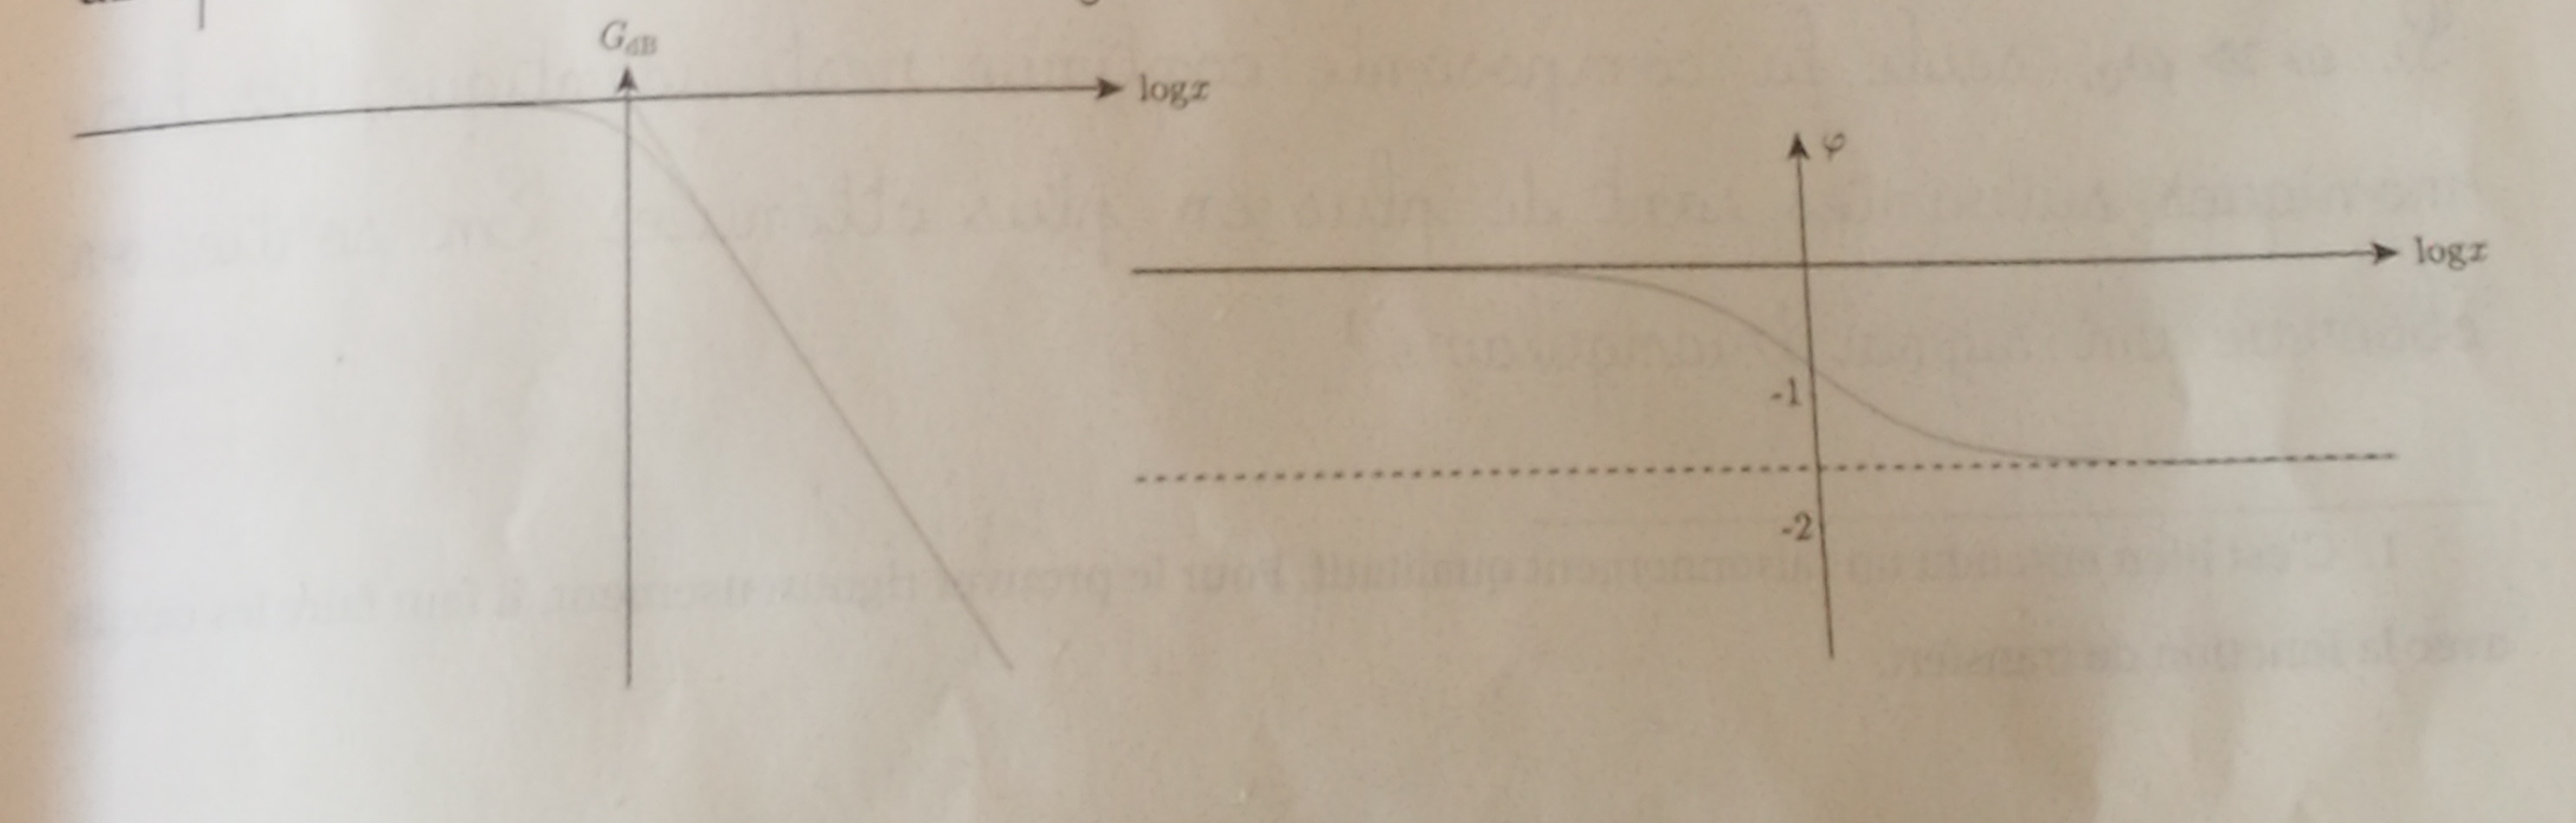
\includegraphics[scale=0.16]{Filtrage//4}
\end{figure}

最后我们看看低通滤波器对高频的信号的处理特性(低频的信号通“过”了,滤波器所起的作用看不出什么特点)。其实对高频段的信号,滤波器表现得像是一个“赝积分器”(pseudo-intégrateur).
\begin{framed}{\textbf{定理}}
	对$x\gg1$的信号$v_s(t)$,我们可以写出经过传递函数联系的它与$v_s(t)$之间的关系式,此时传递函数近似为$\underline{H}=\frac{1}{jx}$,对应的$\underline{v}_s=\omega_0\frac{\underline{v}_e}{j\omega}$=$\omega_0$$\int\underline{v}_e(t)dt$,从而$v_s=\omega_0\int v_e(t)dt$.
\end{framed}

\section{Filtres du deuxième ordre}

\begin{framed}{\textbf{定义}}
	Filtre du deuxième ordre est un système dont la fonction de transfert présente un dénominateur du second ordre en $j\omega$ et {\color{red} un numérateur d'ordre au plus 2}
\end{framed}

\subsection{Filtre passe-haute}
\begin{framed}{\textbf{框架}}
On s'intéresse dans le circuit suivant à la réponse en tension aux bornes de la bobine.
\end{framed}
\begin{figure}[H]
	\centering
	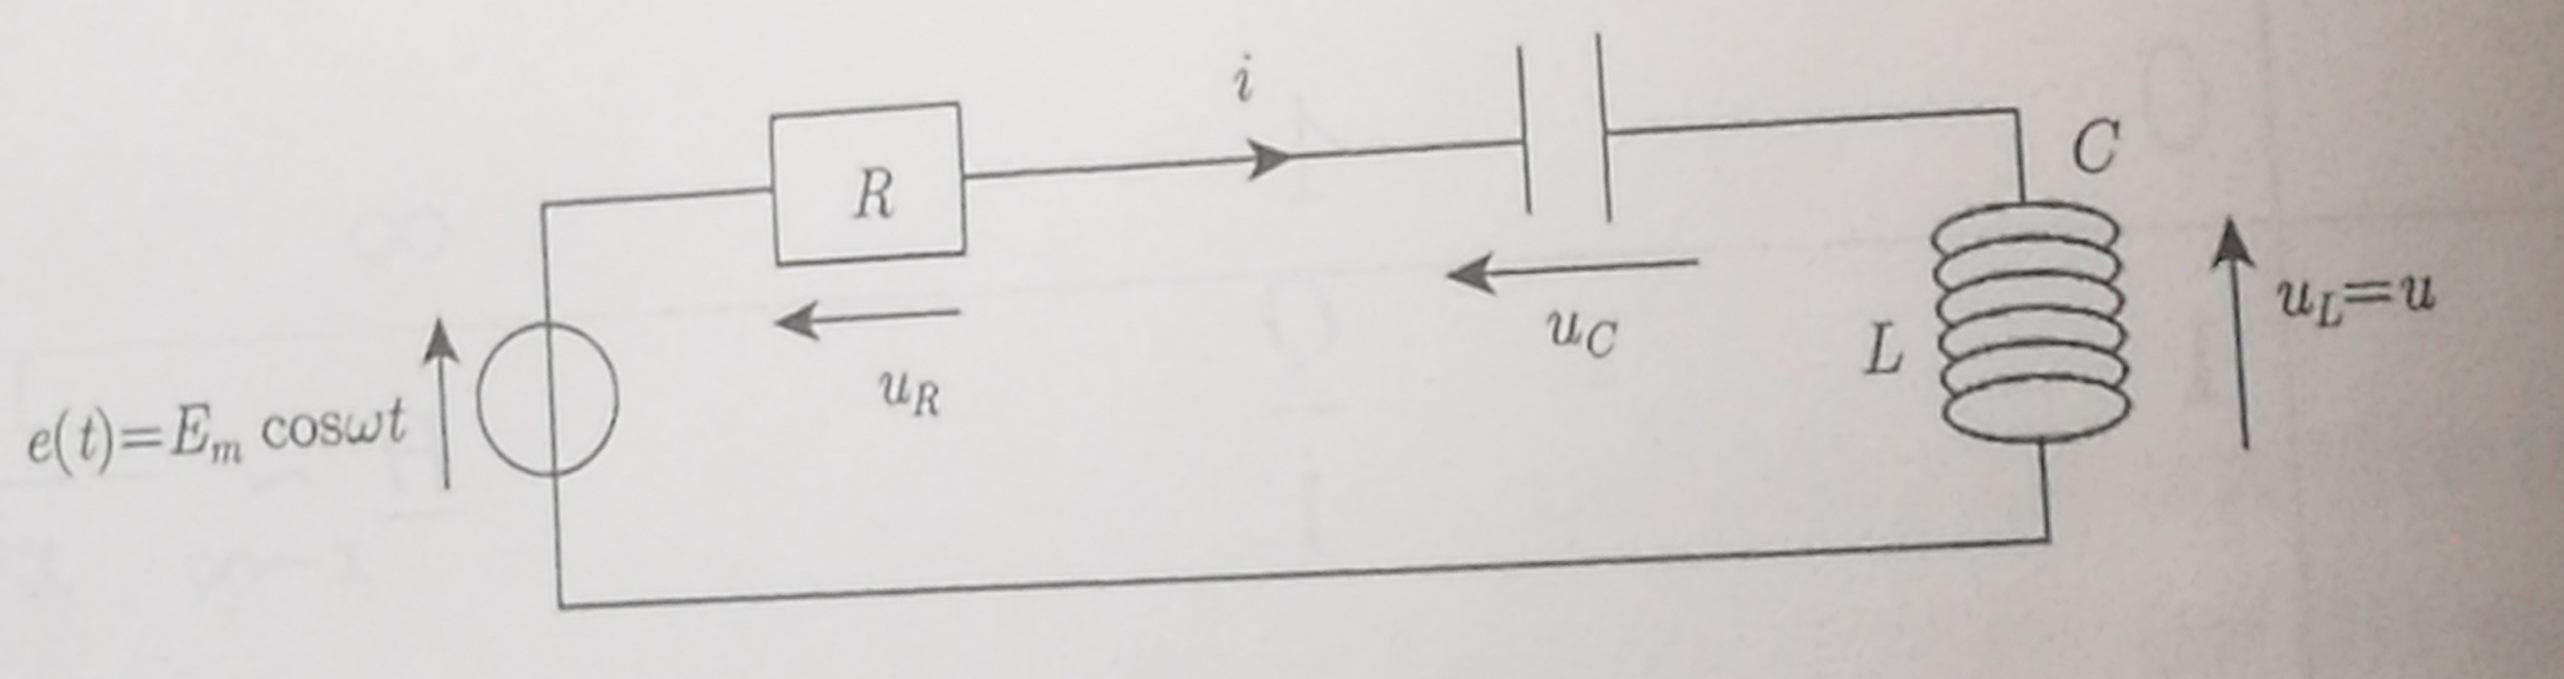
\includegraphics[scale=0.16]{Filtrage//5}
\end{figure}
\begin{itemize}
	\item \textbf{Comportement asymptotique}
	
	On a les ciruits équivalents suivants :
\begin{figure}[H]
	\centering
	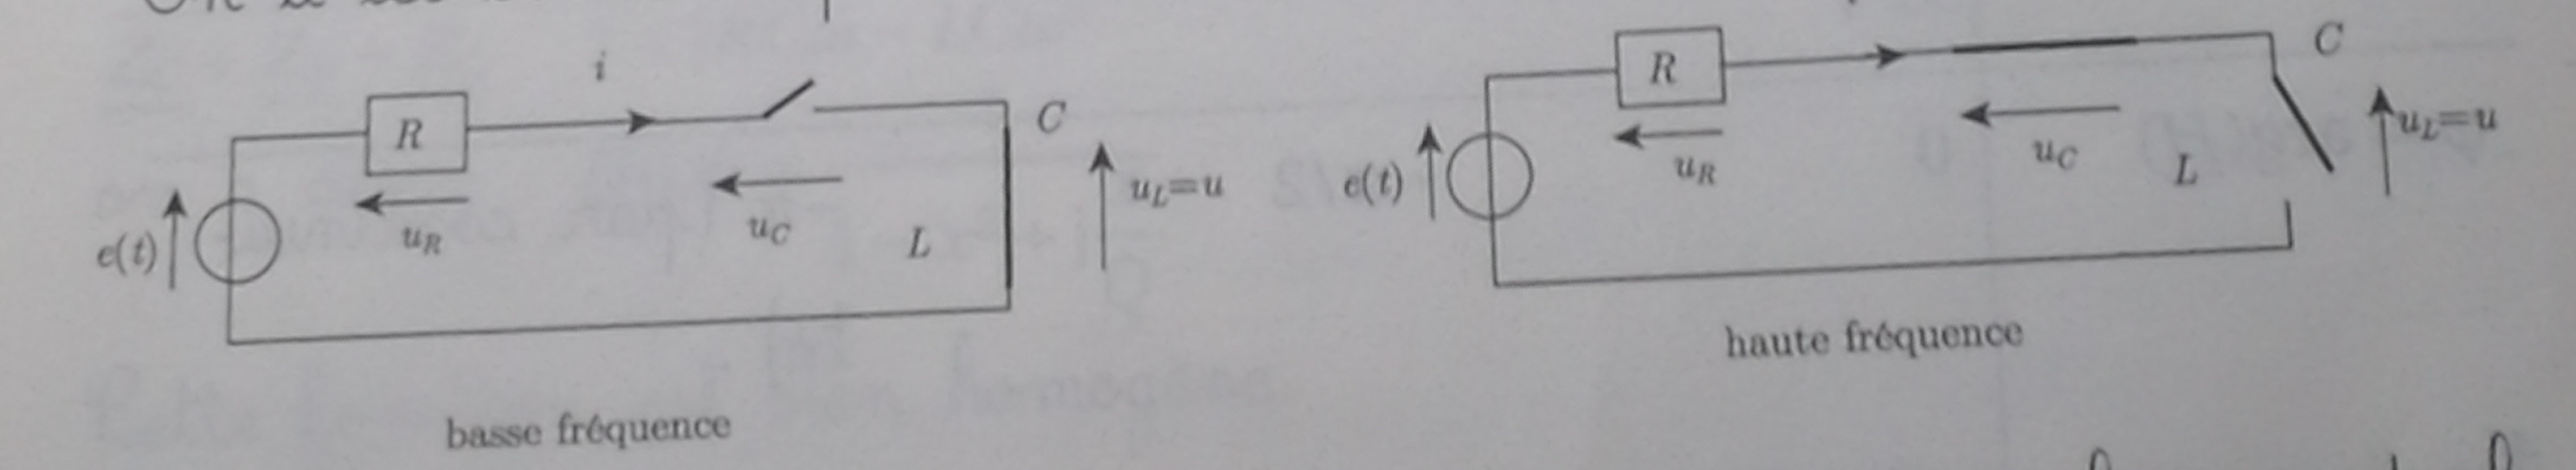
\includegraphics[scale=0.16]{Filtrage//6}
\end{figure}
低频时输出电压为0,高频时有输出电压,所以这是一个高通滤波器。

\item \textbf{Fonction de transfert}

$$
\underline{H}=\frac{\underline{Z}_L}{\underline{Z}_L+\underline{Z}_R+\underline{Z}_C}=\frac{jL\omega}{jL\omega+R+1/jC\omega}=\frac{1}{1+R/jL\omega+1/(-CL\omega^2)}=\frac{1}{1+1/jQx+1/(-x^2)}
$$
$$
\omega_0^2=1/CL
$$
$$
\frac{\omega_0}{Q}=R/L
$$
$$
\boxed{\underline{H}=\frac{-x^2}{1-x^2+j\frac{x}{Q}}}
$$

$$
G(x)=\frac{1}{\sqrt{(1-\frac{1}{x^2})^2+\frac{1}{Q^2x^2}}}
$$

$$
\phi(x)=-\arctan(\frac{x}{Q(1-x^2)})\quad \text{si}\quad x>1
$$
$$
\phi(x)=\pi-\arctan(\frac{x}{Q(1-x^2)})\quad \text{sinon}
$$
注意这里的$\pi$ 是根据$x\to0$时的Fresnel图得出相位差为$+\pi$,进而确定的。

然后我们开始研究Bode图。首先写出$G_{dB}=-10\log((1-\frac{1}{x^2})^2+\frac{1}{Q^2x^2})$
然后研究极限情况:
$$
\lim\limits_{x\to0}\phi(x)=\pi
$$
$$
\lim\limits_{x\to\infty}\phi(x)=0
$$
$$
\lim\limits_{x\to\infty}G_{dB}=0
$$
$$
G_{dB}\underset{x\to0}{\sim}40\log(x)
$$
另外,$x=1$处的情况也很重要,因为一方面这是谐振($x_r=\frac{1}{1-\frac{1}{2Q^2}}$)的附近值,可以反映是否出现超过电源电压振幅的电压,如果出现谐振还可以用于估计谐振峰值,另一方面这点是$\phi(x)$表达式的分段点,所以有重要的价值。
$$
G_{dB}(1)=20\log Q
$$
$$
\phi(1)=\pi/2
$$
\end{itemize}

\begin{figure}[H]
	\centering
	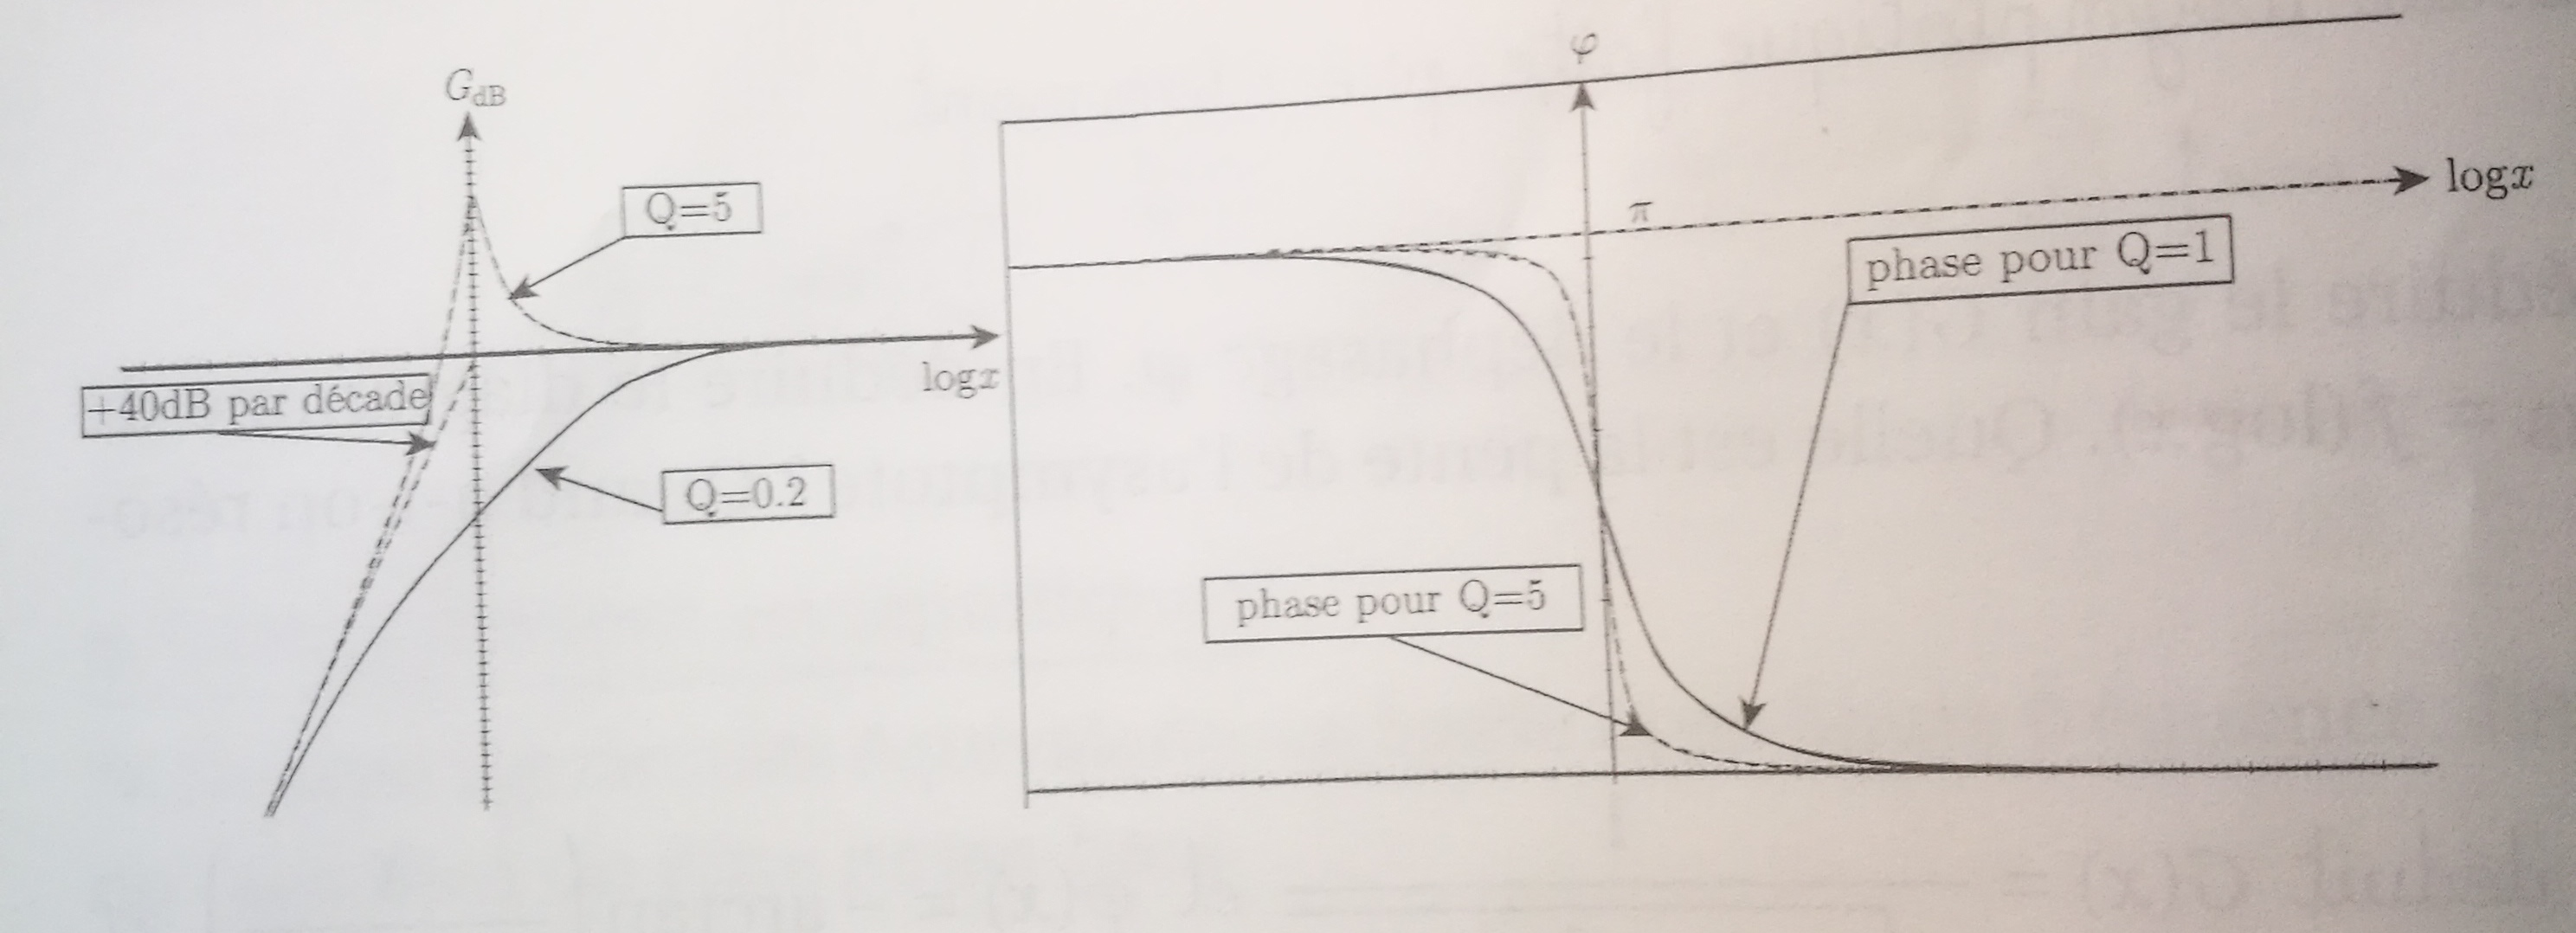
\includegraphics[scale=0.15]{Filtrage//7}
\end{figure}

\subsection{Filtre coupe-bande}
\begin{framed}{\textbf{框架}}
	On s'intéresse dans le circuit suivant à la réponse en tension aux bornes de la résistance.
\end{framed}
\begin{figure}[H]
	\centering
	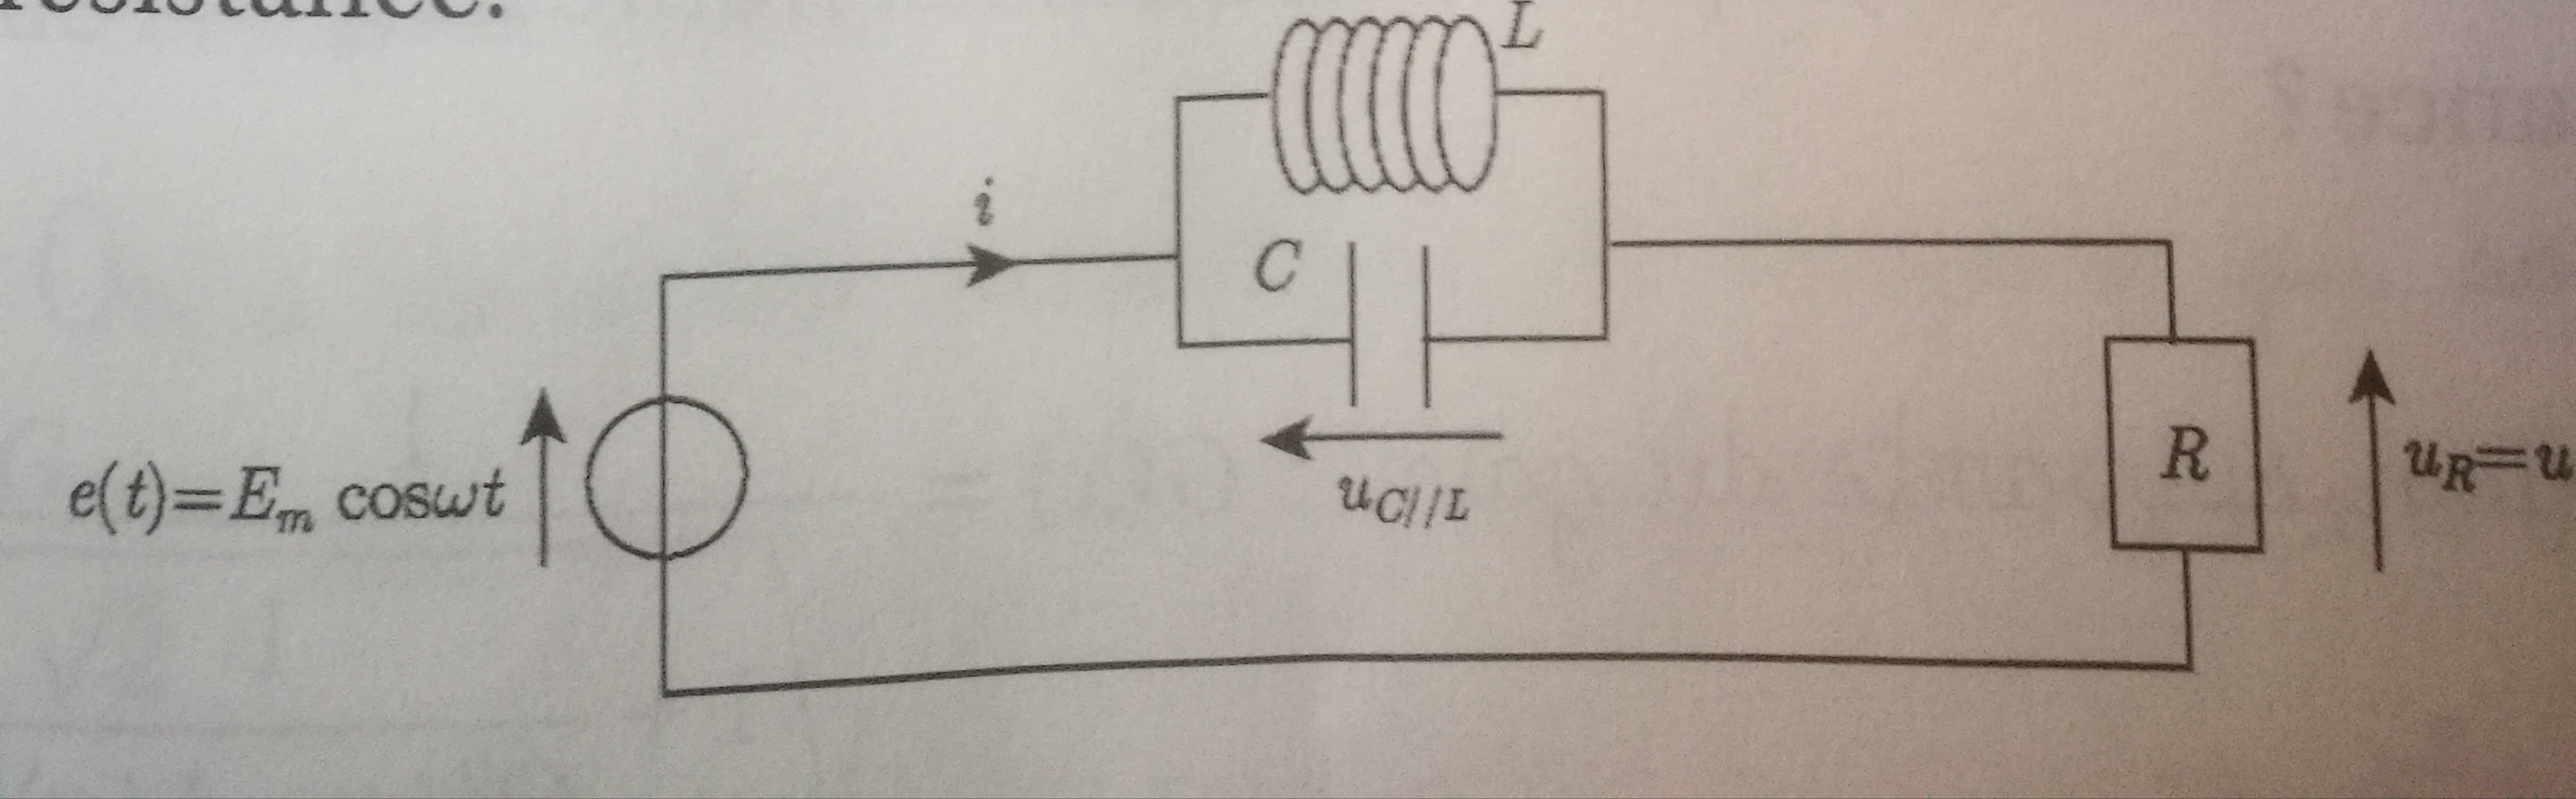
\includegraphics[scale=0.16]{Filtrage//8}
\end{figure}
\begin{itemize}
	\item \textbf{Comportement asymptotique}
	
	On a les ciruits équivalents suivants :
	\begin{figure}[H]
		\centering
		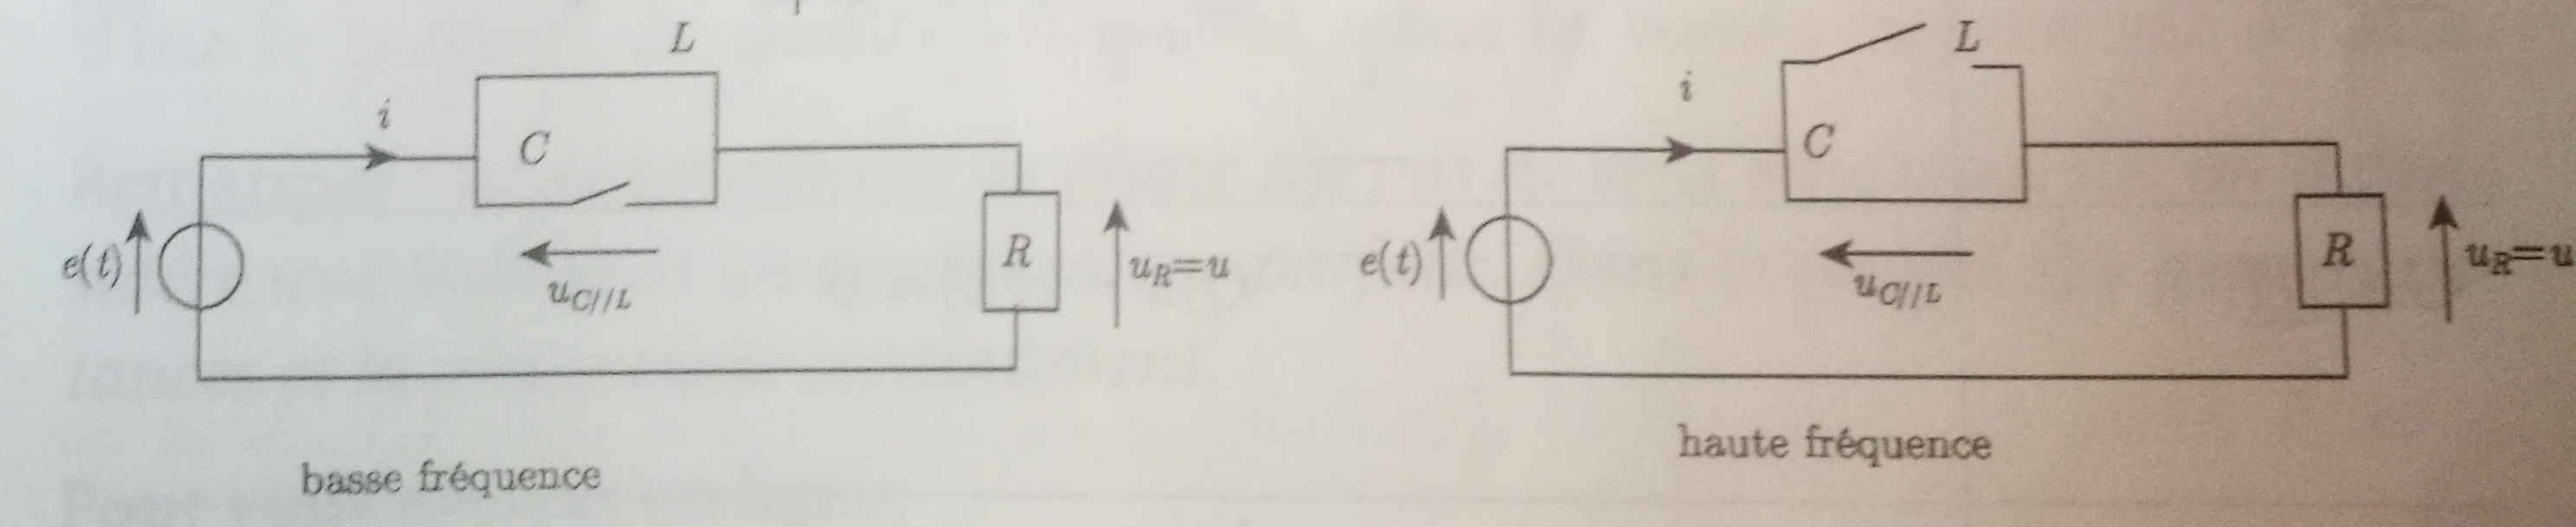
\includegraphics[scale=0.16]{Filtrage//9}
	\end{figure}
此时无论高频低频都有信号传出,只是中间可能有部分被阻断,所以叫“带阻”。



\item \textbf{Fonction de transfert}
$$
\underline{H}=\frac{\underline{Z}_R}{\underline{Z}_R+\underline{Z}_{||}}=\frac{R}{R+\frac{1}{\frac{1}{j\omega L}+j\omega C}}=\frac{1}{1+\frac{1}{\frac{R}{j\omega L}+j\omega CR}}=\frac{1}{1+\frac{1}{j(-\frac{R}{\omega L}+\omega CR)}}
$$
为了得到对应的$\omega_0$和$Q$,我们从传递函数逆列出微分方程:
$$
\frac{\underline{v}_s}{\underline{v}_e}=\frac{jR(-\frac{1}{\omega L}+\omega C)}{jR(-\frac{1}{\omega L}+\omega C)+1}=\frac{R(1-\omega^2 CL)}{R(1-\omega^2 CL)+j\omega L}
$$
$$
\underline{v}_sR-\underline{v}_s\omega^2 RCL+\underline{v}_sj\omega L=\underline{v}_eR-\underline{v}_e\omega^2 RCL
$$
$$
R\underline{v}_s+RCL\frac{\mathrm{d^2}\underline{v}_s}{\mathrm{d}t^2}+L\frac{\mathrm{d}\underline{v}_s}{\mathrm{d}t}=R\underline{v}_e+RCL\frac{\mathrm{d^2}\underline{v}_e}{\mathrm{d}t^2}
$$
$$
1/CL\underline{v}_s+\frac{\mathrm{d^2}\underline{v}_s}{\mathrm{d}t^2}+1/RC\frac{\mathrm{d}\underline{v}_s}{\mathrm{d}t}=1/CL\underline{v}_e+\frac{\mathrm{d^2}\underline{v}_e}{\mathrm{d}t^2}
$$
$$\omega_0^2=1/CL$$
$$\omega_0/Q=1/RC$$
$$\boxed{  \underline{H}=\frac{1}{1+\frac{1}{jQ(x-1/x)}}}  $$
$$
G(x)=\frac{1}{\sqrt{1+\frac{1}{Q^2(x-1/x)^2}}}
$$
$$
G_{dB}(x)=-10\log(1+\frac{1}{Q^2(x-1/x)^2})
$$
$$
\phi(x)=-\arctan(1/(Q(x-1/x)))
$$
$$
\lim\limits_{x\to0}\phi(x)=0
$$
$$
\lim\limits_{x\to\infty}\phi(x)=0
$$
$$
\lim\limits_{x\to0}G_{dB}(x)=0
$$
$$
\lim\limits_{x\to\infty}G_{dB}(x)=0
$$
$$
\lim\limits_{x\to1^{-}}\phi(x)=\pi/2
$$
$$
\lim\limits_{x\to1^{+}}\phi(x)=-\pi/2
$$
$$
\lim\limits_{x\to1^{-}}G_{dB}(x)=-\infty
$$
$$
\lim\limits_{x\to1^{+}}G_{dB}(x)=-\infty
$$
从而$G_{dB}(logx)$在$\log(1)=0$处有一条竖直渐近线(anti-résonance).
\end{itemize}
\begin{figure}[H]
	\centering
	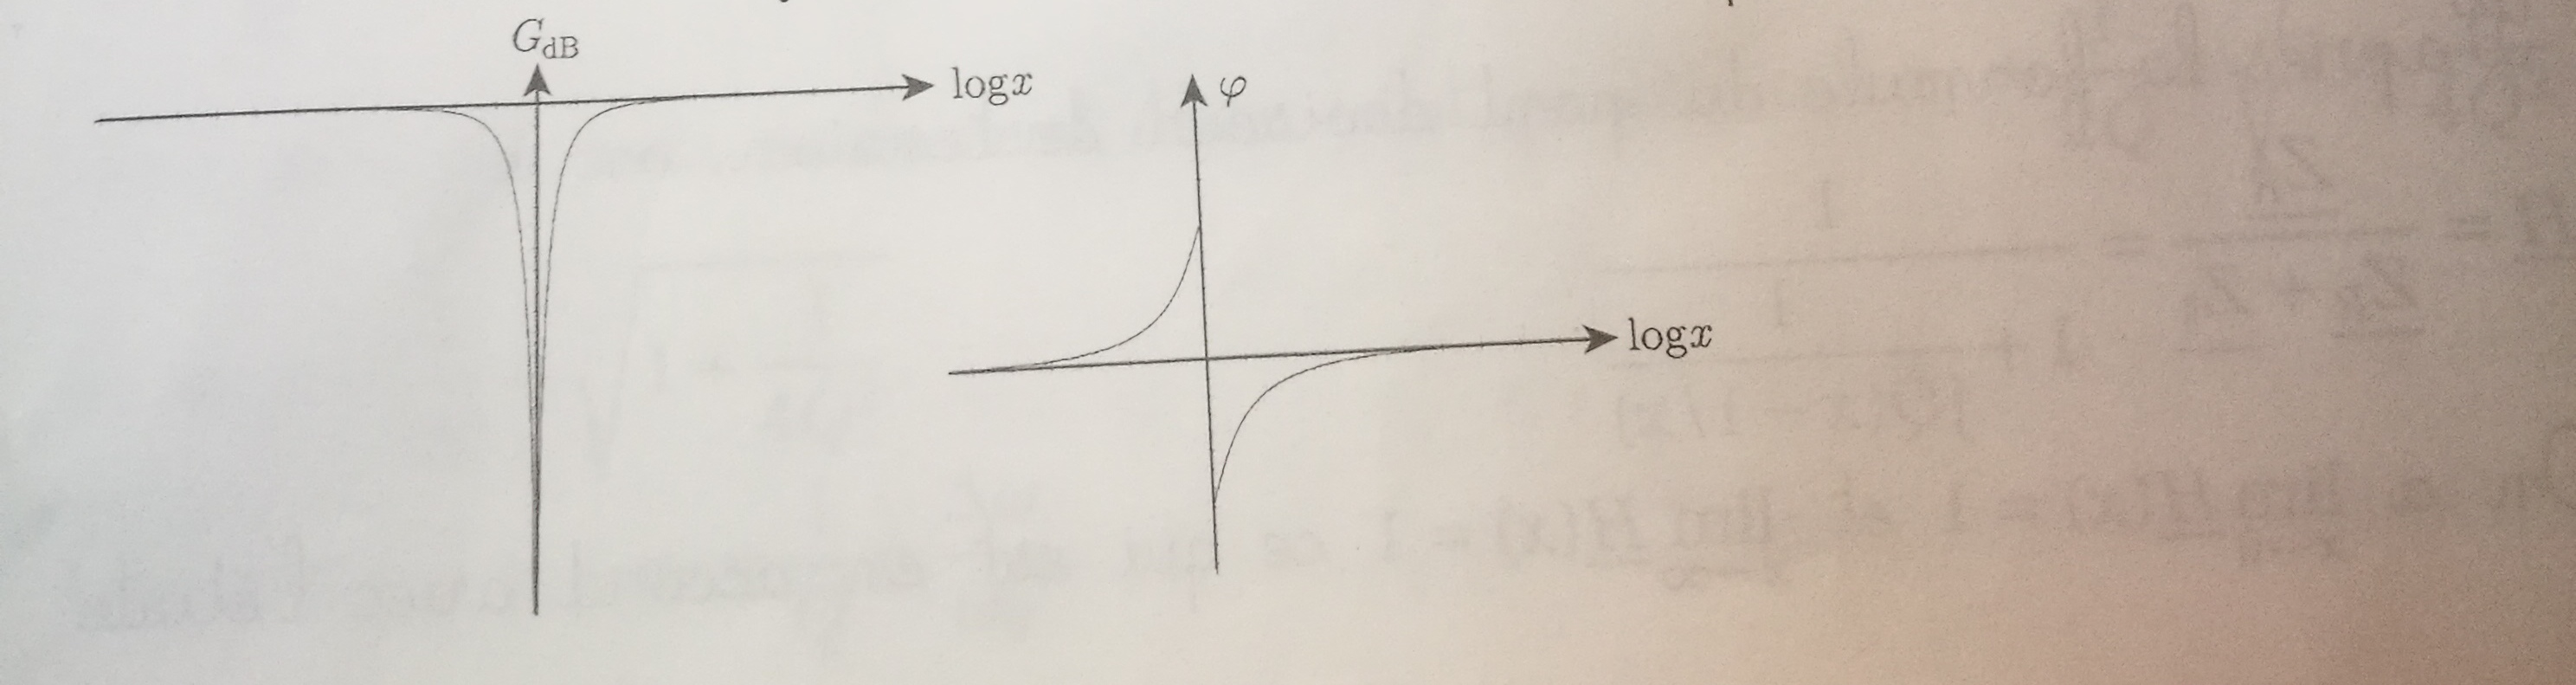
\includegraphics[scale=0.15]{Filtrage//10}
\end{figure}

\begin{framed}
	在带阻滤波器中,我们不定义通带,而定义阻带(la bande rejetée) $G_{dB}(\omega)\le G_{dB,max}-3dB$.
	
	阻带长度为$1/Q$,所以$Q$越大,阻带越窄。
\end{framed}	
\begin{framed}{\textbf{Critère de stabilité}}
	
	Un système est dit stable si la grandeur de sortie ne diverge pas.	
	
	Stabilité du filtre = Coefficients de l'équation différentielle homogène(由传递函数联系的$\underline{v_e}$和$\underline{v_s}$的关系式转化成的微分方程) de {\color{red}même signe}.
	
\end{framed}

\subsection{Filtres d'ordre plus élevé}
\begin{framed}{\textbf{定理}}
On n'étudie pas d'autres filtres car d'après le cours de mathématiques sur les polynômes(théorème d'Alembert-Guass),tout polynôme en $x$ est factorisable en polynômes de degré 1 ou 2. On peut donc étudier n'importe quelle fonction de transfert qui est décomposable en filtres du premier et du second ordre ,Ainsi l'étude d'un filtre d'ordre élevé se ramène à l'étude de filtres d'ordre un et deux.
$$
\underline{H}_{total}=\prod_{k=1}^{n}\underline{H}_k(\omega)
$$ 
\end{framed}
\section{Mise en cascade de filtres}
\subsection{Impédances d'entrée et de sortie}
On a vu qu'un quadripôle est caractérisé par 4 grandeurs : $e,u_s,i_e,i_s$.

On définit l'impédance d'entrée d'un dipôle comme:
$\underline{Z}_e=\frac{\underline{e}}{\underline{i}_e}$.Ainsi, vue de l'entrée ,un quadripôle est comme une source de tension $\underline{e}$ connectée à un dipôle en série d'impedance $\underline{Z}_e$

La sortie d'un quadripôle se comporte pour la charge(le reste du circuit) comme un dipôle actif dont l'impédance du générateur de Thévenin équivalent est appelée impudence de sortie $\underline{Z}_s$.Elle ne dépende que de la constitution du dipôle(指从输出端的角度看,四级子是一个可等效为戴维南电源的二端元件).
\begin{figure}[H]
	\centering
	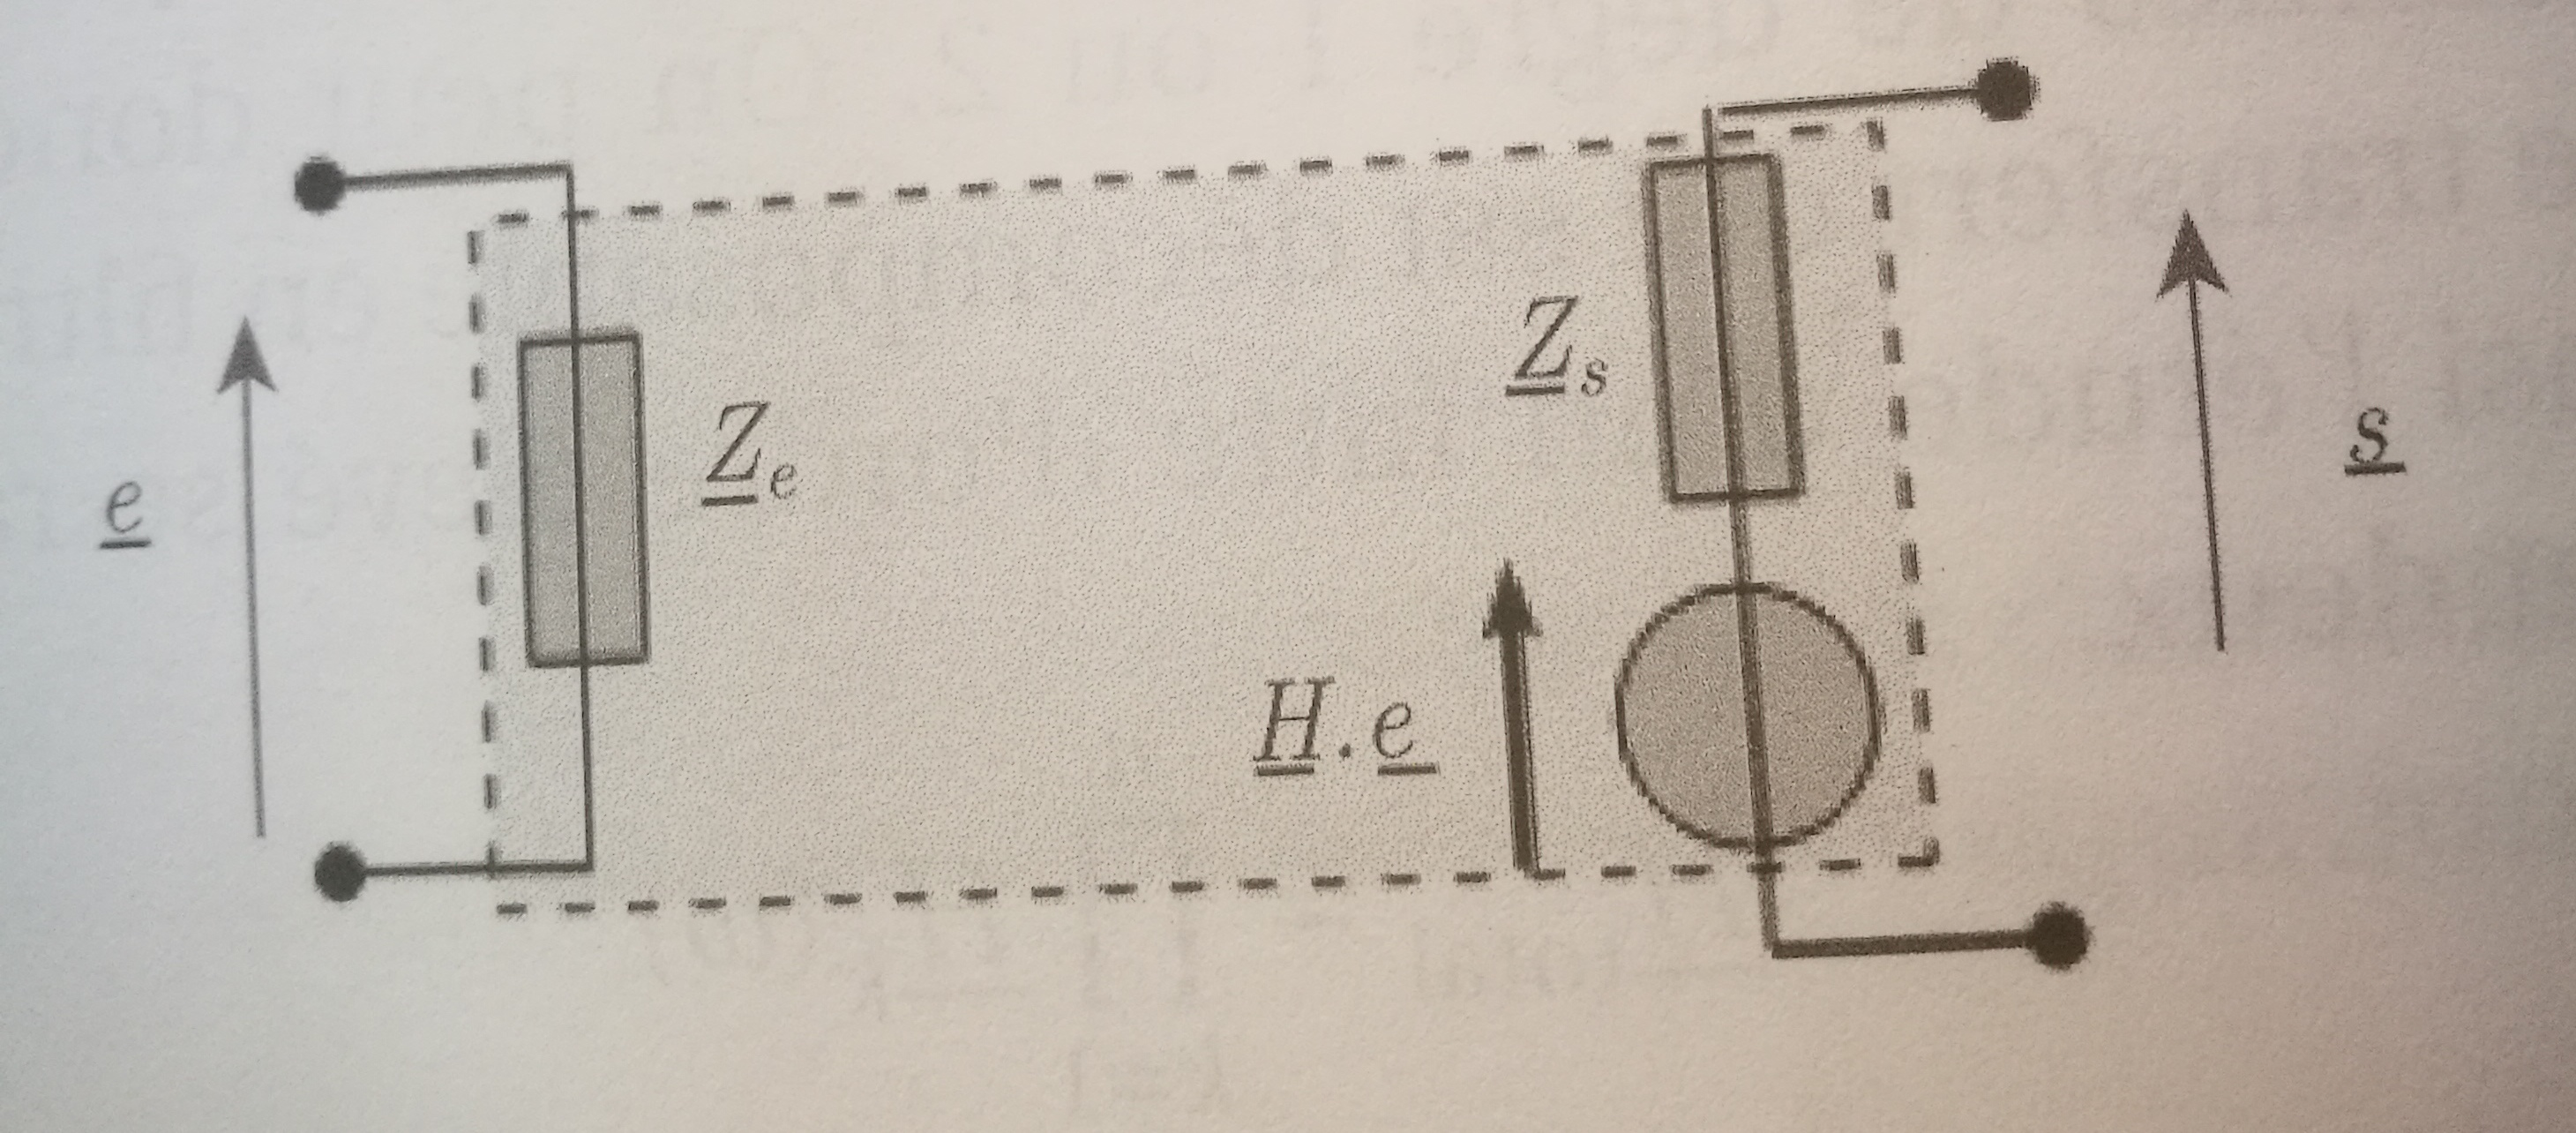
\includegraphics[scale=0.15]{Filtrage//11}
\end{figure}
\subsection{Mise en cascade}
\begin{framed}{\textbf{框架}}
 On s'intéresse à un montage avec un courant de sortie non nul.
\end{framed}
\begin{figure}[H]
	\centering
	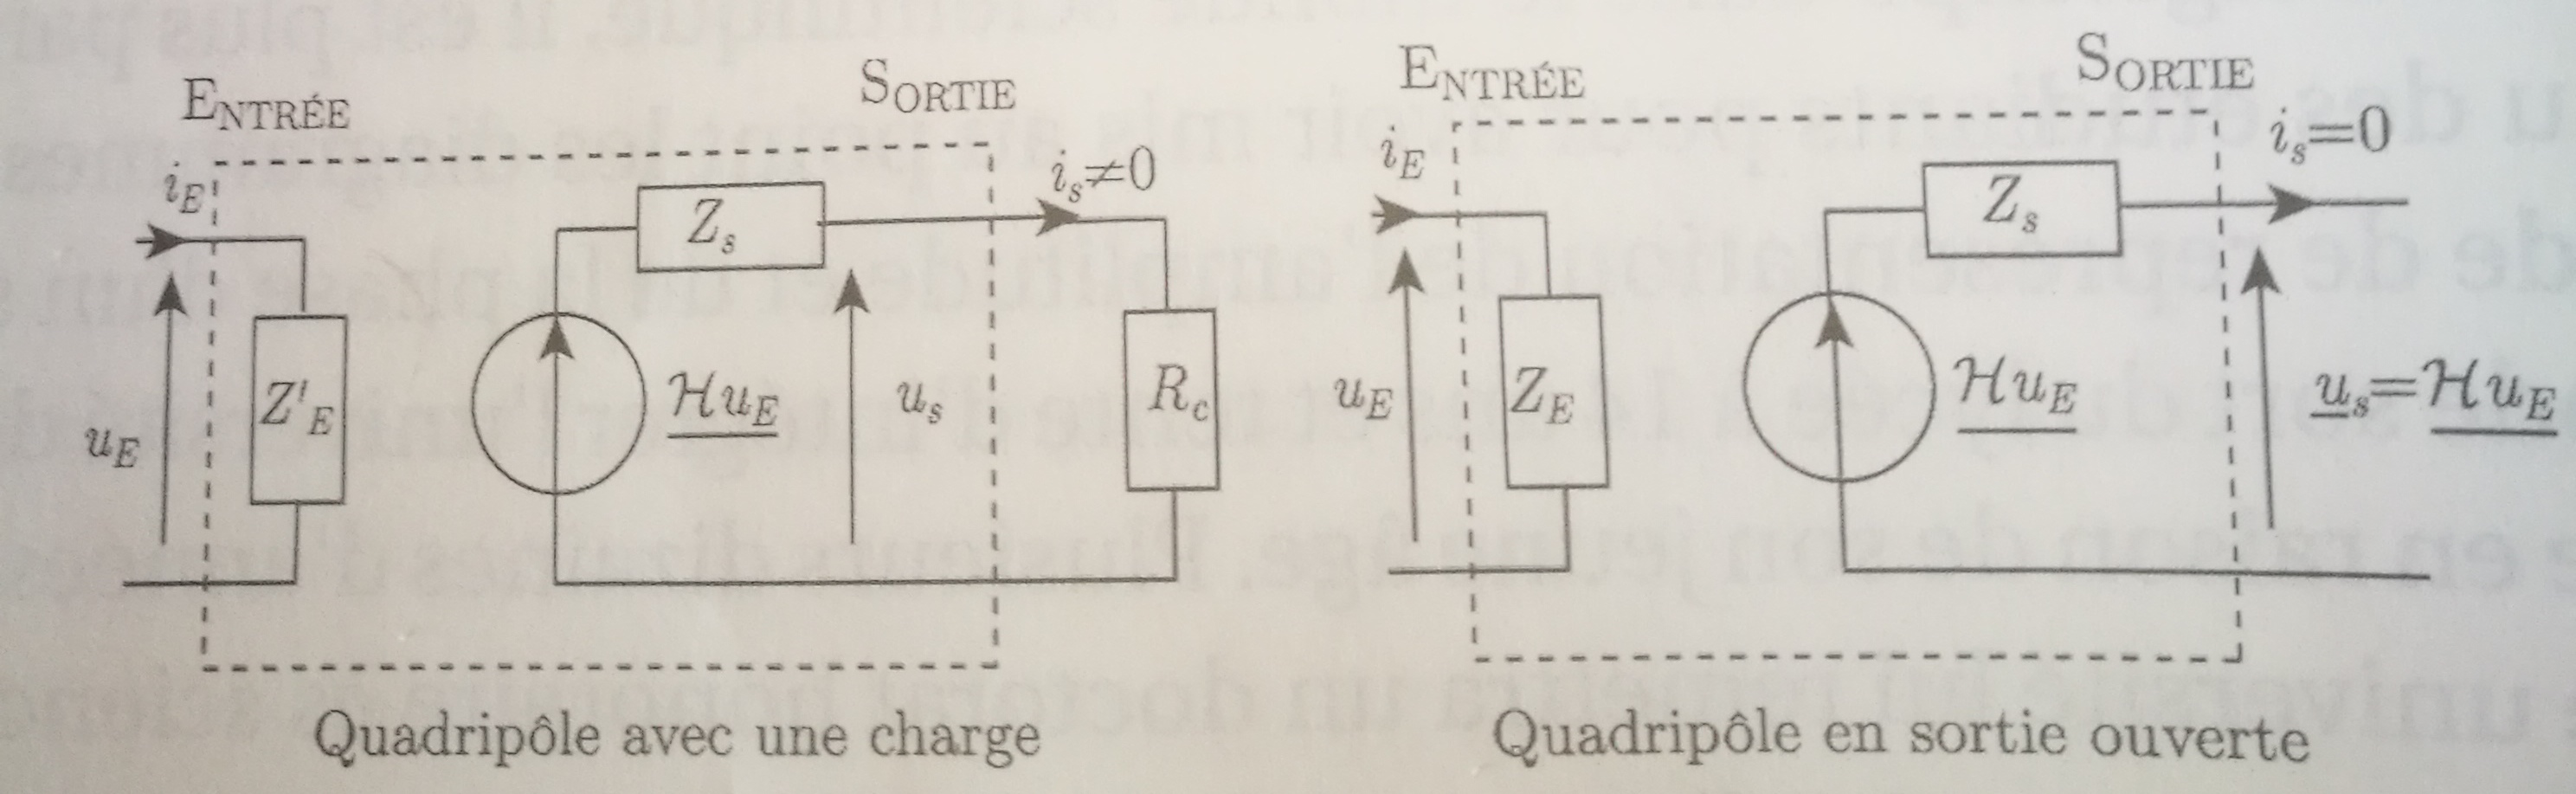
\includegraphics[scale=0.15]{Filtrage//12}
\end{figure}
On appelle $G_1$ et $G_2$ les gains en tension à vide des 2 filtres.
\begin{framed}
À quelle condition a-t-on $\frac{\underline{v}_{s2}}{\underline{e}_g}=\underline{G}_1\cdot\underline{G}_2$ {\color{red}quelles que noient} les vapeurs de l'impédance de charge(ou utile )$\underline{Z}_u$ et de l'impédance du générateur $\underline{Z}_g$?
\end{framed}




On a, par diviseur de tension:
\begin{framed}
$$
\begin{aligned}
\frac{\underline{v}_{s2}}{\underline{e}_g}&=\frac{\underline{v}_{s2}}{\underline{v}_{e2}}\cdot\frac{\underline{v}_{e2}}{\underline{v}_{e1}}\cdot\frac{\underline{v}_{e1}}{\underline{e}_g}\\
&=\underbrace{\frac{\underline{Z}_u}{\underline{Z}_u+\underline{Z}_{s2}}}_{A}\underline{G}_2\cdot\underbrace{\frac{\underline{Z}_{e2}}{\underline{Z}_{e2}+\underline{Z}_{s1}}}_{B}\underline{G}_1\cdot\underbrace{\frac{\underline{Z}_{e1}}{\underline{Z}_g+\underline{Z}_{e1}}}_{C}\\
&=\underline{G}_2\cdot\underline{G}_1
\end{aligned}
$$
\end{framed}
Cette dernière égalité implique que $A$,$B$ et $C$ valent chacun 1.On a donc 
\begin{framed}
\begin{itemize}
	\item $A=1$: $\forall \underline{Z}_u,  \underline{Z}_{s2}\ll \underline{Z}_u$ ce qui est réalisé pour $\underline{Z}_{s2}=0$
	\item $B=1$: $\forall \omega, \underline{Z}_{s1}\ll \underline{Z}_{e2}$ ce qui est réalisé pour $\underline{Z}_{e2}=\infty$ ou $\underline{Z}_{s1}=0$
	\item $C=1$: $\forall \underline{Z}_g,  \underline{Z}_{g}\ll \underline{Z}_{e1}$ ce qui est réalisé pour $\underline{Z}_{e1}=\infty$
\end{itemize}
\end{framed}
若电源为理想电压源,且第二个filtre “en sortie ouverte”,则:$A=1$且$C=1$成立。那么要使两个filtre之间没有电流,则只要$B=1$的条件成立即可。











\chapter{Classical Mechanics}
\section{The Moving Trihedral(Accompanying Dreibein)-the Frenet Formulas}

In some cases it may be simpler to express velocity and acceleration in $\mathit{natural}$ $\mathit{coordinates}$.
This means that the velocity and acceleration are not derived from the variation of the position vector with time ,but from its variation with its the  passed way $s$, the arc length, the starting point being arbritrary 

In order to become independent of the coordinate frame, a set of orthogonal unit vectors
is put at the point of the trajectory of the mass point given by $s$.
The set of unit vectors moves along with the mass point : it is therefore also called the "moving trihedral" or "accompanying dreibein"
\paragraph{Darbaux rotation vecteur}
The Fernet's formulas can be formulated in a very elegant way.To this end, we define a vector $\mathbf{D}$ as follows:
$$\mathbf{D}=\tau \mathbf{T}+\kappa \mathbf{B}$$
\end{document}